\documentclass[11pt,a4paper,titlepage,openright,oneside]{book}

\usepackage{ft2unb}

\usepackage{graphicx}
\usepackage{amsfonts}
\usepackage{amsmath}
\usepackage{amssymb}
\usepackage[thmmarks,amsmath]{ntheorem}
\usepackage{boxedminipage}
\usepackage{theorem}
\usepackage{fancybox}
\usepackage{fancyhdr}
\usepackage{url}
\usepackage{afterpage}
\usepackage{color}
\usepackage{colortbl}
\usepackage{rotating}
\usepackage{makeidx}
\usepackage{indentfirst}
\usepackage{bibentry}
\usepackage{subcaption}
\usepackage{listings}
\usepackage[obeyDraft]{todonotes}
\presetkeys{todonotes}{inline}{}
\def\compilewholereport{}
\newcommand\qt[1]{\lq\lq{}#1\rq\rq{}}
\newcommand\qti[1]{\lq\lq{}\textit{#1}\rq\rq{}}

\makeindex
 
%%%%%%%%%%%%%%%%%%%%%%%%%%%%%%%%%%%%%%%%%%%%%%%%%%%%%%%%%%%%%%%%%%%%%%%%%
% Compilações parciais: com o comando abaixo, selecione apenas os capitulos
% que deseja compilar. Por exemplo, veja o que acontece se descomentar a 
% linha abaixo:
%\includeonly{resumos}
%%%%%%%%%%%%%%%%%%%%%%%%%%%%%%%%%%%%%%%%%%%%%%%%%%%%%%%%%%%%%%%%%%%%%%%%%

%%%%%%%%%%%%%%%%%%%%%%%%%%%%%%%%%%%%%%%%%%%%%%%%%%%%%%%%%%%%%%%%%%%%%%%%%
% Documento principal
%%%%%%%%%%%%%%%%%%%%%%%%%%%%%%%%%%%%%%%%%%%%%%%%%%%%%%%%%%%%%%%%%%%%%%%%%
\begin{document}

\grau{Engenheiro de Controle e Automa\c{c}\~ao} \tipodemonografia{Trabalho de Gradua\c{c}\~ao}

% Os comandos a seguir servem para definir o título do trabalho. Para evitar 
% que o latex defina automaticamente a quebra de linha, foram definidos um comando por linha. 
% Desta forma o autor define como quer que o título seja dividio em várias linhas. 
% O exemplo abaixo é para um título que ocupa três linhas. Observe que mesmo com a linha
% 4 não sendo utilizada, o comando \titulolinhaiv é chamado.
\titulo{Estudo e Implementa\c{c}\~ao de Reconfigura\c{c}\~ao \mbox{Din\^amica} Em Instrumenta\c{c}\~ao, Automa\c{c}\~ao e Controle}

% Os nomes dos autores são definidos pelos comandos \autori (autor 1) e \autorii (autor 2).
% Para trabalhos com apenas um autor, deve-se usar \autorii{} para que não apareça 
% um nome para segundo autor.
\autor{Lucas Sousa de Oliveira}
 
% Os nomes dos membros da banca são definidos a seguir. Pode-se ter até 5 membros da banca.
% É incubência do usuário definir no argumento dos comandos a afiliação do membro da banca,
% assim como sua posição (se for orientador ou co-orientador). 
% Os nomes definidos pelos comandos abaixo aparecem na ordem de i a v.
\membrodabanca{Prof. Jones Yudi}{ENM/UnB}{Orientador}
\membrodabanca{Prof. Carlos Humberto Llanos}{ENM/UnB}{Co-orientador}
\membrodabanca{Prof. Daniel Muñoz Arboleda}{FGA/UnB}{Examinador externo}
\membrodabanca{M.Sc. Janier Arias Garcia}{ENM/UnB}{Examinador interno}

% data de defesa: mês e ano.
%\mes{dezembro}
%\ano{2013}

% Comandos para criar a capa e a página de assinaturas.
\capaprincipal
\listoftodos
\capaassinaturas

%%%%%%%%%%%%%%%%%%%%%%%%%%%%%%%%%%%%%%%%%%%%%%%%%%%%%%%%%%%%%%%%%%%%%%%%%
% Dedicatória 
%%%%%%%%%%%%%%%%%%%%%%%%%%%%%%%%%%%%%%%%%%%%%%%%%%%%%%%%%%%%%%%%%%%%%%%%%
\frontmatter

% Texto de dedicatória do primeiro autor
\dedicatoria{Dedico este trabalho a meus pais Marconi e Marta Oliveira, a minha família, a minha namorada Ananda Medeiros, a todos os meus amigos, em especial a Emerson Grzeidak e a Kevin Gularte, e a todos os meus professores.}
%% Texto de dedicatória do segundo autor. Caso não tenha um segundo autor, este texto não será mostrado
%\dedicatoria{Dedicatória do autor 2}
%% Texto de dedicatória do terceiro autor. Caso não tenha um segundo autor, este texto não será mostrado
%\dedicatoria{Dedicatória do autor 3} 

% Comando para criar a página de dedicatória
\paginadededicatorias

%%%%%%%%%%%%%%%%%%%%%%%%%%%%%%%%%%%%%%%%%%%%%%%%%%%%%%%%%%%%%%%%%%%%%%%%%
% Agradecimentos
%%%%%%%%%%%%%%%%%%%%%%%%%%%%%%%%%%%%%%%%%%%%%%%%%%%%%%%%%%%%%%%%%%%%%%%%%
%\agradecimentos{A inclusão desta seção de agradecimentos é opcional e fica à critério do(s) autor(es), que caso deseje(em) inclui-la deverá(ao) utilizar este espaço, seguindo está formatação.}
%\agradecimentos{A inclusão desta seção de agradecimentos é opcional e fica à critério do(s) autor(es), que caso deseje(em) inclui-la deverá(ao) utilizar este espaço, seguindo está formatação.}
%\agradecimentosi{A inclusão desta seção de agradecimentos é opcional e fica à critério do(s) autor(es), que caso deseje(em) inclui-la deverá(ao) utilizar este espaço, seguindo está formatação.}

% Comando para criar a página de agradecimentos
%\paginadeagradecimentos

%%%%%%%%%%%%%%%%%%%%%%%%%%%%%%%%%%%%%%%%%%%%%%%%%%%%%%%%%%%%%%%%%%%%%%%%%
% Resumo: arquivo resumo.tex editável no Scientific Word
%%%%%%%%%%%%%%%%%%%%%%%%%%%%%%%%%%%%%%%%%%%%%%%%%%%%%%%%%%%%%%%%%%%%%%%%%
%TCIDATA{LaTeXparent=0,0,relatorio.tex}

\resumo{Resumo}{
A reconfiguração dinâmica de circuitos digitais representa o estado da arte em tecnologias de computação reconfigurável.
Através dela é possível reduzir o gasto energético, simplificar projetos, aumentar o desempenho geral do projeto e até resolver problemas antes impossíveis.
Este estudo buscou conhecer e apresentar as ferramentas e tecnologias necessárias para o desenvolvimento de um projeto deste tipo. Os cinco experimentos realizados também serviram para demonstrar e explicar o uso de alguns periféricos úteis, tais como memórias Flash e RAM, o HWICAP (necessário para a reconfiguração), a interface UART, dentre outros.
Neles, também foram descritos os processos necessários para o desenvolvimento de periféricos customizados, podendo, inclusive, serem reconfiguráveis.
Os resultados obtidos em cada experimento apresentam considerações importantes na opção pelo uso dessa tecnologia.
Conseguiu-se, por fim, definir um fluxo de projeto genérico que pode ser utilizado em grande parte dos projetos que necessitam de reconfiguração dinâmica.}

\paragraph{Palavras Chave:} Reconfiguração Dinâmica; Autorreconfiguração; MicroBlaze; DDR3; Xilinx; Periféricos.

\vspace*{2cm}

\resumo{Abstract}{
The dynamic reconfiguration of digital circuitry represents the state-of-art in reconfigurable computation.
By using it it's possible to reduce the power, simplify projects, increase the overall system performance and even solve otherwise unsolvable problems.
This study tried to explore and present the tools and technologies required to develop a project that used dynamic reconfiguration.
The five experiments performed were also used to demonstrate and explain the use of a series of useful peripherals, such as Flash and RAM memories, the HWICAP peripheral, and the UART interface, and to describe the process required to build custom peripherals, including reconfigurable peripherals.
The results attained in each experiment are used to show important considerations when choosing this technology.
In the end, it was possible to define a generic project flow that can be used in most of the projects willing to use dynamic reconfiguration.}

\paragraph{Keywords:} Dynamic Reconfiguration; Self-reconfiguration; MicroBlaze; DDR3; Xilinx; Peripherals.

%%%%%%%%%%%%%%%%%%%%%%%%%%%%%%%%%%%%%%%%%%%%%%%%%%%%%%%%%%%%%%%%%%%%%%%%%
% Listas de conteúdo, figuras e tabelas.
%%%%%%%%%%%%%%%%%%%%%%%%%%%%%%%%%%%%%%%%%%%%%%%%%%%%%%%%%%%%%%%%%%%%%%%%%
\sumario
\listadefiguras
\listadetabelas

%%%%%%%%%%%%%%%%%%%%%%%%%%%%%%%%%%%%%%%%%%%%%%%%%%%%%%%%%%%%%%%%%%%%%%%%%
% Lista de simbolos.
%%%%%%%%%%%%%%%%%%%%%%%%%%%%%%%%%%%%%%%%%%%%%%%%%%%%%%%%%%%%%%%%%%%%%%%%%
%TCIDATA{LaTeXparent=0,0,these.tex}
                      

%\chapter*{\setfontarial\mdseries LISTA DE SÍMBOLOS} % se usar ft1unb.sty, descomente esta linha
\chapter*{LISTA DE SÍMBOLOS} % se usar ft2unb.sty, descomente esta linha

\subsection*{Siglas}

\begin{tabular}{p{0.1\textwidth}p{0.80\textwidth}}
FPGA & \textit{Field-Programmable Gate Array}\\
UART & \textit{Universal Assynchronous Receiver/Transmitter}\\
SPI & \textit{Serial Peripheral Interface}\\
\end{tabular}



%%%%%%%%%%%%%%%%%%%%%%%%%%%%%%%%%%%%%%%%%%%%%%%%%%%%%%%%%%%%%%%%%%%%%%%%%
% Corpo principal
%%%%%%%%%%%%%%%%%%%%%%%%%%%%%%%%%%%%%%%%%%%%%%%%%%%%%%%%%%%%%%%%%%%%%%%%%
\mainmatter
\setcounter{page}{1} \pagenumbering{arabic} \pagestyle{plain}

% *** Introducao ***
\part{Introdução}
%TCIDATA{LaTeXparent=0,0,relatorio.tex}
\ifx\compilewholereport\undefined
	\documentclass[11pt,a4paper,oneside]{book}
	
	% Escolher um dos seguintes formatos:
	\usepackage{ft2unb} % segue padrão de fontes do Latex
	
	% Pacotes
	\usepackage{graphicx}
	\usepackage{amsfonts}
	\usepackage{amsmath}
	\usepackage{amssymb}
	\usepackage[thmmarks,amsmath]{ntheorem}
	\usepackage{boxedminipage}
	\usepackage{theorem}
	\usepackage{fancybox}
	\usepackage{fancyhdr}
	\usepackage{url}
	\usepackage{afterpage}
	\usepackage{color}
	\usepackage{colortbl}
	\usepackage{rotating}
	\usepackage{makeidx}
	\usepackage{indentfirst}
	\usepackage{bibentry}
	\usepackage{subcaption}
	\usepackage{todonotes}
	\presetkeys{todonotes}{inline}{}
	
	\begin{document}
	\frontmatter
	\tableofcontents
	\mainmatter
	
	%%%%%%%%%%%%%%%%%%%%%%%%%%%%
	%%%%%%%% Apagar coisas acima
	%%%%%%%%%%%%%%%%%%%%%%%%%%%%
	\newcommand\qt[1]{\lq\lq{}#1\rq\rq{}}
	\newcommand\qti[1]{\lq\lq{}\textit{#1}\rq\rq{}}
\fi

\chapter{Introdu\c{c}\~ao}\label{CapIntro}

\resumodocapitulo{Este cap\'itulo contextualiza o tema do trabalho, apresentando a motivação histórica seu desenvolvimento, uma motivação tecnológica, seus objetivos e metodologia.}

\vspace{0.8cm}
O mundo atual \'e controlado quase que completamente por sistemas digitais.
As informa\c{c}\~oes obtidas pelos sensores s\~ao digitalizadas antes de serem tratadas.
Tal processo de digitaliza\c{c}\~ao \'e importante, visto que elimina os ru\'idos intr\'insecos ao processamento anal\'ogico \cite{chen2004electrical}.

O primeiro computador de computa\c{c}\~ao gen\'erica surgiu por volta da d\'ecada de 40.
Sua inven\c{c}\~ao iniciou a terceira revolu\c{c}\~ao industrial, conhecida como revolu\c{c}\~ao da informa\c{c}\~ao ou revolu\c{c}\~ao t\'ecnico-cient\'ifica-informacional \cite{patterson2005coa}.
Os computadores dessa \'epoca liam e executavam instru\c{c}\~oes de forma linear, em um modelo conhecido como sequencial ou temporal. 

Nos anos que se seguiram, a substituição das válvulas por transistores de sil\'icio ajudaram a reduzir o tamanho dos computadores de metros a cent\'imetros quadrados.
Tal mudan\c{c}a permitiu um aumento na popularidade destes dispositivos para o uso pessoal, efeito que impulsionou a ind\'ustria de produ\c{c}\~ao de processadores \cite{Hennessy2011}.
As empresas da \'epoca come\c{c}aram ent\~ao a guerra de miniaturiza\c{c}\~oes de transistores, marcada pelo c\'elebre artigo de Gordon E. Moore, cofundador da Intel, que dizia que o n\'umero de transistores dentro de um processador duplicaria aproximadamente a cada 2 anos \cite{Moore1965}.
A partir de 1970, a lei foi adaptada para a duplica\c{c}\~ao a cada 18 meses \cite{Hennessy2011}.
A figura \ref{fig:moores_law} apresenta uma visualização da lei de Moore nos anos que se seguiram.

\begin{figure}[h]
	\centering
	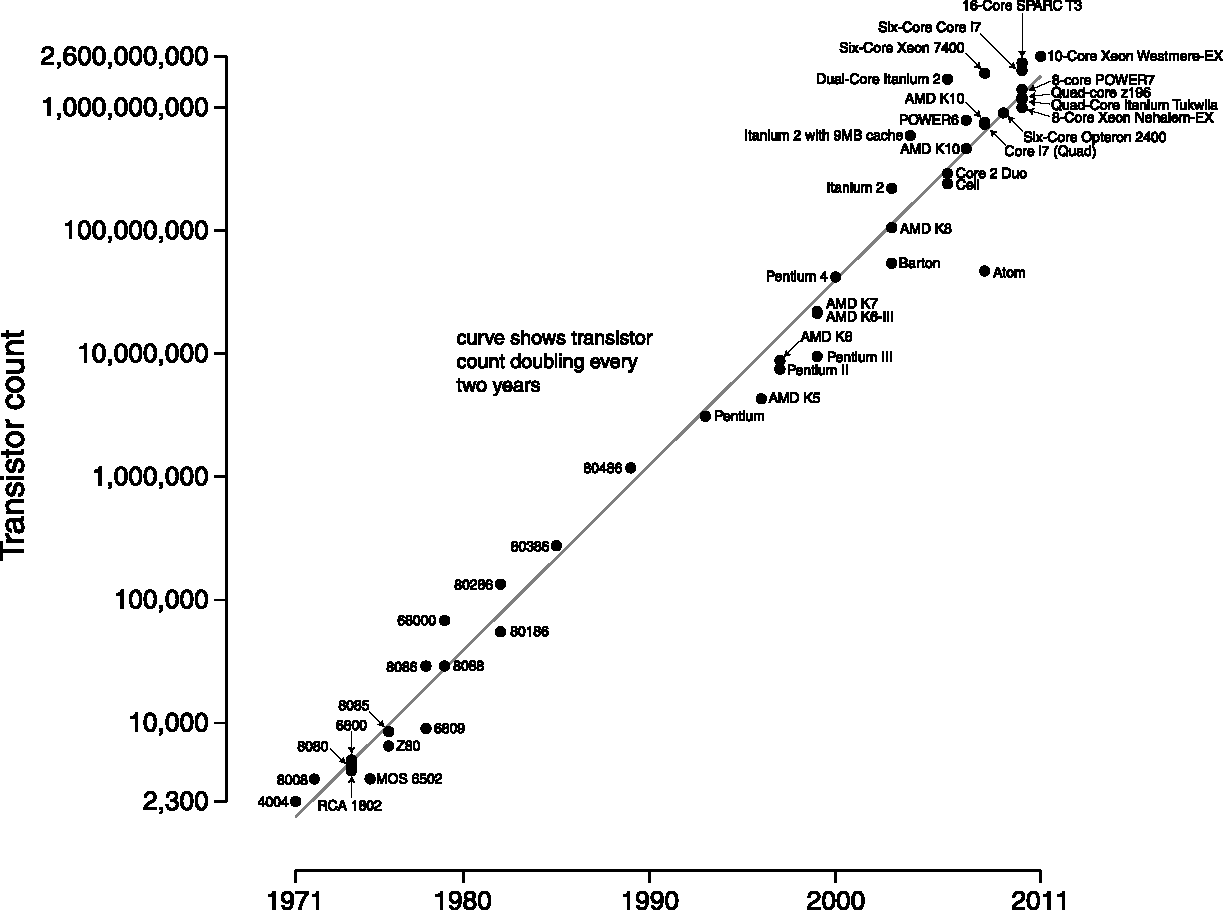
\includegraphics[width=0.7\textwidth]{fig/c1_introducao/moores_law.pdf}
	\caption{Visualização da Lei de Moore. Eixos em escala logarítmica. Extraido de \cite{moore2011}.}
	\label{fig:moores_law}
\end{figure}

Com a integra\c{c}\~ao de mais componentes dentro do processador, conjuntos de instru\c{c}\~oes cada vez mais complexas foram desenvolvidas.
Estas instru\c{c}\~oes surgiram para acelerar a computa\c{c}\~ao de fun\c{c}\~oes de n\'iveis mais altos.
A integra\c{c}\~ao tamb\'em reduziu a pot\^encia dissipada por transistor, permitindo que as frequ\^encias de opera\c{c}\~ao dos computadores fosse aumentada \cite{Hennessy2011}.

Com o aumento da complexidade das instruções, passou-se a adotar duas nomenclaturas diferentes para processadores: \textit{Reduced Instruction Set Computer} (RISC) e \textit{Complex Instruction Set Computer} (CISC) \cite{Fedeli2003}.
A arquitetura RISC possui um conjunto pequeno e muito otimizado de funções, comandos exclusivos para acesso a memória (arquitetura \textit{load/store}) e uma média de uma instrução completada por ciclo, quando desconsidera-se as instruções de acesso a memória.
A arquitetura CISC possui várias funções para tarefas mais específicas, que por vezes demandam vários ciclos de relógio, e funções que realizam operações com informações lendo e/ou salvando direto na/para a memória.
A arquitetura RISC, que possui em seu portfolio dispositivos como ARM, IBM PowerPC, Sun SPARK e MIPS, dentre outros, é muito mais utilizada nos dias de hoje.
A figura \ref{fig:history_risc} mostra um pouco da história desta arquitetura.
Até empresas como a Intel, que ficaram populares com seus processadores CISC, tem se curvado a arquitetura RISC devido a seu uso mais eficiente de potência.
Eles vem utilizando uma arquitetura conhecida como núcleo de RISC (\textit{RISC core}), onde as instruções são recebidas em formato CISC e decodificadas para uma arquitetura interna RISC.

\begin{figure}[h]
\centering
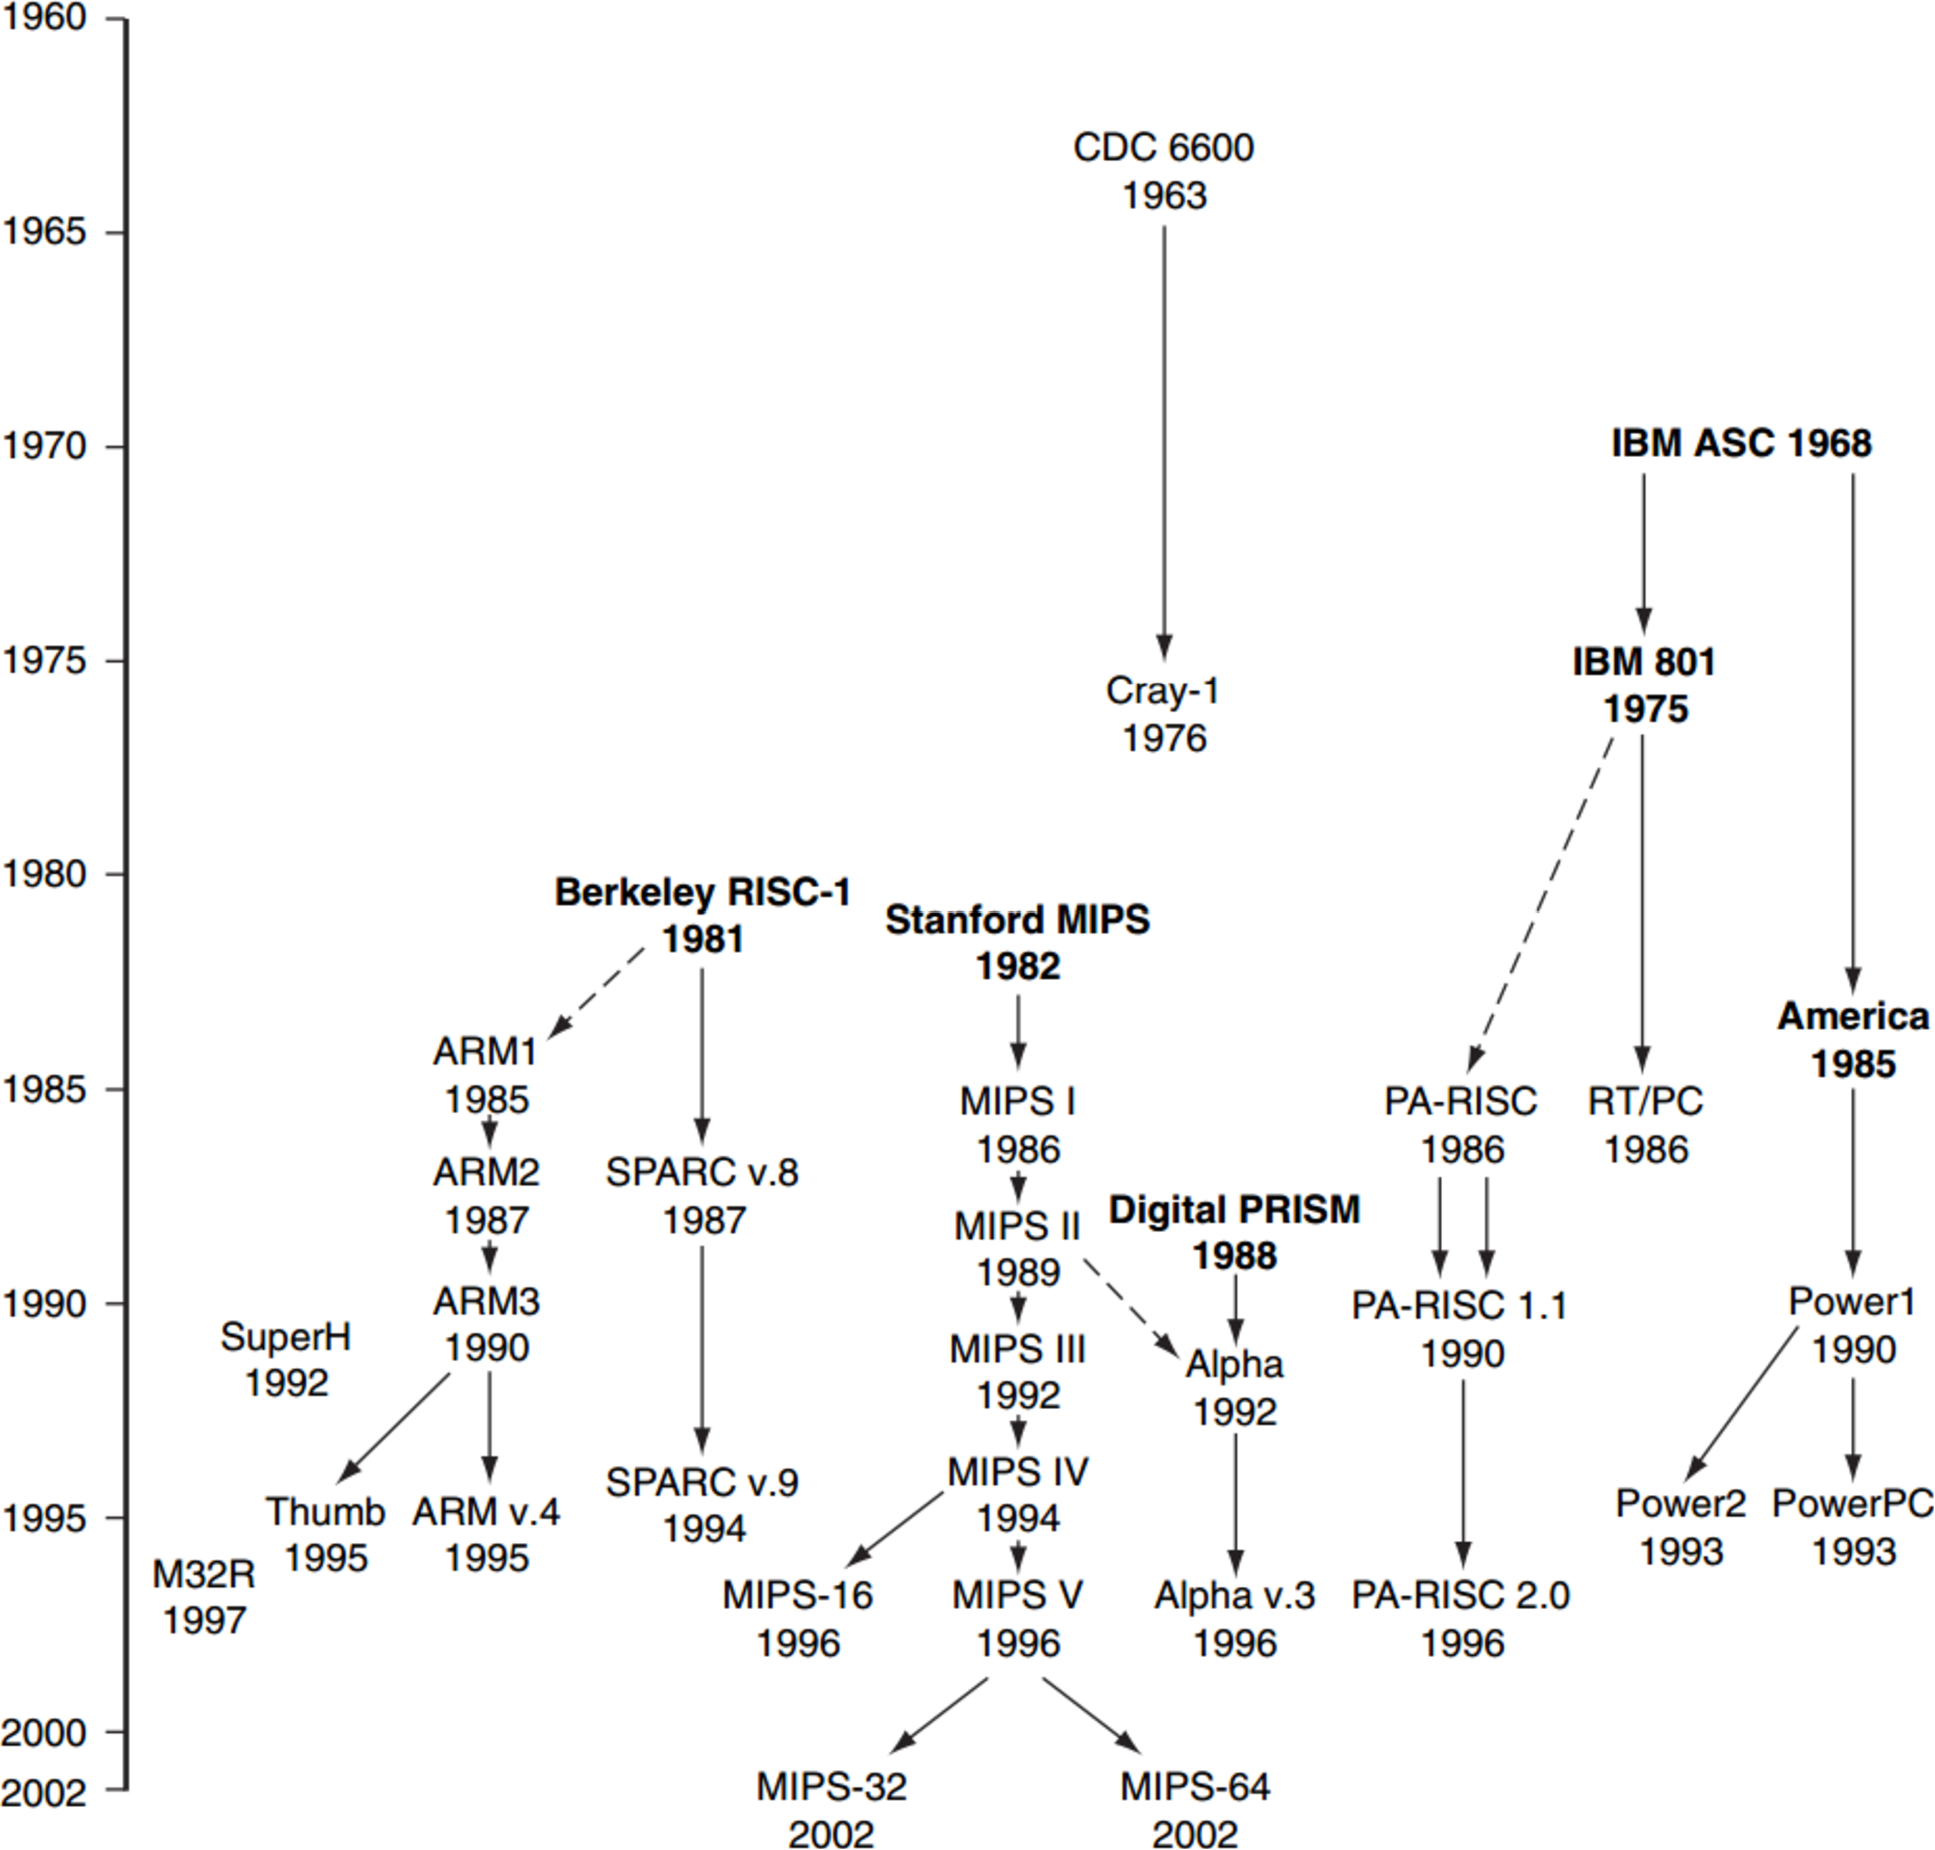
\includegraphics[width=0.7\textwidth]{fig/c1_introducao/history_risc.pdf}
\caption{Linha do tempo das arquiteturas RISC, extraido de \cite{Hennessy2011}. Em negrito estão as iniciativas de pesquisa, em contraste às comerciais.}
\label{fig:history_risc}
\end{figure}

Por volta dos anos 2000, a pot\^encia dissipada em cada transistor, proporcional a frequência de opera\c{c}\~ao, havia atingido o limite suportado pelo microprocessador.
Por causa disso, o crescimento desenfreado da frequ\^encia teve que ser repensado.
Come\c{c}ou-se ent\~ao o desenvolvimento de microprocessadores \textit{multicore}, que aumentam a vaz\~ao de instru\c{c}\~oes (\textit{throughtput}) sem modificar o tempo de resposta, que corresponde ao tempo de processamento médio de uma instrução.
Em meados de 2006, todas as grandes companhias j\'a possuiam produtos com esta arquitetura \cite{Hennessy2011}.

Os microprocessadores com v\'arios n\'ucleos (\textit{multicore}) abriram espa\c{c}o para a chegada de processadores com muitos n\'ucleos (\textit{manycore}).
Estes microprocessadores s\~ao projetados para placas gr\'aficas e, apesar de possuirem centenas de n\'ucleos, estes núcleos s\~ao simplificados \cite{Vajda2011}.
Em geral, eles são capazes de realizar apenas algumas poucas operações, mas abrem caminho para paradigmas de programação que transformem a computação concorrente em computação paralela \cite{Harel2004}.

Mesmo trabalhando com um ou v\'arios n\'ucleos de processamento, o modelo de computa\c{c}\~ao atual ainda \'e dito temporal ou sequencial uma vez que blocos de instru\c{c}\~oes s\~ao executados em seu devido instante de tempo de forma sequencial, conceito destacado pela atomicidade estudada em programa\c{c}\~ao paralela \cite{williams2012c++}.

Do ponto de vista da programa\c{c}\~ao, os primeiros computadores apresentavam programas que n\~ao podiam ser alterados.
Parte desta limita\c{c}\~ao era justificada pela programa\c{c}\~ao utilizando-se cart\~oes, mas nas primeiras gera\c{c}\~oes de computadores com mem\'orias eletr\^onicas o mesmo sistema foi utilizado.

A arquitetura de von Neumann, utilizada na primeira gera\c{c}\~ao de computadores eletr\^onicos, era cons\-ti\-tu\'i\-­da de uma \'unica unidade de mem\'oria, uma unidade de processamento e um canal de comunica\c{c}\~ao.
Esta arquitetura possui tanto uma vantagem tremenda, a capacidade de modifica\c{c}\~ao de programas em tempo de execu\c{c}\~ao, quanto uma falha crucial, conhecida por gargalo de von Neumann.
A vantagem aparece uma vez que, como n\~ao h\'a distin\c{c}\~ao entre mem\'oria de programa e dados, uma instru\c{c}\~ao pode sobrescrever um endere\c{c}o de mem\'oria marcado como programa.
O problema diz respeito \`as restri\c{c}\~oes impostas pelo canal de comunica\c{c}\~ao, que permitia que apenas uma palavra, seja de programa ou de dados, fosse mandada para a unidade de processamento e de volta \cite{Backus1978}.
Este problema se agrava a medida que o processador fica mais r\'apido que a mem\'oria, uma vez que o tempo de espera, em ciclos de rel\'ogios, para a obten\c{c}\~ao da informa\c{c}\~ao aumenta.
Para solucionar o problema do gargalo de von Neumann, a arquitetura Harvard foi proposta.

A arquitetura Harvard original propunha que a mem\'oria de programa e a mem\'oria de dados fossem fisicamente separadas e possuissem cada uma seu pr\'oprio canal de comunica\c{c}\~ao com o processador \cite{Hennessy2011}.
Essa modifica\c{c}\~ao acelera a execu\c{c}\~ao de certos programas, visto que programa e dados podem ser carregados das suas respectivas mem\'orias simultaneamente.
Uma pequena altera\c{c}\~ao na arquitetura Harvard, conhecida de arquitetura Harvard modificada, permitia que mais de um canal de comunica\c{c}\~ao ligasse a uma mem\'oria tanto de programa quanto de dados \cite{Hennessy2011}.
Essas informa\c{c}\~oes eram divididas em mem\'orias tempor\'arias (\textit{cache}) espec\'i­ficas para o programa e para dados, formando assim uma arquitetura Harvard original.
Essa modifica\c{c}\~ao combina os benef\'i­cios da arquitetura de von Neumann, ou seja, a modifica\c{c}\~ao de programas em tempo de execu\c{c}\~ao, e da arquitetura Harvard original, ou seja, o tempo de acesso reduzido.

Atualmente, nossos modernos computadores multiprocessados utilizam a arquitetura Harvard modificada com diversos n\'i­veis de mem\'oria \textit{cache} \cite{Hennessy2011}, sejam eles dedicados ou compartilhados entre os v\'arios processadores.
A sua capacidade de processamento atinge n\'i­veis extraordin\'arios, ultrapassando 20 GFlops em computadores comuns \cite{MaxxPI2013} e 54 PFlops em supercomputadores \cite{Top5002013}.
Apesar disso, a arquitetura Harvard original ainda \'e muito usada em microcontroladores e processadores digitais de sinal (\textit{Digital Signal Processors} ou DSPs).

\section*{Computa\c{c}\~ao Reconfigur\'avel}
\label{ss:computacao_reconfiguravel}
A computa\c{c}\~ao reconfigur\'avel foi proposta por volta de 1960 por Gerald Estrin para resolver problemas que n\~ao podiam ser resolvidos pela computa\c{c}\~ao da \'epoca \cite{Estrin2002}.
Estrin prop\^os um microprocessador composto de uma parte fixa e uma parte vari\'avel, onde a parte vari\'avel seria usada para programar funcionamentos espec\'i­ficos para serem usados em determinados per\'i­odos de tempo.
%A id\'eia de Estrin foi deixada de lado \`a medida que os microprocessadores e \textit{Application-Specific Integrated Circuits} (ASICs) se mostraram aptos a resolver os problemas da \'epoca.
Por volta da d\'ecada de 1990, por\'em, o primeiro microprocessador h\'i­brido comercial foi desenvolvido \cite{Estrin2002}, trazendo esta tecnologia \`a tona.

A tecnologia inventada por Estrin, tamb\'em conhecida como estrutura \textit{Fixed Plus Variable} (F+V), cuja representação está mostrada na figura \ref{fig:model_f+v}, trouxe \`a tona um novo paradigma de processamento de dados \cite{Hartenstein2001}.
O motivo para tal \'e o fato de que a intera\c{c}\~ao entre as unidades de processamento e os dados mudou completamente.
O que antes se conhecia por modelo temporal de computa\c{c}\~ao foi deixado de lado para, nesta nova arquitetura, se tornar um modelo espacial.
Em outras palavras, os dados n\~ao eram direcionados um a um para uma unidade central de processamento, mas processados continuamente em um sistema distribu\'i­do no espa\c{c}o \cite{vassiliadis2007fine}.
Tal sistema distribu\'i­do \'e composto de c\'elulas l\'ogicas e suas conex\~oes, ambas reprogram\'aveis, ajudando a se alcan\c{c}ar uma efici\^encia similar a presente em ASICs e flexivel como a computa\c{c}\~ao gen\'erica.

\begin{figure}[h]
\centering
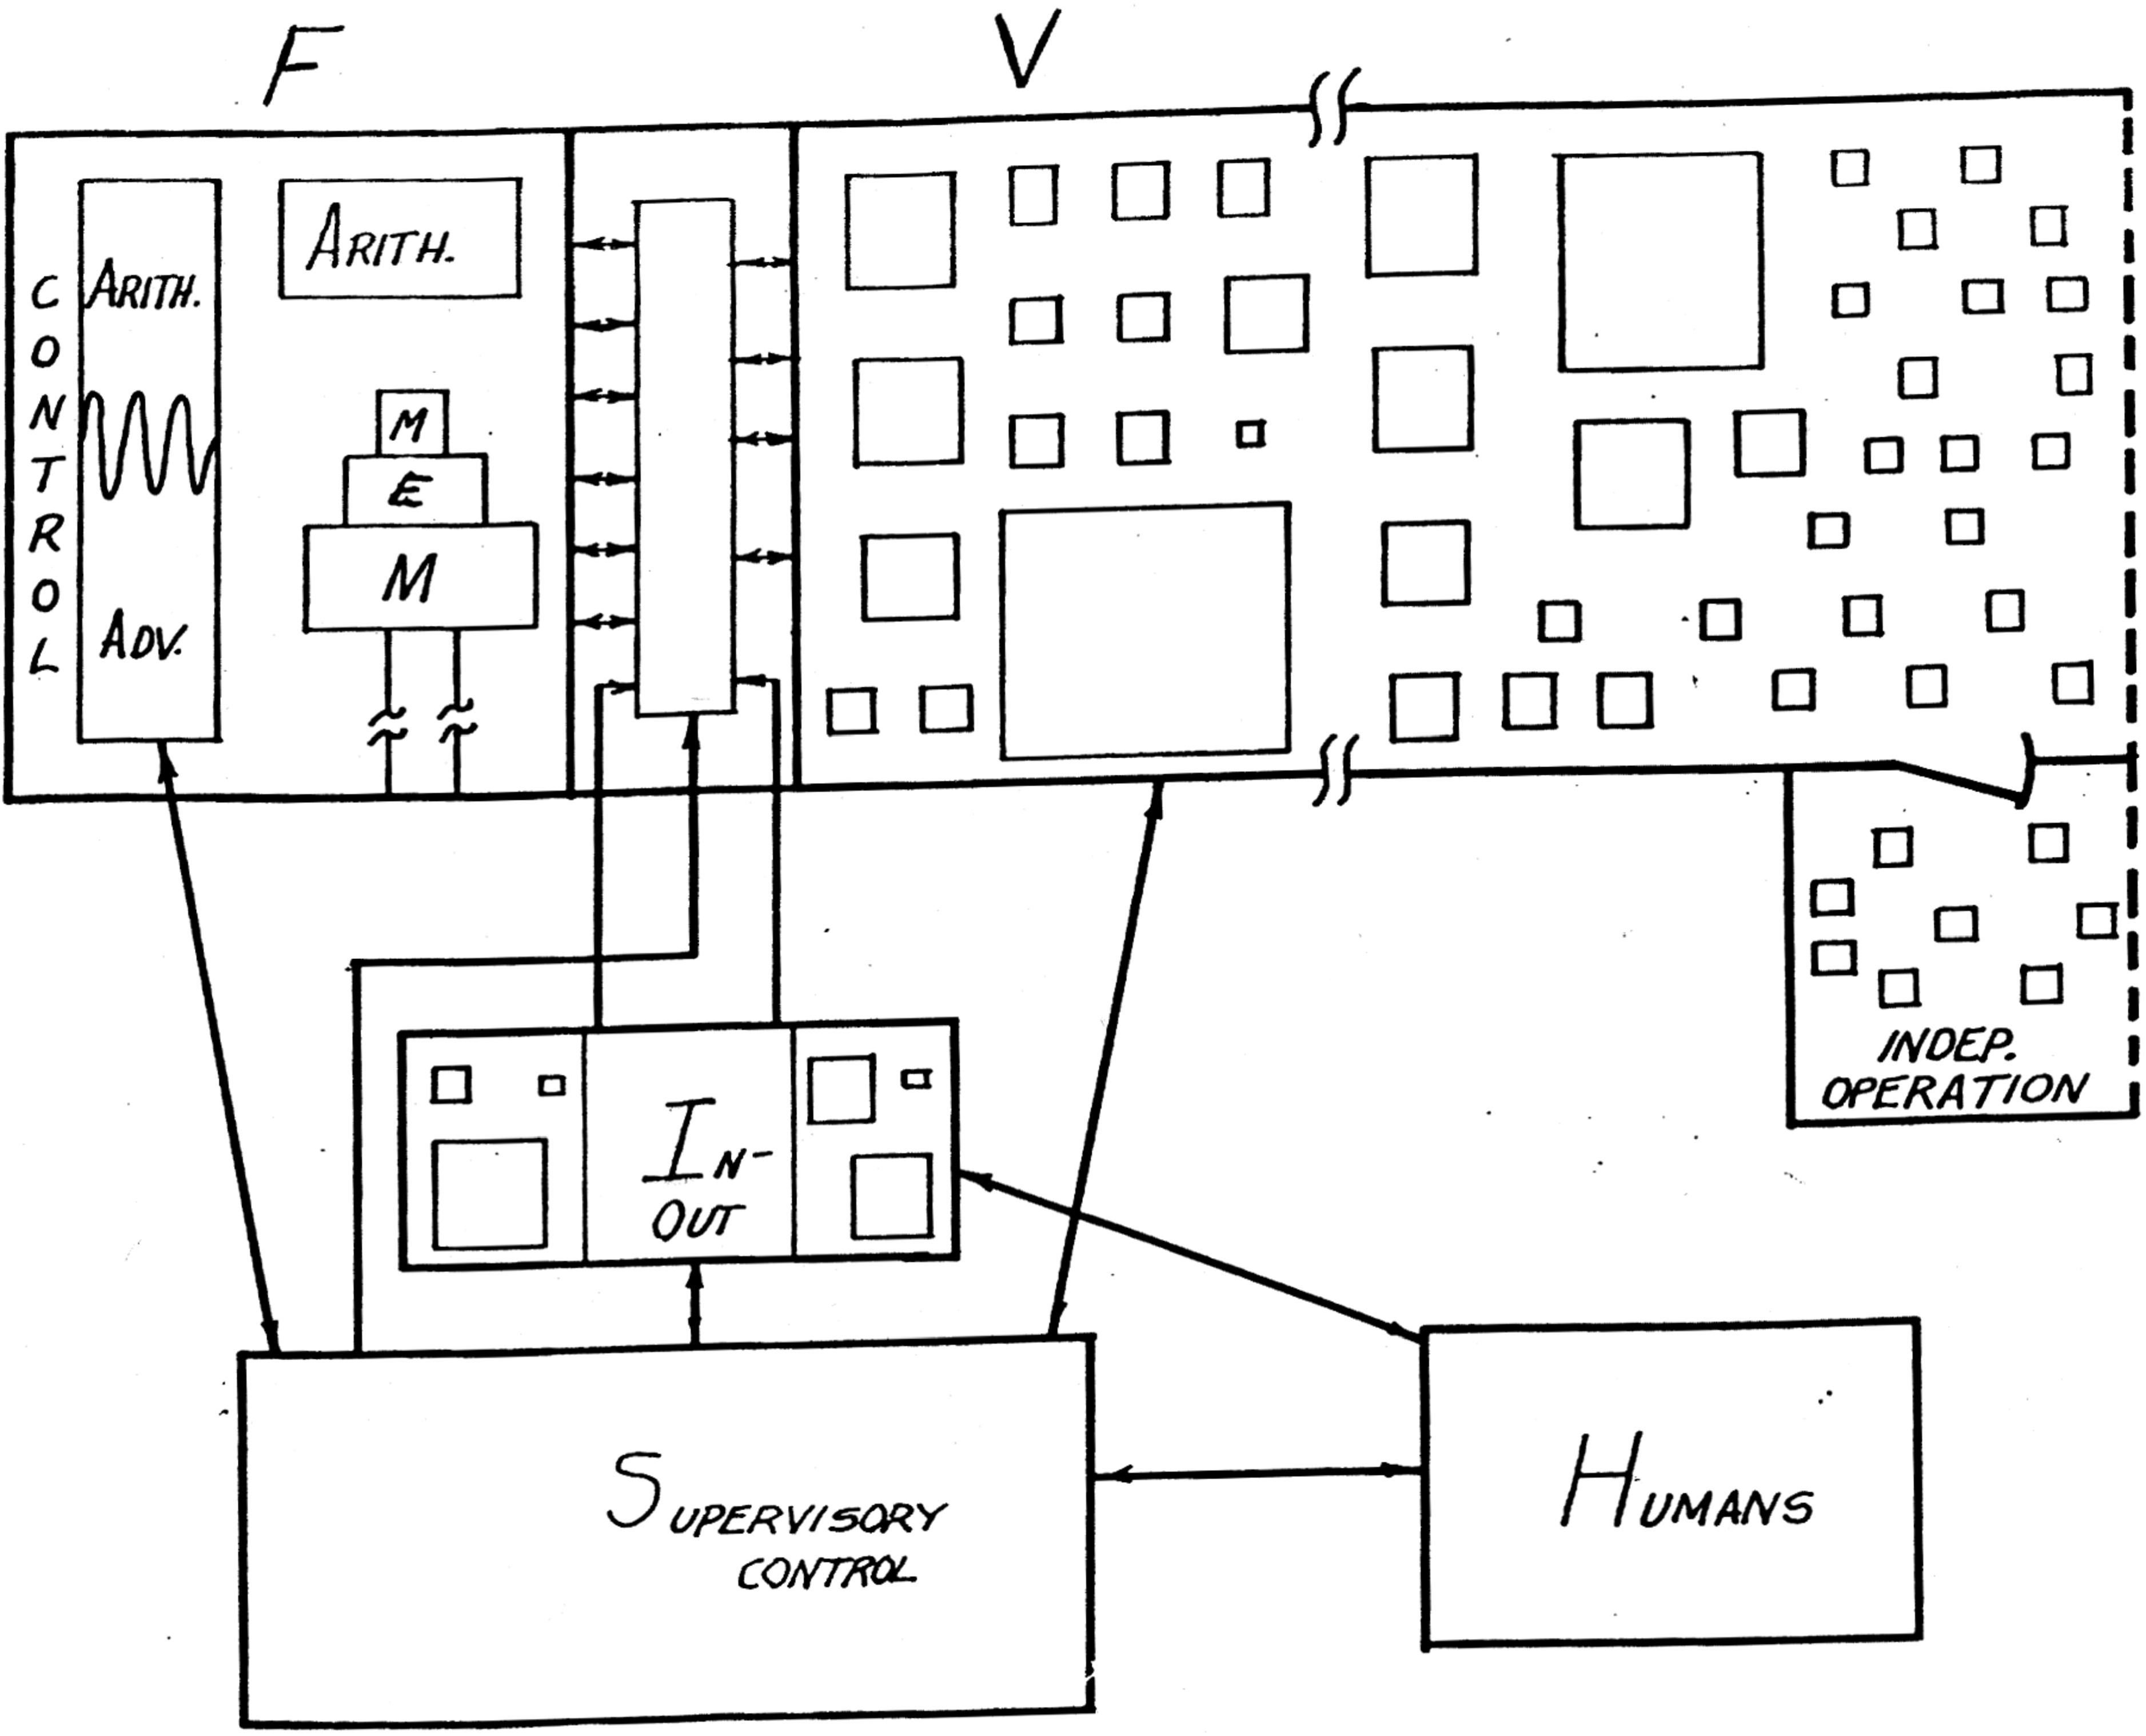
\includegraphics[width=0.7\textwidth]{fig/c1_introducao/model_f+v.pdf}
\caption{Esquem\'atico com o F+V, extraido de \cite{Estrin2002}.}
\label{fig:model_f+v}
\end{figure}

Ao contr\'ario da estrutura F+V proposta por Estrin, a maioria dos sistemas reconfigur\'aveis atuais possuem apenas a parte reconfigur\'avel.
Apesar de sistemas reconfigur\'aveis de alta performance possuirem componentes fixos como processadores e unidades de processamento gr\'aficos (GPUs) \cite{El-Ghazawi2008}, a sua aus\^encia reduz o custo de projeto e a flexibilidade do projeto final.

Os sistemas reconfigur\'aveis atuais utilizam de tr\^es meios principais de programa\c{c}\~ao: \textit{Static Random-Access Memory} (SRAM), \textit{Antifuse} e mem\'orias n\~ao-vol\'ateis.
Usando SRAM, o resultado da s\'i­ntese
%, processo comentado na se\c{c}\~ao \ref{sss:sintese},
 \'e armazenado nas c\'elulas desta mem\'oria e controlam o estado dos transistores das c\'elulas l\'ogicas.
No caso de c\'elulas compostas de tabelas de busca (\textit{look-up tables} ou LUTs), a SRAM armazena os dados dessas c\'elulas.
Outra segunda tecnologia de programa\c{c}\~ao, o \textit{antifuse}, faz uso de uma conex\~ao com imped\^ancia vari\'avel, onde atrav\'es do uso de altas voltagens pode-se modificar a resist\^encia de uma via.
Esse processo de programa\c{c}\~ao \'e irrevers\'i­vel.
As mem\'orias n\~ao vol\'ateis, como EPROM, EEPROM e FLASH, usam transistores especiais com uma ponte flutuante.
Quando a ponte possui carga, o transistor pode ser controlado pela ponte de sele\c{c}\~ao, que permanece carregada at\'e quando desligada.
Estas t\'ecnicas permitem a resist\^encia da \textit{antifuse} e a reprogramabilidade da SRAM, sendo apenas mais complexa e demorada para ser programada \cite{vassiliadis2007fine}.

As interconex\~oes entre c\'elulas l\'ogicas, que influenciam diretamente as c\'elulas em si, podem ser de cinco tipos: ilha, linha, mar-de-portas, hier\'arquico e estruturas unidimensionais \cite{vassiliadis2007fine}.
A arquitetura do tipo ilha consiste em c\'elulas l\'ogicas conectadas umas as outras atrav\'es de caixas de conex\~oes e de roteamento.
Nesta arquitetura, a c\'elula l\'ogica est\'a cercada por trilhas de conex\~oes, o que explica o nome.
A arquitetura do tipo linha consiste em v\'arias linhas divididas em quantidades variadas de segmentos.
As conex\~oes s\~ao ent\~ao realizadas usando-se linhas verticais atrav\'es de blocos l\'ogicos especiais.
A arquitetura do tipo mar-de-portas consiste de blocos l\'ogicos que cobrem todo o espa\c{c}o do dispositivo e s\~ao conectados aos seus vizinhos diretos.
Em geral este tipo de conex\~ao \'e mais r\'apido.
A arquitetura do tipo hier\'arquico agrupa as c\'elulas l\'ogicas em \textit{clusters}, e agrupa estes em \textit{clusters} de mais alto n\'i­vel, formando de fato um sistema hier\'arquico.
O \'ultimo tipo de arquitetura, unidimensional, surge como uma tentativa de simplificar o roteamento complexo dos sistema bidimensionais apresentados anteriormente.
Nele, restri\c{c}\~oes de aloca\c{c}\~ao e roteamento s\~ao impostas para reduzir o n\'umero de possibilidades.
O problema deste tipo de arquitetura \'e que se n\~ao houverem recursos de roteamento suficientes, o roteamento fica mais complexo que nas arquiteturas bidimensionais.

As arquiteturas reconfigur\'aveis podem ser classificada em tr\^es tipos segundo a granularidade.
A granularidade diz respeito a quantidade de informa\c{c}\~ao m\'i­nima que pode ser passada de uma c\'elula l\'ogica para outra.
Ela separa as arquiteturas reconfigur\'aveis em tr\^es categorias: granularidade fina, grossa e h\'i­brida.
Nas arquiteturas com granularidade fina, como os \textit{Field-Programmable Gate Arrays}, um \'unico \textit{bit} pode ser transferido de uma c\'elula a outra, permitindo assim um maior controle sobre os dados.
Nas arquiteturas com granularidade grossa, os \textit{bits} s\~ao agrupados em palavras de tamanhos fixos, reduzindo assim o espa\c{c}o gasto com roteamento e melhorando a roteabilidade \cite{Hartenstein2001}.
No \'ultimo tipo de arquiteturas, a h\'i­brida, parte das conex\~oes s\~ao grossas e partes s\~ao finas, combinando os benef\'i­cios das duas classes.

\section{Motivação}
A reconfiguração dinâmica, bem como a autorreconfiguração, tem aplicação em diversas áreas.
Esta seção apresenta uma série de propostas de aplicação da tecnologia.

\subsection{Tolerância a Falhas}
Muitas aplicações possuem como requisito a tolerância a falhas.
Em geral, seu funcionamento é crítico e pode incorrer em grandes prejuízos financeiros, na morte de pessoas ou mesmo na correta realização de um experimento.
Alguns exemplos destas aplicações são o controle de um equipamento industrial, o controle de um avião e o controle ou tratamento de dados de um sistema espacial respectivamente.
Os dispositivos nestas aplicações podem ter seu funcionamento comprometivo devido a temperatura do ambiente (quente ou frio), impactos, descargas elétricas não-intencionais e/ou radiação.

Em geral, a robustez a falhas é realizada através da redundância de equipamentos, permitindo a troca quando se percebe que algum componente falhou.
Esta prática possui um grave problema, que diz respeito ao gasto exagerado de dinheiro.
A reconfiguração dinâmica e a autorreconfiguração podem ser utilizados para reduzir estes gastos, que podem chegar a várias vezes o preço do projeto original.

Em sistemas reconfiguráveis, existem algumas formas diferentes de se garantir a tolerância a falhas, que em geral variam de acordo com a aplicação.
A mais comum delas é a verificação da configuração deste dispositivo.
Existem ainda forma de verificar a vazão de dados, a corretude destes dados, entre outros.

Na verificação da configuração, utiliza-se de ferramentas para leitura da configuração atual do dispositivo e a comparação desta com a configuração original armazenada em alguma memória mais confiável.
Este processo por vezes é otimizado calculando-se um valor estatisticamente único para aquela configuração através de uma função de \textit{hashing}.
A mudança de apenas um bit na configuração é suficiente para modificar bastante o valor de \textit{hash}, como é conhecido a saída da função de \textit{hashing}, fornecendo assim uma forma mais eficiente, devido a drástica redução no tamanho da informação utiilzada, e igualmente eficaz de se verificar alterações indesejadas na configuração do dispositivo.
Após idenficada a falha, é possível reprogramar o dispositivo, modificar a partição onde o seu comportamento tinha sido configurado ou mesmo sinalizar a um operador a necessidade de manutenção.

\subsection{Redes Neurais}
Redes neurais s\~ao uma ferramenta de inteligência artificial largamente utilizada nas \'areas de \textit{Data Mining} e sistemas que necessitem de algum tipo de aprendizado.
Elas utilizam de redes de elementos extremamente simples, como mostrado na figura \ref{fig:nn}, para criar uma fun\c{c}\~ao altamente n\~ao-linear com um comportamento esperado.
Estes elementos podem ser matematicamente representados por somat\'orios ponderados afunilados por fun\c{c}\~oes n\~ao-lineares.
Os pesos utilizados nestes somat\'orios s\~ao os elementos a serem adaptados de forma a modificar o comportamento da estrutura.
Elas podem ser utilizadas tanto aprendizados supervisionados, onde funciona como um poderoso aproximador de fun\c{c}\~oes, quanto em aprendizados n\~ao-supervisionados, onde traduz um sistema hiperdimensional em bidimensional.

\begin{figure}[h]
\centering
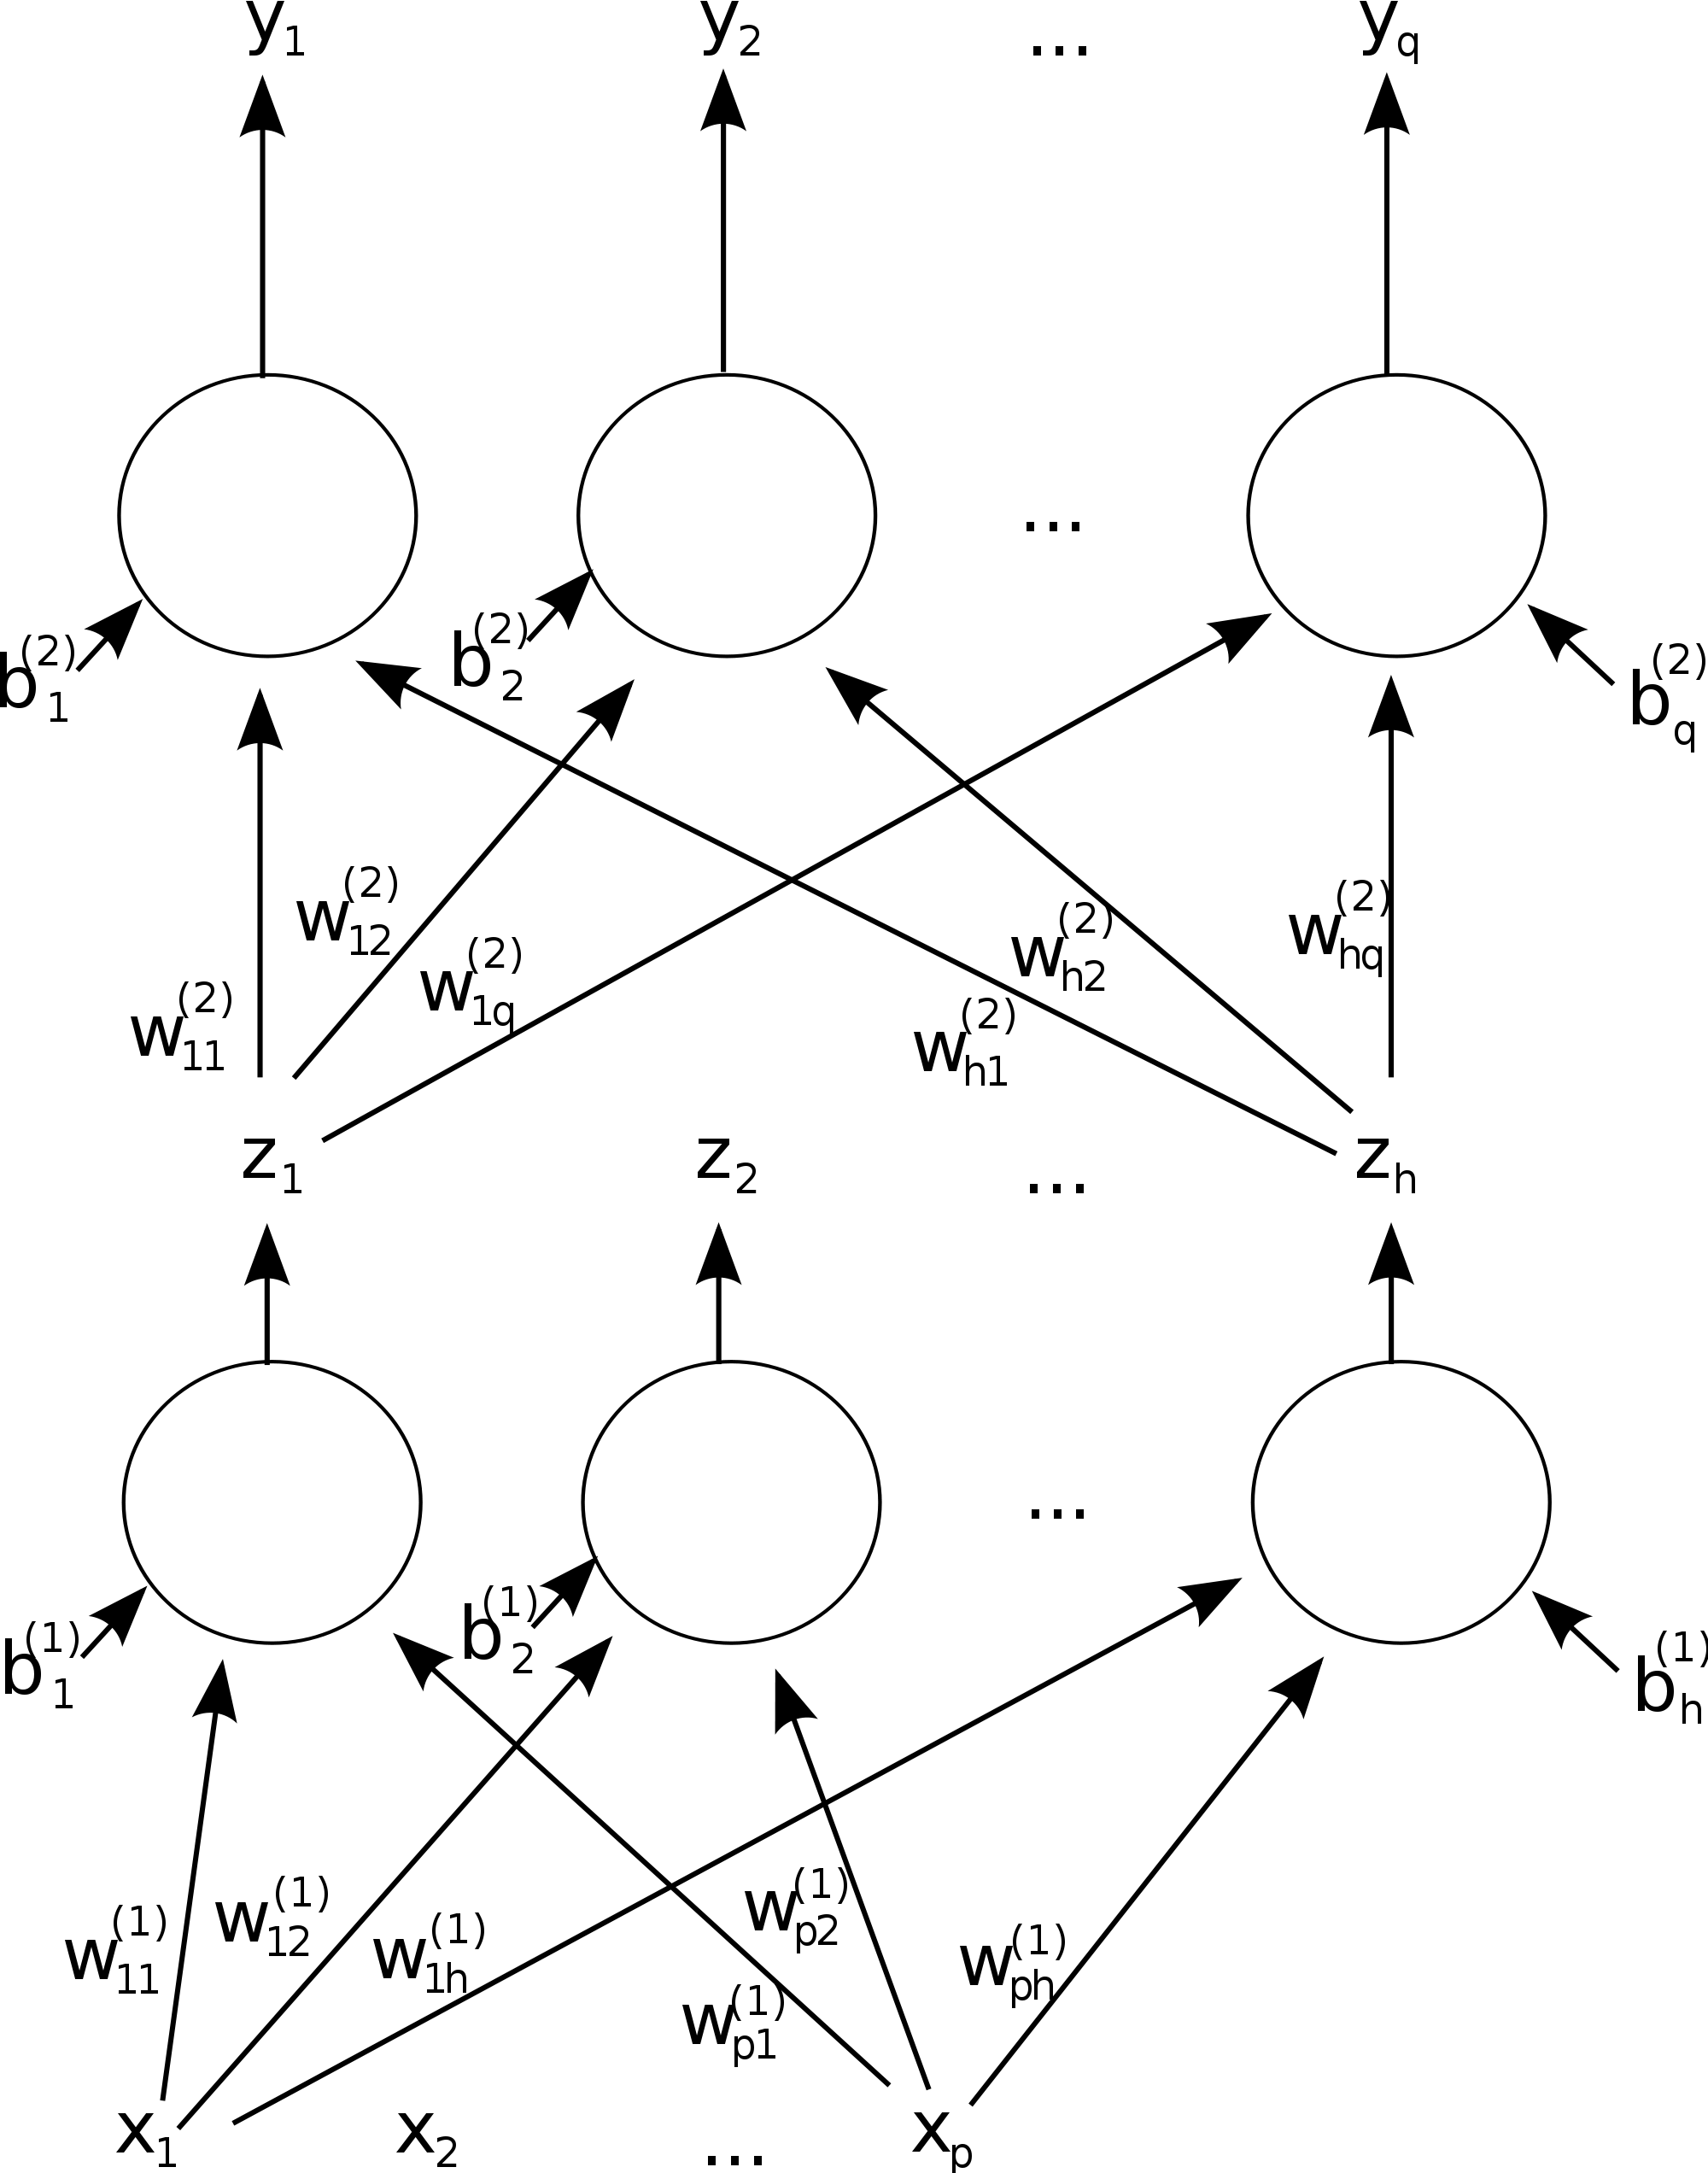
\includegraphics[width=0.5\textwidth]{fig/propostas/model_nn}
\caption{Modelo de rede neural com "$p$" entradas, "$q$" saídas e duas camadas.}
\label{fig:nn}
\end{figure}

As redes neurais podem possuir v\'arias camadas de neur\^onios, que s\~ao as unidades b\'asicas de processamento, e v\'arias entradas e saídas.
Quanto mais camadas s\~ao acrescentadas ao sistema, mais inst\'avel fica seu treinamento e custosa sua computa\c{c}\~ao.
Em geral utilizam-se apenas duas ou três camadas com um n\'umero arbitr\'ario de neur\^onios em cada uma.
N\~ao existe um algoritmo que determine qual seria a topologia ideal de uma rede para um certo modelo.
Tal decis\~ao normalmente \'e feita com base em experiência e tentativas e erros.

Existem topologias três topologias b\'asicas de redes neurais: a \textit{feedforward}, a recorrente e a atrasada.
A primeira possui neur\^onios que entregam seus resultados apenas para camadas mais a frente.
A segunda, mais complexa, al\'em de entregar seus resultados para as camadas mais a frente, realimentam camadas anteriores.
A \'ultima utiliza de elementos especiais para atrasar o uso de certas entradas ou resultados.

As redes neurais podem ser usadas de diversas formas diferentes: atrav\'es de treinamento \textit{online}, onde o sistema continuamente recebe informa\c{c}\~oes e treina os pesos dos seus neuronios; atrav\'es de treinamento em lotes, onde o sistema acumula um lote de informa\c{c}\~oes e treina o sistema lote a lote; atrav\'es de treinamento \textit{offline}.
Cada um dos usos listados tem seu uso específico e suas vantagens e desvantagens.
O treinamento \textit{online} tem a vantagem de se adaptar mais frequentemente ao sistema que tenta modelar, mas precisa de muito mais processamento/potência para manter o sistema treinado.
O treinamento em lotes tem a vantagem de poder ter a frequência de atualiza\c{c}\~ao dos pesos modificada de acordo com as necessidades.
Sendo assim, a rela\c{c}\~ao taxa de atualiza\c{c}\~ao/potência pode ser ajustada.
O treinamento \textit{offline} tem a vantagem de considerar um conjunto potencialmente representativo do sistema modelado al\'em da vantagem de ser a forma que precisa de menos processamento, visto que a atualiza\c{c}\~ao dos pesos acontece apenas uma vez.
A desvantagem dessa forma \'e a falta de capacidade de adapta\c{c}\~ao frente a sistemas vari\'aveis no tempo.

Al\'em das formas de funcionamento das redes neurais, outra característica que a define grandemente \'e o algoritmo de treinamento utilizado.
Dentre os mais populares existem o \textit{backpropagation} e o de Levenberg-Marquardt.
O algoritmo de \textit{backpropagation} \'e o mais difundido devido a sua facilidade de entendimento e implementa\c{c}\~ao.
J\'a o algoritmo de Levenberg-Marquardt vê o ajuste de pesos de uma rede neural como um problema de otimiza\c{c}\~ao.

A computa\c{c}\~ao reconfigur\'avel, mais especificamente a reconfigura\c{c}\~ao dinâmica parcial, pode ser usada para modificar a topologia da rede neural.
Ela pode ser programada para, quando o erro ultrapassar um certo limite m\'aximo, aumentar ou diminuir o n\'umero de neur\^onios numa certa camada.
Os desafios referentes a essa proposta s\~ao apenas relacionados a implementa\c{c}\~ao de um sistema com reconfigura\c{c}\~ao dinâmica parcial.

Uma outra possibilidade \'e a modifica\c{c}\~ao do algoritmo de treinamento com base em seus custos computacionais e erros.
Quando um algoritmo de baixo custo computacional come\c{c}ar a retornar um erro acima de certo limite m\'aximo, ele seria trocado pelo algoritmo imediatamente mais custoso.
Os desafios dessa proposta s\~ao, al\'em dos relacionados a implementa\c{c}\~ao de um sistema com reconfigura\c{c}\~ao dinâmica parcial, a implementa\c{c}\~ao em \textit{hardware} de algoritmos de treinamentos de redes neurais.

Ainda outra possibilidade seria a de implementar uma autorreconfigura\c{c}\~ao n\~ao-planejada no sistema, onde o n\'umero de neur\^onios e a forma de suas conex\~oes n\~ao seriam programados previamente em configura\c{c}\~oes específicas, como na primeira proposta, mas determinados em tempo de execu\c{c}\~ao.
De forma um pouco mais clara, apenas o comportamento e \textit{bitstreams} referentes aos elementos b\'asicos/neur\^onios seriam programados.
Suas conex\~oes e pesos seriam determinados por um sistema controlador presente na l\'ogica est\'atica do sistema reconfigur\'avel.
A dificuldade de implementa\c{c}\~ao desse projeto o torna invi\'avel para um trabalho deste porte.

\subsection{Controle Adaptativo}
O controle adaptativo tradicional tem como principal objetivo o controle de sistemas incertos ou com características variantes no tempo.
Um controlador adaptativo tem a forma mostrada na figura \ref{fig:cadapt}.
Este sistema implementa uma l\'ogica de estima\c{c}\~ao e corre\c{c}\~ao de parâmetros segundo a estabilidade de Lyapunov.

\begin{figure}[h]
\centering
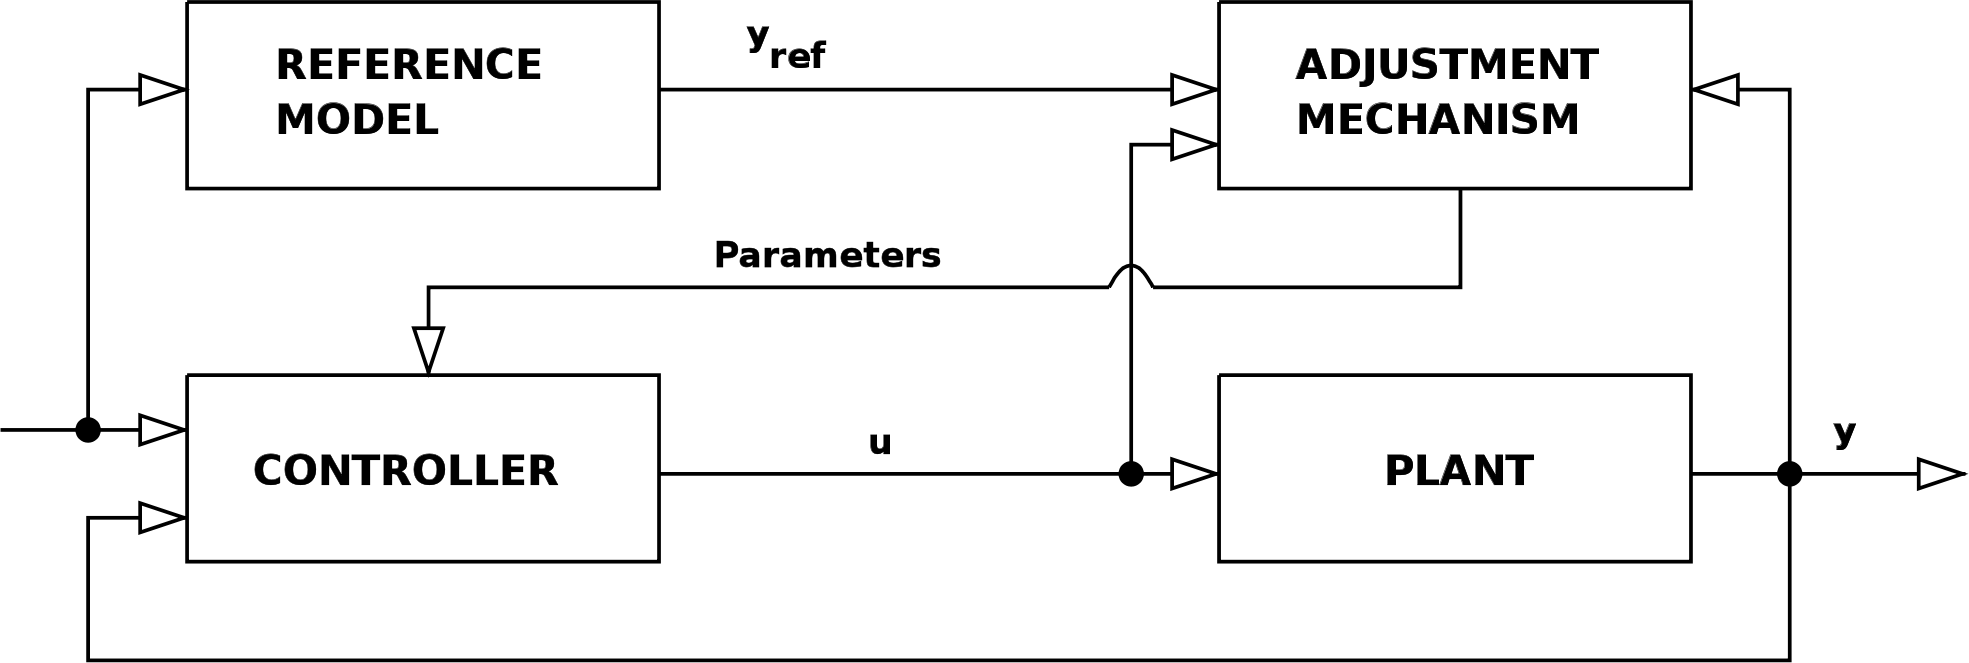
\includegraphics[width=0.8\textwidth]{fig/propostas/model_MRAC}
\caption{Modelo de um controlador adaptativo do tipo MRAC.}
\label{fig:cadapt}
\end{figure}

Utilizando o conceito básico deste tipo de controle e a reconfiguração dinâmica, é possível construir um controlador cuja forma é mudada segundo os requisitos dos sistema, i.e. hora seria um controlador proporcional, hora seria um controlador proporcional-integral-derivativo.
As dificuldades desta proposta dizem respeito implementa\c{c}\~ao de sistemas com reconfigura\c{c}\~ao dinâmica parcial e ao projeto do sistema que controlaria a troca entre controladores.

\subsection{Computação Genérica}
Um computador de computação genérica possui um conjunto fixo de instruções implementados em um sistema imutável no tempo.
A figura \ref{fig:mips} apresenta um processador MIPS de 5 estágios representando este um processador comum, i.e. imutável.
Os únicos elementos lógicos passíveis de alteração são as memórias.

\begin{figure}[h]
\centering
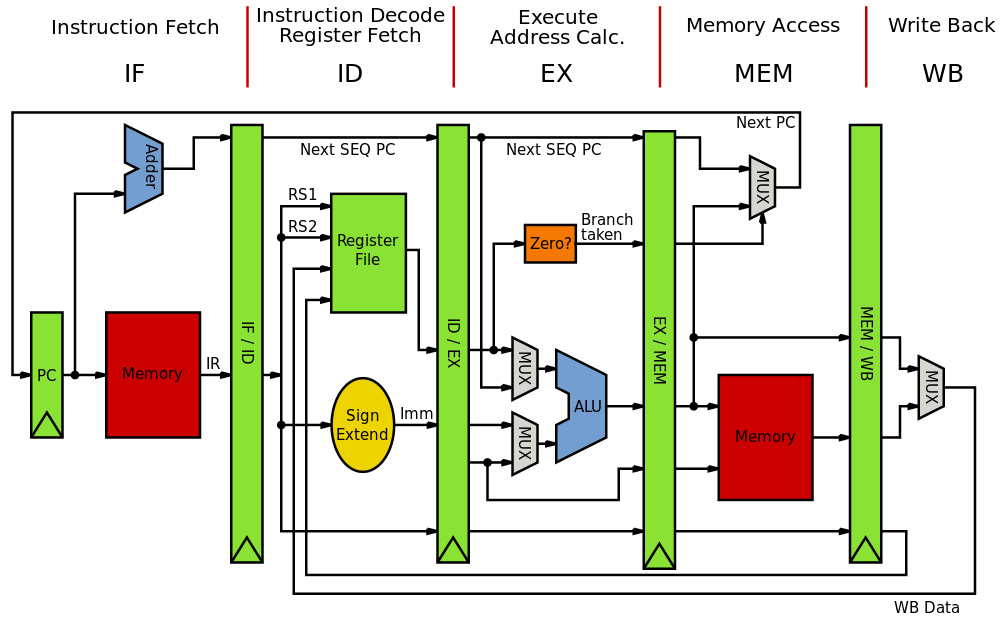
\includegraphics[width=0.8\textwidth]{fig/propostas/MIPS_Architecture_(Pipelined)}
\caption{Ilustração de um processador MIPS com \textit{pipeline} de 5 estágios.}
\label{fig:mips}
\end{figure}

O uso de autorreconfiguração este caso possibilitaria a redução do espaço físico necessário para a implementação de elementos da unidade de lógica e aritmética (ALU).
Esta modificação permitiria também uma diminuição no consumo de energia do processador, além de permitir que instruções de ponto flutuante fossem implementadas diretamente na ALU, sem a necessidade de extensão do processador.
Outra possibilidade é a implementação de um banco de registradores variável, permitindo ao compilador escolher quantos registradores utilizar em cada etapa do seu programa, otimizando ainda mais o desempenho deste.

As dificuldades deste projeto dizem respeito a necessidade de construção prévia de um processador genérico funcional, a incluisão de uma memória para armazenamento de configurações, o desenvolvimento de cada configuração parcial para este componente e o desenvolvimento de um controlador para a troca de configurações.
É provável que o circuito responsável pela reconfiguração possa ganhar um estágio dedicado a ele, devivo a sua complexidade e ao tempo de programação.
Para se contornar o problema do tempo de reconfiguração, pode-se utilizar diversas ALUs, onde apenas uma estaria ativa no ciclo em execução.
Sendo assim, outros sistemas de controle podem ser necessários.

Uma outra possibilidade de implementação, menos eficiente, é a reconfiguração do sistema estágio-a-estágio.
Ou seja, quando o dispositivo fosse ligado, apenas o primeiro estágio estaria programado.
Esta implementação não é recomendada, uma vez que transforma um processador com \textit{pipeline} em um processador uniciclo.

\subsection{Outros}
De forma geral, qualquer sistema multiplexado ou que possua diversas etapas de processamento, pode ser implementado utilizando-se de autorreconfiguração.
Deve-se, porém, para sua utilização em aplicações reais, verificar se o \textit{overhead} de tempo introduzido é balanceado pelos ganhos de performance e potência.

\section{Objetivos}
\subsection{Objetivos Gerais} Estudar o fluxo de projeto da reconfiguração dinâmica e da autorreconfiguração.

\subsection{Objetivos Específicos}
Como mostrado na figura \ref{fig:objetivos}, este projeto foi estruturado de forma a se desenvolver o estudo proposto de forma lógica, fluida e incremental.

Como o objetivo final é a familiarização com as ferramentas e processos envolvidos na autorreconfiguração, decidiu-se começar estudando os elementos necessários para se realizar a reconfiguração dinâmica.
O passo seguinte mais lógico é o de estudar como funciona as memórias dos sistema e de que jeito elas seriam melhor utilizadas.
O último passo seria entender como funciona a autorreconfiguração em baixo nível, ou seja, como os dados devem ser entregues aos devidos componentes para que ela aconteça.
Para cada um destes experimentos foi proposto um teste que validasse o completo entendimento do mesmo.

\begin{figure}[h]
\centering
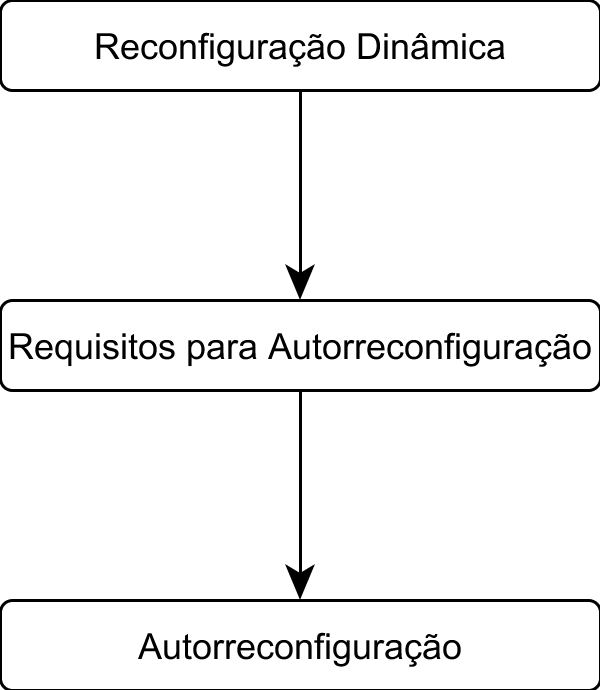
\includegraphics[width=0.35\textwidth]{fig/c1_introducao/objetivos}
\caption{Ilustração de um processador MIPS com \textit{pipeline} de 5 estágios.}
\label{fig:objetivos}
\end{figure}

\paragraph{Verificar visualmente a ocorrência da reconfiguração dinâmica:} A visualização desta tecnologia constitui a prova necessária para a validação do projeto proposto.
Este objetivo visa o entendimento da forma mais básica de reconfiguração dinâmica, permitindo assim que os detalhes mais importantes da sua implementação sejam percebidos e considerados na formulação de experimentos.

\paragraph{Entender e estudar detalhadamente os requisitos para a construção de um sistema autorreconfigurável:} Entende-se que existem alguns requisitos para a autorreconfiguração que não são completamente claros. Após sua identificação, pretende-se estudar como eles funcionam e como utilizá-los em um projeto simplificado.

\paragraph{Implementar um sistema autorreconfigurável:} Este trabalho deverá culminar no entendimento e implementação de um sistema autorreconfigurável simples. Para tal, espera-se que se entenda completamente o fluxo de projeto deste tipo de sistemas e as peculiaridades da sua implementação.

\section{Experimentos/Metodologia}
Como foi mencionado na seção anterior, este trabalho utilizará experimentos para auxiliar o desenvolvimento do estudo proposto.
Desta forma, além de garantir algum material mesmo que tudo dê errado, consegue-se simplificar o processo de pesquisa e desenvolvimento através dos pequenos passos e análises frequentes.
O fluxo lógico principal é o apresentado na figura \ref{fig:objetivos} e comentados na seção anterior.

Os experimentos são compostos por quatro partes principais: definição do teste, estudo dos requisitos, implementação e análise de resultados.
Na seção de definição do teste, determina-se um teste que comprove o total entendimento dos elementos explorados pelo experimento.
Na seção de estudo de requisitos, procura-se entender detalhadamente os componentes e ferramentas necessários para a realização do experimentos, tentando também prever algum erro que possa acontecer na sua utilização.
Na seção de implementação, demonstra-se como reproduzir o experimento realizado.
Na seção de análise de resultados, apresenta-se os erros mais comuns e suas soluções, algumas informações presentes nos relatórios de implementação em si e uma proposta de experimento seguinte.

\begin{figure}[h]
\centering
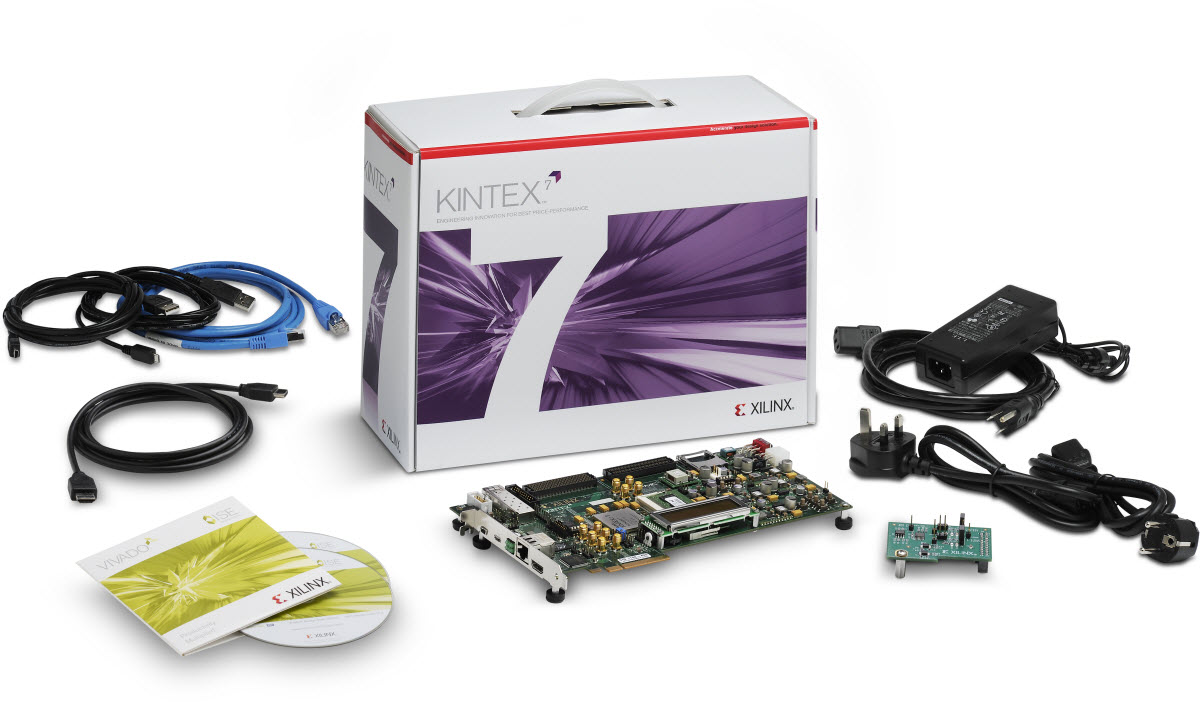
\includegraphics[width=0.7\textwidth]{fig/c3_desenvolvimento/intro/kintex-7_kc705}
\caption{Foto ilustrativa do kit de desenvolvimento Kintex-7 KC705 extraida do site da Xilinx.}
\label{fig:kc705}
\end{figure} 

\section{Material e Ferramentas Utilizados}
Foi utilizado para este projeto um computador com as especificações indicadas na tabela \ref{tab:specs}.
O conjunto de ferramentas utilizado foi o ISE Design Studio (versão 14.6).
Utilizou-se ainda o programa ActiveTcl (versão 8.6.1.0.297577) da ActiveState para a execução dos \textit{scripts} de compilação e o programa de código aberto Frhed (versão portátil 1.6r2) para a visualização de arquivos binários.

\begin{table}[h]
\centering
\begin{tabular}{| c | c |}
\hline
Componente & Especificação\\ \hline
Processador & Intel\textregistered Core i7-3630QM (4 núcleos a 2.4-3.4 GHz)\\\hline
Memória RAM & 12 GB\\\hline
Placa Gráfica Integrada & Intel\textregistered~HD Graphics 4000\\\hline
Placa Gráfica Principal & Nvidia\textregistered~GeForce GT 635M\\\hline
Sistema Operacional & Windows 7 Professional (64 bits)\\\hline
Portas USB & USBs 2.1 e 3.0\\\hline
\end{tabular}
\caption{Especificações do computador utilizado.}
\label{tab:specs}
\end{table}

Escolheu-se ainda utilizar o kit de desenvolvimento da Xilinx\textregistered{} chamado Kintex-7 KC705, mostrado na figura \ref{fig:kc705}.
O único critério utilizado foi a disponibilidade dos equipamentos no início do projeto e a capacidade do dispositivo de realizar a reconfiguração dinâmica parcial.
Este kit possui FPGA modelo XC7K325T-2FFG900C, leitor de cartão de memória, conector PCIe\textregistered{}, memória DDR3, visor de 7-segmentos e porta ethernet, dentre outros.

\ifx\compilewholereport\undefined
	\bibliographystyle{authordate1} 
	%\bibliography{bibliografia}
	\newsavebox\mytempbib\savebox\mytempbib{\parbox{\textwidth}{\bibliography{bibliografia}}}
	\listoftodos
	\end{document}
\fi

% *** Revisao Bibliografica ***
%TCIDATA{LaTeXparent=0,0,relatorio.tex}
\ifx\compilewholereport\undefined
	\documentclass[11pt,a4paper,oneside]{book}
	
	% Escolher um dos seguintes formatos:
	\usepackage{ft2unb} % segue padrão de fontes do Latex
	
	% Pacotes
	\usepackage{graphicx}
	\usepackage{amsfonts}
	\usepackage{amsmath}
	\usepackage{amssymb}
	\usepackage[thmmarks,amsmath]{ntheorem}
	\usepackage{boxedminipage}
	\usepackage{theorem}
	\usepackage{fancybox}
	\usepackage{fancyhdr}
	\usepackage{url}
	\usepackage{afterpage}
	\usepackage{color}
	\usepackage{colortbl}
	\usepackage{rotating}
	\usepackage{makeidx}
	\usepackage{indentfirst}
	\usepackage{bibentry}
	\usepackage{subcaption}
	\usepackage{todonotes}
	\presetkeys{todonotes}{inline}{}
	
	\begin{document}
	\frontmatter
	\listoftodos
	\mainmatter
	
	%%%%%%%%%%%%%%%%%%%%%%%%%%%%
	%%%%%%%% Apagar coisas acima
	%%%%%%%%%%%%%%%%%%%%%%%%%%%%
\fi
                      
\chapter{Revisão Bibliográfica}\label{CapRevisaoBibliografica}

% Resumo opcional. Comentar se não usar.
\resumodocapitulo{Este capítulo visa apresentar o estado-da-arte da reconfiguração dinâmica e da auto-reconfiguração e as ferramentas necessárias para sua realização.}

\section{Introdução}
Os temas reconfiguração dinâmica, parcial e autoreconfiguração 

\subsection{Classes de Reconfigura\c{c}\~ao}
Com a chegada de CPLDs e FPGAs, requisitos cada vez mais complexos foram sendo introduzidos ao projeto de sistemas digitais.
Tais requisitos for\c{c}aram as ferramentas de s\'i­ntese a suportar diferentes classes de reconfigura\c{c}\~ao.
Note que reconfigura\c{c}\~ao diz respeito, como dito anteriormente, a modifica\c{c}\~ao do comportamento, ou configura\c{c}\~ao, de um dispositivo reconfigur\'avel.

\subsubsection{Reconfigura\c{c}\~ao Total}
A reconfigura\c{c}\~ao total, herdada da tecnologia tradicional, compreende a mudan\c{c}a do comportamento de todo o dispositivo reconfigur\'avel, sem exce\c{c}\~ao de blocos l\'ogicos.
Tal reconfigura\c{c}\~ao \'e bastante dispendiosa, visto que maior parte das alterações realizadas são incrementais e dizem respeito \`a apenas uma pequena parte do dispositivo.
Apesar disto, todos os FPGAs d\~ao suporte a este tipo de reconfigura\c{c}\~ao.

\subsubsection{Reconfigura\c{c}\~ao Parcial}
A reconfigura\c{c}\~ao parcial, ao contr\'ario da reconfigura\c{c}\~ao total, diz respeito \`a programa\c{c}\~ao de apenas parte de um dispositivo reconfigur\'avel \cite{Hauck2007}.
Para tal, faz-se necess\'ario a divis\~ao do dispositivo nas chamadas parti\c{c}\~oes, cada uma com sua configura\c{c}\~ao individual.
Desta forma, mudan\c{c}as feitas em uma parti\c{c}\~ao n\~ao afetam as outras, acelerando o processo de s\'i­ntese e programa\c{c}\~ao.
Outro processo que \'e acelerado \'e o de roteamento, uma vez que o particionamento introduz limita\c{c}\~oes no mapeamento das fun\c{c}\~oes.
Nem todos os FPGAs d\~ao suporte a este tipo de reconfigura\c{c}\~ao, que pode ser realizado tanto de forma dinâmica (\ref{sss:dinamica}) quando estática (\ref{sss:estatica}).

\subsubsection{Reconfigura\c{c}\~ao Est\'atica}
\label{sss:estatica}
O termo reconfigura\c{c}\~ao est\'atica se refere a programa\c{c}\~ao de um dispositivo reconfigur\'avel enquanto ele n\~ao estiver executando.
No caso em que alguma programa\c{c}\~ao j\'a tenha sido transferida para ele e ele a esteja executando, esta \'e parada para que o dispositivo seja configurado novamente.
Por ser mais f\'acil de ser implementada e n\~ao necessita de circuitos adicionais, todos os FPGAs d\~ao suporte a este tipo de reconfigura\c{c}\~ao.

\subsubsection{Reconfigura\c{c}\~ao Din\^amica}
\label{sss:dinamica}
A reconfigura\c{c}\~ao din\^amica acontece frente \`a necessidade de reprograma\c{c}\~ao parcial do dispositivo sem que ele pare de funcionar.
As funcionalidades modificadas s\~ao interrompidas e substituidas sem afetar o funcionamento do todo.
Normalmente este processo, quando n\~ao associado a autorreconfigura\c{c}\~ao, \'e realizado atrav\'es de um circuito externo à FPGA, tal como um controlador, um microcontrolador, ou mesmo um computador, como apresentado na figura \ref{fig:rexterna}.
Quase todos os FPGAs modernos d\~ao suporte a esta tecnologia.

\begin{figure}[htp]
\centering
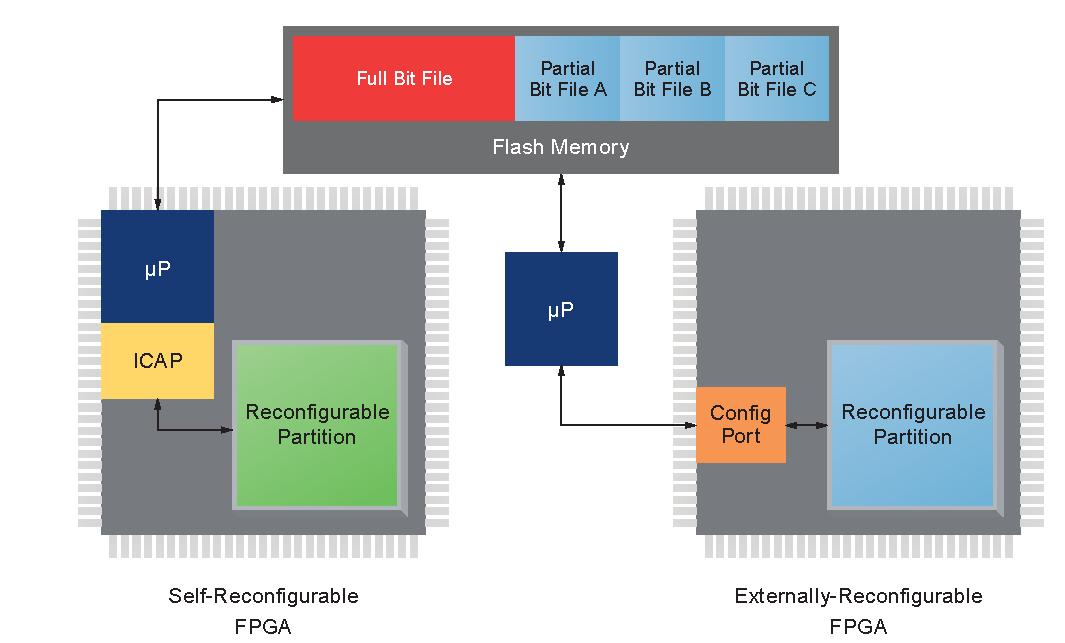
\includegraphics[width=0.8\textwidth]{fig/c1_introducao/reconf_externa.pdf}
\caption{Imagem ilustrativa para diferenciação entre autorreconfiguração e reconfiguração externa, extraido de \cite{wp374}.}
\label{fig:rexterna}
\end{figure}

É implicito o uso da reconfiguração parcial com a reconfiguração dinâmica, uma vez que faz pouco sentido reconfigurar todo o FPGA enquanto ela ainda está em execução.
Note que este tipo de reconfiguração em geral também necessita de uma parte permanentemente est\'atica, para interfacear com o circuito controlador.
Esta parti\c{c}\~ao est\'atica \'e respons\'avel pelo menos por controlar a comunica\c{c}\~ao com o circuito controlador.

Vale lembrar que a este tipo de reconfiguração, apesar de abrir muitas possibilidades, introduz uma necessidade de preocupação com \textit{overheads} de reconfiguração \cite{Hauck2007}.
Este \textit{overhead} é proporcional ao tamanho da partição que se deseja modificar e inversamente proporcional às velocidades das interfaces de reconfiguração.
Tal fator pode se tornar crucial na escolha entre o uso desta tecnologia ou alguma outra alternativa, possivelmente multiplexada.
Note que existem outros fatores que influenciam na opção por reconfiguração dinâmica, tais como preço, capacidade e potência, dentre outros, que não serão considerados aqui.

\subsubsection{Autorreconfigura\c{c}\~ao}
Modalidade de reconfigura\c{c}\~ao din\^amica parcial onde a reconfigura\c{c}\~ao do dispositivo \'e decidida por uma l\'ogica pertencente a ele mesmo.
Normalmente usa-se um microcontrolador ou uma m\'aquina de estados finitos para controlar a mudan\c{c}a de configura\c{c}\~oes.
Este tecnologia \'e nova e ainda representa uma forte \'area de pesquisa.
Por isso n\~ao s\~ao todos os FPGAs que d\~ao suporte a este tipo de reconfigura\c{c}\~ao.

Para que a autorreconfigura\c{c}\~ao aconte\c{c}a, os \textit{bitstreams}, resultado da sintetiza\c{c}\~ao, devem ser passados para uma mem\'oria acess\'i­vel ao FPGA durante a execu\c{c}\~ao do mesmo.
O circuito controlador identifica ent\~ao um padr\~ao que defina a necessidade de reconfigura\c{c}\~ao e transfere o \textit{bitstream} correspondente a esta nova necessidade para a parti\c{c}\~ao destino, que assim muda seu comportamento.
Note que para tal, as entradas e sa\'i­das das parti\c{c}\~oes tem que ser fixas, para que a mudan\c{c}a nas configura\c{c}\~oes das parti\c{c}\~oes n\~ao danifique o FPGA em si.

\todo{Apresentar o estado-da-arte}

\section{Ferramentas}
Diversas ferramentas foram utilizadas para a realização deste trabalho.
Dentre eles pode-se citar os programas da Xilinx, interpretadores da linguagem Python, Perl e Tcl, compiladores de \LaTeX e a ferramenta de controle de versão Git.
Abaixo segue uma pequena descrição sobre estas ferramentas mais críticas.

\subsection{Xilinx ISE Design Suite}
O \textit{ISE Design Suite} é um conjunto de ferramentas da Xilinx para o desenvolvimento de projetos de \textit{hardware}.
Estes programas estão apresentados a seguir.

\subsubsection{Xilinx ISE Design Tools}
O \textit{ISE Design Tools}, disponível para os sistemas Windows XP (32 e 64 bits), Windows 7 (32 e 64 bits), Windows Server 2008 (64 bits), Red Hat Enterprise 5 e 6 (32 e 64 bits) e SUSE Linux Enterprise 11 (32 e 64 bits) \cite{ug631}, controla todos os aspectos do fluxo de projeto \cite{ug695}.
Através do \textit{Project Navigator}, sua principal ferramenta, é possivel acessar todas as configurações e ferramentas de implementação de configurações.

\paragraph{\textit{Project Navigator}} O \textit{Project Navigator} é a principal ferramenta do \textit{ISE Design Tools}.
Através dela é possível criar projetos, incluir arquivos de descrição de \textit{hardware}, seja em VHDL, Verilog ou esquemáticos, construir componentes de propriedade intelectual, impor restrições e compilá-los, dentre outras coisas.

\paragraph{iMPACT}
\paragraph{\textit{Core Generator}}

\subsubsection{\textit{Embedded Development Kit}}
\paragraph{Xilinx Platform Studio}
\paragraph{Xilinx Software Development Kit}

\subsubsection{PlanAhead}
\subsubsection{ChipScope}
\subsubsection{System Generator}
\subsubsection{Ferramentas de Linha de Comando}
\paragraph{Xilinx Sinthesis Tool (XST)}


\section{Componentes}
\subsection{\textit{Intellectual Property}}
\todo{Clock}
\todo{Memória DDR3, MIG, MIS}
\subsection{Interfaces}
\todo{SelectMAP}
\todo{ICAP e ICAPE2}

\ifx\compilewholereport\undefined
	\bibliographystyle{authordate1} 
	%\bibliography{bibliografia}
	\newsavebox\mytempbib\savebox\mytempbib{\parbox{\textwidth}{\bibliography{bibliografia}}}

	\end{document}
\fi

\part{Desenvolvimento}
% *** Desenvolvimento ***
%TCIDATA{LaTeXparent=0,0,relatorio.tex}
\ifx\compilewholereport\undefined
	\documentclass[11pt,a4paper,oneside]{book}
	
	% Escolher um dos seguintes formatos:
	\usepackage{ft2unb} % segue padrão de fontes do Latex
	
	% Pacotes
	\usepackage{graphicx}
	\usepackage{amsfonts}
	\usepackage{amsmath}
	\usepackage{amssymb}
	\usepackage[thmmarks,amsmath]{ntheorem}
	\usepackage{boxedminipage}
	\usepackage{theorem}
	\usepackage{fancybox}
	\usepackage{fancyhdr}
	\usepackage{url}
	\usepackage{afterpage}
	\usepackage{xcolor}
	\usepackage{rotating}
	\usepackage{makeidx}
	\usepackage{indentfirst}
	\usepackage{subcaption}
	\usepackage{todonotes}
	\usepackage{listings}
	\presetkeys{todonotes}{inline}{}
	
	\begin{document}
	\frontmatter
	\listoftodos
	\tableofcontents
	\mainmatter
	
	%%%%%%%%%%%%%%%%%%%%%%%%%%%%
	%%%%%%%% Apagar coisas acima
	%%%%%%%%%%%%%%%%%%%%%%%%%%%%
	\newcommand\qt[1]{\lq\lq{}#1\rq\rq{}}
	\newcommand\qti[1]{\lq\lq{}\textit{#1}\rq\rq{}}
\fi

\lstdefinestyle{customVHDL}{
	  belowcaptionskip=1\baselineskip,
	  breaklines=true,
	  frame=l,
	  xleftmargin=\parindent,
	  language=VHDL,
	  showstringspaces=false,
	  basicstyle=\footnotesize\ttfamily,
	  keywordstyle=\itshape\color{blue!40!black},
	  commentstyle=\itshape\color{blue!40!black},
	  identifierstyle=\itshape\color{blue!40!black},
	  stringstyle=\itshape\color{blue!40!black},
}
                      
\chapter{Desenvolvimento}\label{CapDesenvolvimento}

\resumodocapitulo{Este capítulo trata da concepção dos experimentos realizados. Nele serão descritos com detalhes cada um dos experimentos, ficando a parte de análise reservada ao capítulo \ref{CapExperimentos}.}

\section{Introdu\c{c}\~{a}o}
%\vspace{0.8cm}
Devido ao caráter experimental e exploratório do objetivo proposto na seção \ref{sec:projeto}, decidiu-se dividir o projeto em vários experimentos menores.
Desta forma, além de garantir algum material mesmo que tudo dê errado, consegue-se simplificar o processo de pesquisa e desenvolvimento através dos pequenos passos e análises frequentes.

Como o objetivo final do projeto é a familiarização com as ferramentas e processos envolvidos na autoreconfiguração, decidiu-se começar estudando os elementos necessários para se realizar a reconfiguração dinâmica.
O passo seguinte mais lógico é o de estudar como funciona as memórias dos sistema e de que jeito elas seriam melhor utilizadas.
O último passo seria entender como funciona a autoreconfiguração em baixo nível, ou seja, como os dados devem ser entregues aos devidos componentes para que ela aconteça.
Para cada um destes experimentos foi proposto um teste que validasse o completo entendimento do mesmo.

\begin{figure}[h]
\centering
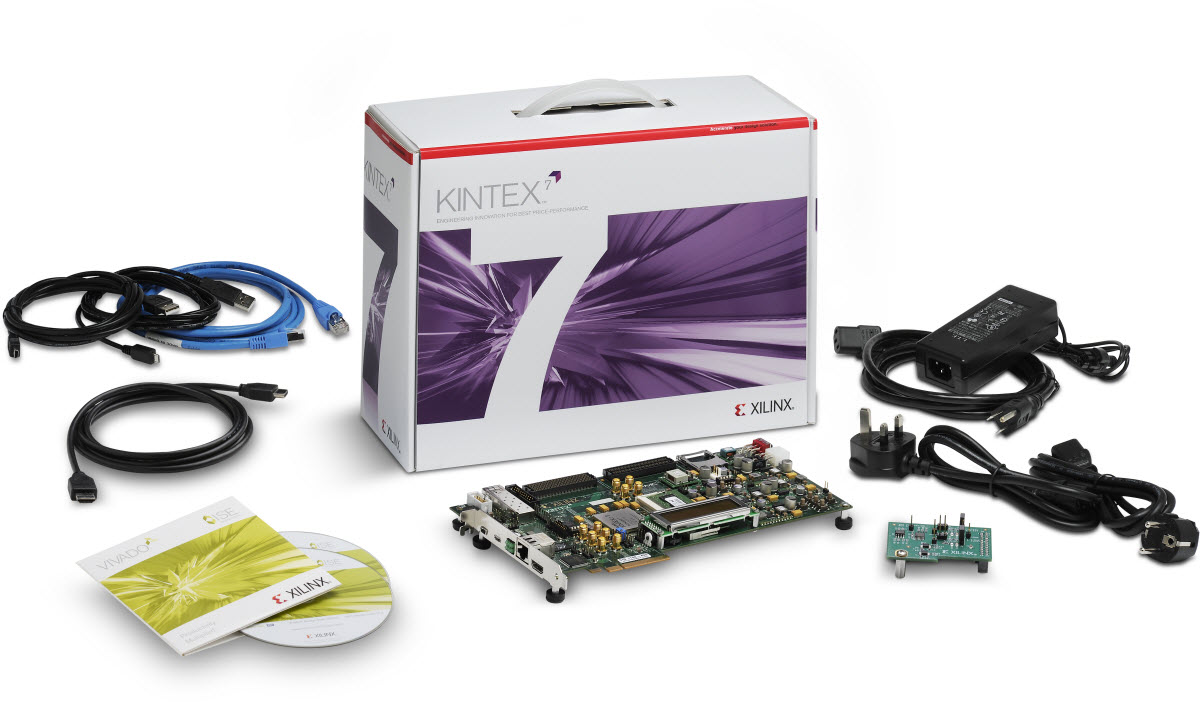
\includegraphics[width=0.7\textwidth]{fig/c3_desenvolvimento/intro/kintex-7_kc705}
\caption{Foto ilustrativa do kit de desenvolvimento Kintex-7 KC705 extraida do site da Xilinx.}
\label{fig:kc705}
\end{figure}

Para o desenvolvimento desse projeto, escolheu-se utilizar o kit de desenvolvimento da Xilinx\textregistered{} chamado Kintex-7 KC705.
O único critério utilizado foi a disponibilidade dos equipamentos no início do projeto e a capacidade do dispositivo de realizar a reconfiguração parcial dinâmica.
Este kit possui FPGA modelo XC7K325T-2FFG900C, leitor de cartão de memória, conector PCIe\textregistered{}, memória DDR3, visor de 7-segmentos e porta ethernet, dentre outros.

Escolheu-se ainda, de forma arbitrária, o uso da linguagem VHDL para a descrição de \textit{hardware} ao invés da Verilog.

\section{Experimento 1 - Reconfiguração Dinâmica}
De forma a dar validade a todo o projeto, foi preciso desenvolver um experimento para se entender o processo de desenvolvimento de sistemas reconfiguráveis dinamicamente e algumas peculiaridades do kit de desenvolvimento.

\subsection{Fluxo de Ferramentas}
A primeira coisa que se destaca no desenvolvimento de dispositivos dinamicamente reconfiguráveis é a diferença no fluxo de ferramentas, também conhecido como \textit{software tools flow}, em relação ao fluxo tradicional \cite{ug743}.
Esta diferença é motivada pela necessidade de construção de diversos \textit{bitfiles} parciais.
Como pode-se ver da figura \ref{fig:ex1:softwareflow}, o fluxo tradicional requer apenas o uso do programa ISE, e opcionalmente do XPS e do SDK, para a construção de um projeto de \textit{hardware} e o iMPACT para a programação da FPGA.
No fluxo para reconfiguração dinâmica mostrado na figura \ref{fig:ex1:prsoftwareflow}, além das ferramentas do fluxo tradicional, faz-se necessário o uso da ferramenta XST para a síntese do \textit{netlist} e do PlanAhead para a definição de partições e configurações.
Note que estes fluxos não apresentam as únicas opções de fluxo de ferramentas, mas as que foram utilizadas neste projeto.

\begin{figure}[h]
	\centering
       	\begin{subfigure}[b]{\textwidth}
       		\centering
		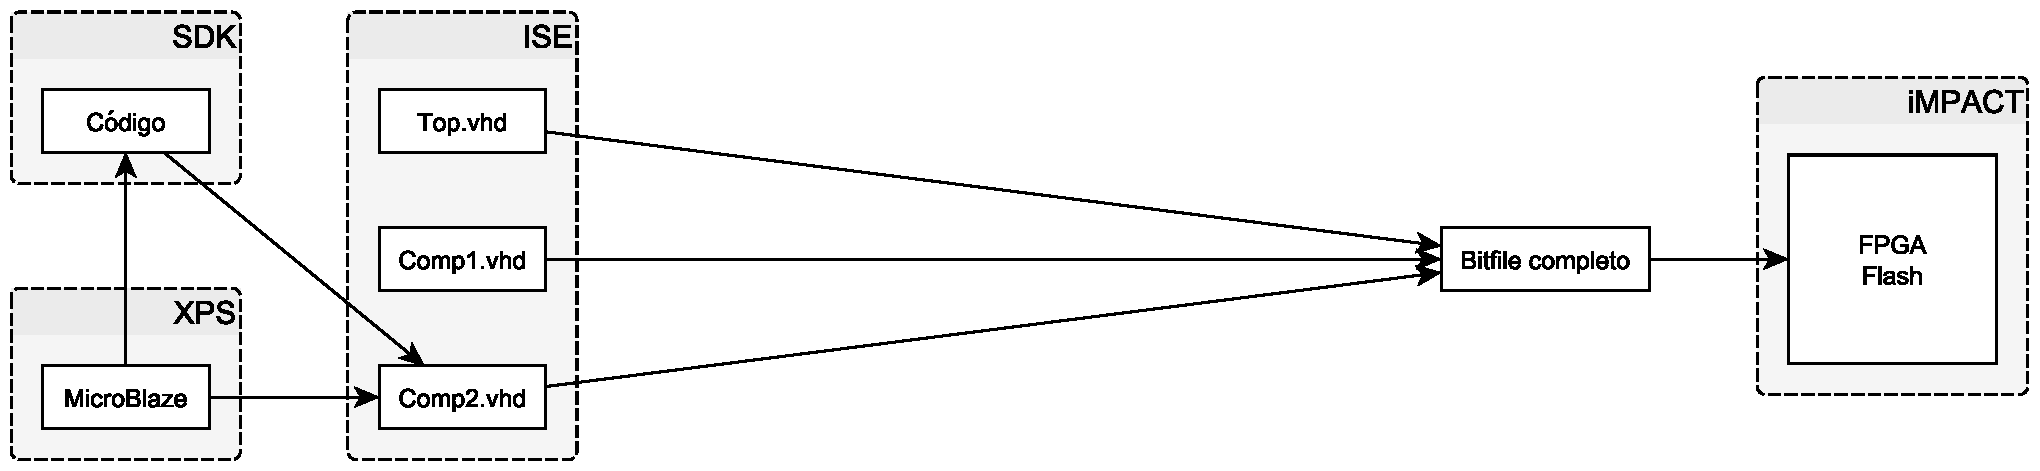
\includegraphics[height=100px]{fig/c3_desenvolvimento/ex1/softwareflow.pdf}
		\caption{Foto ilustrativa do fluxo de ferramentas tradicional. Note que o uso do microcontrolador MicroBlaze é opcional, tornando os primeiros blocos, SDK e XPS, também opcionais.}
		\label{fig:ex1:softwareflow}
	\end{subfigure}\\
	\begin{subfigure}[b]{\textwidth}
		\centering
		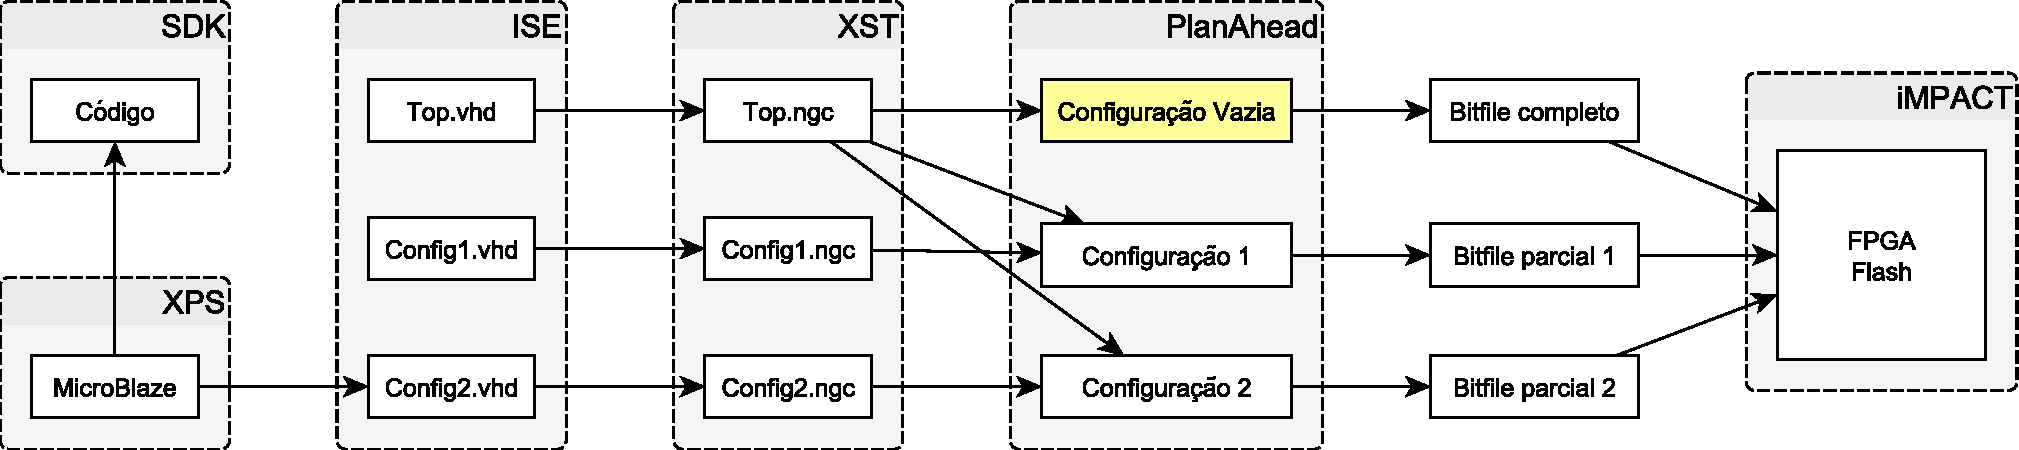
\includegraphics[height=100px]{fig/c3_desenvolvimento/ex1/prsoftwareflow.pdf}
		\caption{Foto ilustrativa do fluxo de ferramentas para a reconfiguração dinâmica. Assim como no caso tradicional, o uso do SDK e do XPS são opcionais. Note que o bloco em amarelo indica a configuração padrão, que será programada inicialmente. A escolha da configuração padrão é arbitrária.}
		\label{fig:ex1:prsoftwareflow}
	\end{subfigure}
	\caption{Comparação dos fluxos de ferramentas. Note que estes fluxos não apresentam as únicas opções de fluxo de ferramentas, mas as que foram utilizadas neste projeto.}
	\label{fig:ex1:softwareflow:comparacao}
\end{figure}

Reconfiguração parcial pede uma síntese utilizando o método \qt{de baixo para cima} (\textit{bottom-up}), mas uma implementação \qt{de cima para baixo} (\textit{top-down}) \cite{ug743}, ou seja, a implementação acontece construindo primeiro a interface com o sistema e depois os componentes auxiliares, mas a síntese precisa ser realizada no sentido oposto.
Esta implementação é equivalente a se construir diversos projetos tradicionais com alguma lógica em comum, onde a síntese deve garantir que esta lógica em comum seja implementada da mesma forma para as diferentes configurações \cite{ug702}.

\subsection{Peculiaridades}
O kit de desenvolvimento utilizada apresenta algumas peculiaridades com relação aos kits comuns.
A seguir serão apresentadas algumas destas peculiaridades.

\subsubsection{Relógios}
Diferentemente das FPGAs comuns, a que está presente neste kit contém um relógio diferencial, ou seja, dois sinais compoem tal relógio.
A razão para tal é a presença de circuitos sensíveis a interferência, tais como \textit{transceivers}, que são muito menores em sinais diferenciais.
O kit disponibiliza duas opções de relógio: o SYSCLK e o USER\_CLOCK.
O primeiro possui uma frequência fixa de oscilação de 200 MHz.
O segundo possui uma frequência original de 156,250 MHz, mas pode ser programado através de uma interface I$^2$C para ter frequências entre 10 MHz e 810 MHz.
Por motivos de simplicidade, utilizou-se o SYSCLK.
Para poder se trabalhar com o sinal diferencial, construiu-se, utilizando as ferramentas do ISE, um componente para tratamento do sinal de relógio.
Este componente recebe o sinal diferencial, reduz sua frequência para 20 MHz, que corresponde ao menor valor suportado pelas PLLs da placa, e emite um sinal convencional.

\subsection{Teste}
Para se entender mais a fundo o fluxo de projeto, nada melhor que construir um projeto.
Para isso, implementou-se o sistema esquematizado na figura \ref{fig:ex1:componentes}.
Este sistema contém o \qt{Top} para interfaceamento com a FPGA, o \qt{Clocks} para tratamento do sinal de relógio, a \qt{Static}, que possui um lógica estática para demonstrar que a reconfiguração de uma partição não interfere com outra, e a \qt{Dynamic}, que possui a lógica a ser alterada dinâmicamente.

\begin{figure}[h]
\centering
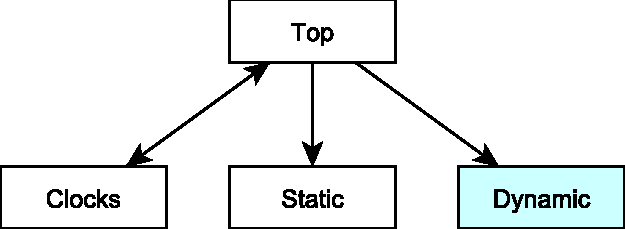
\includegraphics[width=0.5\textwidth]{fig/c3_desenvolvimento/ex1/componentes.pdf}
\caption{Foto ilustrativa do sistema desenvolvido para o teste de validação do experimento 1. Ele é composto por uma parte estática e uma parte dinâmica. O elementos em branco são estáticos e os em azul são dinâmicos.}
\label{fig:ex1:componentes}
\end{figure}

\paragraph{Estrutura de Pastas}
A questão da organização do projeto em pastas bem específicas é sempre bem mencionado na literatura \cite{ug702, ug743, ug744}.
Os manuais recomendam a seguinte estrutura de pastas.
\begin{lstlisting}
Projeto/
  Source/           //codigos-fonte organizados segundo particao
  Implementation/   //contem pastas para cada config. dinamica gerada
  Synth/            //contem pastas com os arquivos .xst e .prj
  Tools/            //ferramentas para automacao da sintese
  PlanAhead/        //pasta para o projeto do PlanAhead
\end{lstlisting}
Esta estrutura de pastas foi obedecida por ajudar a manter o ambiente de desenvolvimento limpo.

\subsubsection{Comportamento}
Como explicado anteriormente, o projeto de um sistema parcialmente reconfigurável pode ser visto como vários projetos completos com partes em comum.
Seguindo essa lógica, dois projetos com comportamentos diferentes foram construídos usando como base a figura \ref{fig:ex1:componentes}.
O comportamento individual de cada módulo ou componente será descrito a seguir.
Este passo está ilustrado no fluxo de ferramentas da figura \ref{fig:ex1:prsoftwareflow} como ISE.

O componente \qt{Static} possui uma entrada para um relógio pulsando a 2 Hz e uma saída para um LED.
Seu comportamento apenas faz com que o LED pisque a uma frequência de 2 Hz, o que permite observar seu funcionamento durante a reconfiguração do componente \qt{Dynamic}.

O componente \qt{Dynamic} possui dois comportamentos distintos.
O primeiro deles é o de um simples contador crescente de 4 bits.
O segundo é uma máquina de estados que alterna os 4 bits de saída entre "1100" e "0011" a cada pulso de relógio.
Este componente possui uma entrada para um relógio pulsando a 1 Hz e uma palavra de 4 bits de saída.
A frequência de operação deste componente foi escolhida para ser a metade da frequência da \qt{Static} para poder ser visualmente comprovado que \qt{Static} não para de funcionar quando \qt{Dynamic} está sendo reconfigurado.

O componente \qt{Clocks} recebe os sinais diferenciais de relógio e o transformam em um sinal comum.
O bloco lógico utilizado para isso foi construído usando ferramentas presentes no ISE.
Uma vez que a ferramenta permitia a construção de um relógio com divisor de frequência, a frequência do relógio da placa, que nesse caso é de 200 MHz, foi reduzida para 20 MHz.

O módulo \qt{Top} instancia os componentes descritos acima e faz a interface dos mesmos com a FPGA.
O componente dinâmico precisa de uma declaração de protótipo para ser instanciado corretamente.
Utilizou-se o código abaixo para esta finalidade.
\begin{lstlisting}[style=customVHDL]
component dynamic
    port ( clk  : in  std_logic;
           leds : out std_logic_vector (3 downto 0));
end component;
\end{lstlisting}
O módulo \qt{Top} possui também um divisor de frequência para reduzir a frequência devolvida por \qt{Clocks} para 1 e 2 Hz.

\subsubsection{Síntese}
Com o comportamento do projeto definido, o próximo passo segundo o fluxo de ferramentas é a síntese.
Este passo é necessário uma vez que o próximo passo, referente ao PlanAhead, não aceita como entrada códigos-fonte.
Os códigos-fonte precisam passar por uma etapa de síntese separada para poderem ser importados no PlanAhead.
Este passo está ilustrado no fluxo de ferramentas da figura \ref{fig:ex1:prsoftwareflow} como XST.

O comando XST recebe tipicamente um \textit{script} contendo o endereço dos códigos-fonte, o nome do arquivo de saída, o tipo do arquivo de saida, o modelo da FPGA utilizada e uma indicação do código-fonte principal.
O comando para iniciar o processo é o seguinte.
\begin{lstlisting}[style=customVHDL]
xst.exe -ifn Top.xst
\end{lstlisting}
O arquivo \qt{Top.xst} contém os seguintes comandos.
\begin{lstlisting}[style=customVHDL]
run
-ifn Top.prj
-ofn Top
-ofmt NGC
-p xc7k325t-2-ffg900
-top top
\end{lstlisting}
O arquivo \qt{Top.prj} contém os endereços dos arquivos, conforme a seguir.
\begin{lstlisting}[style=customVHDL]
vhdl work "../../Sources/static/top.vhd"
vhdl work "../../Sources/static/static.vhd"
vhdl work "../../Sources/static/clocks.vhd"
\end{lstlisting}\

Note que estes comandos e arquivos indicados acima são para síntese dos componentes estáticos.
Uma vez que não existe nenhuma restrição especial para tais componentes, eles podem ser síntetizados para um único arquivo de saída.
O mesmo não pode ser dito para os elementos dinâmicos.
Cada componente dinâmico precisa ser sintetizado em separado para depois ser incluído no projeto através do PlanAhead.

A síntese de componentes dinâmicos precisa ser realizada com um \textit{script} \qt{.xst} ligeiramente diferente.
Como mostrado a seguir, faz-se necessária a inclusão do argumento \qt{-iobuf NO}, que desabilita a inserção de componentes de Entrada/Saída \cite{ug743, ug748}.
\begin{lstlisting}[style=customVHDL]
run
-ifn DynFSM.prj
-ofn DynFSM
-ofmt NGC
-p xc7k325t-2-ffg900
-top dynamic
-iobuf NO
\end{lstlisting}
Note que o arquivo \qt{DynFSM.prj} contém informações sobre o cógigo-fonte do componente dinâmico, como mostrado a seguir.
\begin{lstlisting}[style=customVHDL]
vhdl work "../../Sources/dynamic_fsm/dynamic.vhd"
\end{lstlisting}

Existe também a possibilidade de construção de um \textit{script} para a síntese automática de todos os arquivos.
Utilizou-se aqui uma adaptação do arquivo em linguagem TCL usado pela Xilinx em seus manuais \cite{ug702, ug743, ug744}.
A única coisa que se faz neste \textit{script} é a construção dinâmica dos comandos com base em listas de arquivos pré-informados.

\subsubsection{PlanAhead}
Com os arquivos síntetisados, pode-se começar a etapa referente ao PlanAhead.
Nela, importaremos os arquivos da etapa anterior, criaremos a partição reconfigurável, mapearemos esta partição no dispositivo, criaremos configurações alternativas, promoremos tais configurações e geraremos os \textit{bitfiles} para a programação do dispositivo.
Note que é preciso uma licença do ISE que permita o uso do PlanAhead e de reconfiguração parcial.

O primeiro passo necessário no PlanAhead é a criação do projeto.
Para isso, após a abertura do programa, clica-se no ícone superior esquerdo mostrado na figura \ref{fig:ex1:planahead}, onde se lê \qt{Create New Project}.
Na janela que aparece, indicamos o nome do projeto e seu caminho, lembrando que foi criada uma pasta anteriormente especificamente para conter este projeto.
Indicamos também que o projeto é do tipo \qt{\textit{Post-synthesis Project}} e que desejamos habilitar a reconfiguração parcial, indicamos quais \textit{netlists} compõe o comportamento do projeto e qual corresponde ao arquivo principal, qual é o arquivo de restrições (\textit{constrains}) e qual é o modelo da FPGA.

\begin{figure}[h]
\centering
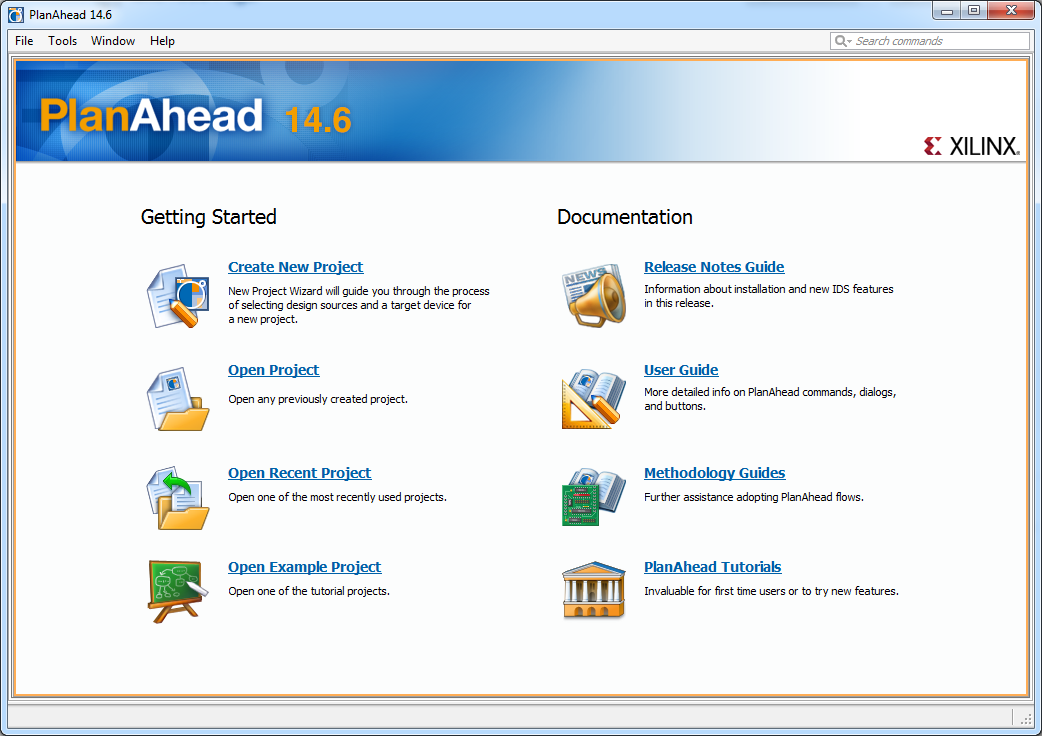
\includegraphics[width=0.9\textwidth]{fig/c3_desenvolvimento/ex1/PlanAhead}
\caption{Imagem do PlanAhead logo que aberto.}
\label{fig:ex1:planahead}
\end{figure}

Após a criação do projeto, carregam-se os arquivos sintetizados abrindo \qt{\textit{Open Synthesized Design}}, mostrado na figura \ref{fig:ex1:planahead_open_synthesized_design}.
Duas janelas de avisos aparecem, informando que existe uma partição não implementada e aviso sobre alguns pinos.

\begin{figure}[h]
\centering
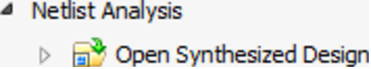
\includegraphics[width=173px]{fig/c3_desenvolvimento/ex1/planahead_open_synthesized_design}
\caption{Imagem do menu \qt{\textit{Open Synthesized Design}}.}
\label{fig:ex1:planahead_open_synthesized_design}
\end{figure}


Pode-se agora definir a partição que armazenará o componente dinâmico.
Isso é feito através do painel \qt{\textit{Netlist}}, selecionando a opção \qt{\textit{Set Partition}} do menu que aparece ao se clicar em \qt{dynamic\_i} com o botão direito.
Na janela que aparece, selecionamos a opção referente à partição reconfigurável, nomeamos o módulo reconfigurável de acordo com o componente que será carregado e indicamos o arquivo que corresponde ao arquivo sintetizado do componente reconfigurável.
Não é necessário informar restrições, visto que o componente, seguindo recomendações, não acessa os pinos de entrada e saída diretamente.
Note ainda que é recomendado que o primeiro módulo a ser incluído seja o mais complexo e sucetível a falhas, permitindo que erros e falhas na definição da região a seguir sejam identificados mais cedo.

Precisa-se definir também uma região para a partição recém definida.
Isto pode ser feito pelo mesmo painel \qt{\textit{Netlist}}, selecionando a opção \qt{\textit{Set Pblock Size}} do menu que aparece ao se clicar em \qt{dynamic\_i} com o botão direito.
Nesse momento, precisa-se selecionar na aba \qt{\textit{Device}} uma região do dispositivo que contenha uma quantidade de recursos maior que a requerida pelo projeto.
Note que o processo de escolha dessa região não é bem definido, o que abre espaço para diversos erros de alocação.
Para testar se a região foi bem alocada, abre-se a aba \qt{\textit{Design Runs}} do painel inferior, clica-se com o botão direito na única configuração disponível no momento e seleciona-se \qt{\textit{Run Launch}}.
Este processo pode demorar.
Em tentativas subsequentes, seleciona-se a opção de recomeçar todo o processo do zero, evitando erros gerados nos estágios iniciais.
Uma região possível, que foi utilizada nesse projeto, foi a que contém as células (\textit{slice}) de X80Y244 a X139Y205.
Os nomes das células ficam visíveis através da ampliação do dispositivo.

Uma vez terminado o \qt{\textit{Design Run}}, adiciona-se duas novas possibilidades de módulos reconfiguráveis para esta partição: um com comportamento definido e outro vazia.
Para isso, clica-se em \qt{\textit{Synthesized Design}} novamente e seleciona-se a opção \qt{\textit{Add reconfigurable module}} do menu que aparece ao se clicar em \qt{dynamic\_i} no painel \qt{\textit{Netlist}} com o botão direito.
O processo é o mesmo da definição da partição, sendo a única mudança na seleção do arquivo sintetizado e do nome do módulo.
Um módulo vazio pode ser criado usando esta mesma opção, mas selecionando a opção que indica a inclusão de uma \textit{blackbox} sem o uso de uma \textit{netlist}.

Com as possibilidades de módulos reconfiguráveis definidas, pode-se construir várias configurações.
Isso é feito através do clique com botão direito na \qt{\textit{Design Runs}} do painel inferior e selecionando-se a opção \qt{\textit{Create Runs...}}.
A janela que abre possui um painel chamado \qt{\textit{Create Implementation Runs}}.
Nesse painel, na coluna \qt{\textit{Partition Action}}, define-se, na coluna \qt{\textit{Module Variant}} da nova janela que aparece, o módulo desejado.
Voltando para a primeira janela, clica-se em \qt{\textit{More}} para adicionar a última configuração desejada.
Em seguida, as duas novas configurações serão criadas através de \qt{\textit{Design Runs}}.
É necessário promover neste momento a primeira configuração implementada.
O processo de promoção será comentado a seguir.
Note que os avisos que aparecerem podem ser ignorados.

Ao final dos \qt{\textit{Design Runs}}, recomenda-se fazer a verificação das configurações através do painel \qt{\textit{Configurations}}.
Clicando-se com o botão direito, encontra-se a opção \qt{\textit{Verify Configuration...}}, que faz com que uma janela seja aberta.
Selecionado-se todos os itens e clicando em \qt{\textit{OK}}, a verificação se inicia.
Nenhum erro deve ser encontrado.

Devemos agora promover as configurações.
No menu de quando se clica com o botão direito sobre as configurações já existentes do painel \qt{\textit{Configurations}}, seleciona-se \qt{\textit{Promote Configuration...}}.
A promoção de uma configuração é o equivalente a sua exportação \cite{ug748}.
Promover a primeira configuração antes de implementar novas contribui para manter a parte estática, compartilhada, igual em todas as configurações, uma vez que elas não mais são sintetizadas e sim importadas.

O último passo necessário para a criação dos \textit{bitfiles} é o \qt{\textit{Generate Bitstream}}, localizado no menu a esquerda.
Este passo recebe o resultado das sínteses e implementações e transforma-os em \textit{bitfiles}.
Esta etapa precisa ser realizada com cada uma das configurações realizadas, ou alguma delas não terá seus \textit{bitfiles} gerados.
Tais \textit{bitfiles} podem ser encontrados na pasta do projeto, dentro das pastas com nome de cada configuração que ficam dentro de da pasta *.runs.
Existem dois arquivos \textit{bitfile} dentro de cada pasta, um maior, que contém a configuração completa, e outro menor que possui a configuração parcial.

\subsubsection{iMPACT}
Com os \textit{bitfiles} em mãos, usa-se-os para programar a FPGA através auxilio da ferramenta iMPACT. 
A primeira coisa a se fazer após abrir o programa é permitir que o sistema automaticamente crie um projeto.
Na janela que se abre, escolhe-se a opção \qt{\textit{Automatically connect to a cable and identify Boundary-Scan chain}} do item \qt{\textit{Configure devices using Boundary-Scan (JTAG)}}.
Quando pergunta-se se deseja-se atribuir uma nova configuração, pode-se clicar que sim e escolher um arquivo binário completo gerado na etapa anterior.
Normalmente escolhe-se a configuração vazia como configuração inicial para poupar energia.

Quando a configuração for completamente transmitida e implementada, observa-se que um LED está piscando com uma frequência de 2 Hz e todos os outros (acionados) estão acesos.
Isto acontece uma vez que o sitema atribui sinal ativo para os elementos desconectados.

Para realizar a reconfiguração parcial dinâmica, clica-se com o botão direito no símbolo do dispositivo que aparece no iMPACT e seleciona-se a opção \qt{\textit{Assign New Configuration File...}}.
Procura-se então pelos arquivos binários parciais localizados na pasta \textit{PlanAhead > PlanAhead.runs >} \qt{nome da configuração}.
Este arquivo possui \qt{partial} em seu nome, o que o diferencia do arquivo binário completo.
Note que utilizar os arquivos binários completos não gera erro, mas constitui reconfiguração total, não parcial.
Após a seleção da configuração desejada, o último passo necessário é a programação, que pode ser realizada clicando-se com o botão direito no dispositivo e selecionando-se a opção \qt{\textit{Program}}.

\subsection{Possíveis Erros}
\paragraph{Erros no código-fonte} Este é um dos erros mais comuns.
A melhor forma de previní-lo é através da construção dos diversos comportamentos/configurações individuais utilizando o ISE.
Para acelerar o processo, realiza-se apenas a síntese.

\paragraph{Erros na alocação de partições}
Um erro bastante comum que aparece no PlanAhead é o de erro de alocação\footnote{\textit{AR\# 53290: Partial Reconfiguration - 7 series device layout of tiles (CLB, DSP, BRAM, INT) and a shared clocking structure of vertical clock spines between interconnect (routing) tiles}. Disponível em \url{http://www.xilinx.com/support/answers/53290.htm}}.
Existem duas possíveis formas de corrigí-lo: modificando-se o arquivo de restrições UCF ou alterando a região da partição.
A primeira forma, que ajuda a garantir que todos os recursos reconfiguráveis estão incluidas na região da partição, é a inclusão de \qt{INCLUSIVE=ROUTE} na linha que contém \qt{INST "dynamic\_i" AREA\_GROUP = "pblock\_dynamic\_i"}.
A segunda forma é simplemente mudando a posição da região da partição para a direita, para a esquerda ou sua largura, de acordo com a mensagem de erro retornada.
Esta método não é determinístico e pode ser necessárias várias tentativas antes de se conseguir uma partição mapeável. 

\paragraph{Esquecer de promover a partição}
A promoção da primeira configuração antes de se implementar as seguintes contribui para a implementação de configurações compatíveis.
Esquecer de promover esta partição pode fazer com que erros sejam gerados na etapa de verificação das partições.

\paragraph{O PlanAhead pode travar enquanto implementando uma configuração}
Apesar de mais raro, o PlanAhead pode travar quando implementando uma configuração.
A melhor solução é o reinício do computador, visto que o programa bloqueia alguns arquivos durante a implementação e não os desbloqueia quando fechado forçadamente.

\paragraph{Erros na detecção da placa}
Note que algum programa aberto pode interferir com a varredura realizada pelo iMPACT, fazendo-a falhar.
Para prevenir este erro, deve-se fechar o XPS, o SDK e qualquer outro programa que possa se utilizar das interfaces USB.
Note ainda que a placa deve estar ligada para poder ser detectada.

\subsection{Conclusão}
O processo de desenvolvimento de partições reconfiguráveis e sua programação foi explorado com sucesso.
Observou-se os pontos críticos do desenvolvimento e o fluxo mais adequado para a construção deste tipo de projeto.

\section{Experimento 2 - Teste de Memórias}
Seguindo o raciocínio apresentado no início do capítulo, o próximo passo natural no desenvolvimento deste projeto é o entendimento do funcionamento das memórias.
Esta etapa abre caminho para que se armazene os \textit{bitfiles} de configurações parciais em uma memória embarcada, removendo a necessidade do computador para tal.

\subsection{Tipos de Mémoria}

No kit utilizado existem vários tipos de memórias que poderiam ser usados, cada um com suas peculiaridades \cite{ug810}.
Este experimento foi dedicado à compreenção do funcionamento dos diversos tipos de memórias e à escolha da solução mais adequada.

\subsubsection{Memória \textit{Block RAM}}
A memória do tipo \textit{Block RAM} é construída usando-se os blocos de memória RAM restantes da FPGA.
Esta memória consegue alcançar velocidades de leitura na ordem de várias centenas de hertz, mas possui uma capacidade de armazenamento bem reduzida, de apenas 445 blocos de 36 Kb para este kit, totalizando um máximo de aproximadamente 2 MB \cite{ug473, wp377}.
Note que a configuração total da FPGA necessita de aproximadamente 11 MB, ou exatamente 91.548.896 bits, para sua programação total \cite{ug470}.
Pode-se programá-la através do iMPACT, dentre outras formas \footnote{\textit{Memory Initialization Methods}, escrito por Jim Wu em 31 de dezembro de 2011. Dísponível em \url{http://myfpgablog.blogspot.com.br/2011/12/memory-initialization-methods.html}}.

\subsubsection{Memória \textit{Distributed RAM}}
A memória \textit{Distributed RAM} é construida utilizando-se das LUTs disponíveis nas célula lógicas \cite{ug473, wp377}.
Também são muito rápidas, apesar de síncronas, e também possuem pouca capacidade de armazenamento.
Pode-se programá-la através do iMPACT, dentre outras formas.

\subsubsection{Memória \textit{Linear BPI Flash}}
A memória \textit{Linear BPI Flash} disponibiliza 128 Mb de memória não-volátil \cite{ug810}, acessadas em palavras de 16 bits.
Apesar disso, sua velocidade de leitura máxima é de 33 MHz.
Convertendo tal velocidade para a leitura de 32 bits, tem-se uma velocidade de leitura de aproximadamente 16 MHz.
Pode-se programá-la através do iMPACT.

\subsubsection{Memória \textit{SPI Flash}}
A memória SPI Flash é diferente na sua forma de acesso, que acontece através da interface SPI.
Esta memória fornece 128 Mb de memória não volátil \cite{ug810}.
Ela aceita três modos de operação, x1, x2 e x4, que corresponde a largura da palavra lida/escrita a cada pulso de relógio \cite{N25Q128}.
A frequência de operação é de no máximo 50 MHz \cite{xapp586}.
Pode-se programá-la através do iMPACT.

\subsubsection{Cartão de Memória SD}
O cartão de memória SD dá acesso a uma memória não-volátil de tamanho arbitrário.
Esta interface permite o uso de cartões de alto desempenho, lendo palavras de 4 bits a frequências de até 50 MHz \cite{ug810}.
A limitação desta interface é a dificuldade de leitura e escrita devido ao sistema de arquivos inerente ao cartão.
Note que também não existe a possibilidade de programação do cartão através do iMPACT, o que resolveria o problema do sistema de arquivos.

\paragraph{\textit{CompactFlash} e o \textit{System ACE}}
\textit{SystemAce} é um sistema que permite a programação de FPGAs e memórias voláteis a partir de um cartão \textit{CompactFlash} \cite{ds080, ds583}.
Este é bem robusto e popular em séries que possuem um leitor deste tipo de cartão.

\subsubsection{Memória DDR3}
A memória DDR3 é uma memória volátil com 1 GB de capacidade de armazenamento e possui uma frequência de operação da ordem dos 800 MHz \cite{MT8JTF12864HZ}.
Só pode ser programada apenas em tempo de execução, fazendo-se necessário o uso de um \textit{bootloader}.

\subsection{Teste}
Notou-se no primeiro experimento que os \textit{bitfiles} parciais gerados possuem 645 KB, totalizando 1935 KB, ou 1,89 MB.
Com isso o uso das memórias que se utilizam de recursos internos da FPGA fica comprometido.
Caso se escolha esta opção, apenas os \textit{bitfiles} parciais poderiam ser armazenados, necessitando da ajuda do computador para a programação inicial.
Este típo de memória é mais útil como memória de dados e de programa em microcontroladores embarcados na FPGA, devido a sua altíssima velocidade de acesso e capacidade de acesso de vários canais em paralelo.

Observa-se que a interface de reprogramação dinâmica, ICAPE2, opera a uma frequência de até 100 MHz e pode receber palavras de até 32 bits, ou seja, 3200 Mb/s.
Por causa disso, todas as interfaces não-voláteis apresentadas acima acabariam por ser o gargalo do tempo da programação.
Uma solução é a implementação de um sistema que carregue as informações de uma memória não-volátil, tanto a Linear Flash quanto a SPI Flash seriam suficientes, para a memória DDR3 em um momento inicial, e depois permita que a memória DDR3 seja acessada para a reconfiguração dinâmica.
A forma mais fácil de implementar tal funcionalidade é através do uso de um microcontrolador MicroBlaze funcionando como \textit{bootloader}.

Antes de implementar o \textit{bootloader}, precisamos entender como funcionam as memórias do escolhidas.
Este teste, então, tem por objetivo entender o fluxo de projeto para o uso do MicroBlaze, o funcionamento deste microcontrolador e as formas corretas de se acessar as memórias do sistema.

\subsubsection{Fluxo de Projeto}
O procedimento para a construção de um projeto com MicroBlaze segue o fluxo descrito na figura \ref{fig:ex1:softwareflow}, no que diz respeito ao XPS e ao SDK.
A figura \ref{fig:ex2:softwareflow} apresenta o fluxo de ferramentas para este caso específico.
Em outras palavras, o fluxo espera que primeiro se desenvolva o microprocessador com todos os seus periféricos para depois se desenvolver o programa que será embarcado.
Tanto o programa quando o processador gerarão arquivos binários que serão carregados pelo iMPACT através do SDK.

\begin{figure}[htp]
\centering
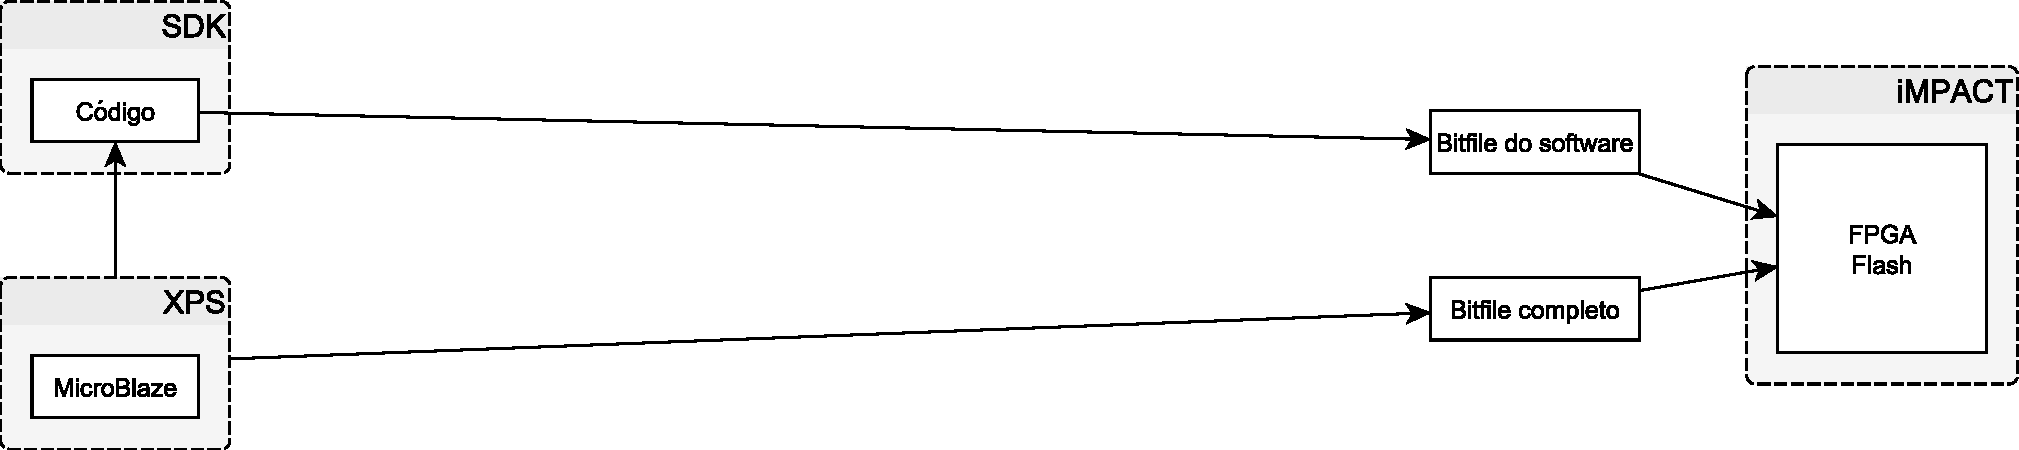
\includegraphics[height=100px]{fig/c3_desenvolvimento/ex2/softwareflow.pdf}
\caption{Foto ilustrativa do fluxo de ferramentas para o desenvolvimento de sistemas com MicroBlaze, extraído de \cite{ug081}.}
\label{fig:ex2:softwareflow}
\end{figure}

\subsubsection{MicroBlaze}
O MicroBlaze é um microprocessador otimizado para implementação em FPGAs da Xilinx \cite{ug081}.
Ele possui 32 registradores genéricos de 32 bits, instruções de 32 bits e endereços de 32 bits.
Seu \textit{pipeline} possui 3 ou 5 estágios e é construido em torno da arquitetura Harvard, como pode ser observado na figura \ref{fig:ex3:microblazecore}.
Todas as outras configurações, tais como o uso de \textit{Big Endian} ou \textit{Little Endian}, por exemplo, são opcionais \cite{ug081}.

\begin{figure}[h]
\centering
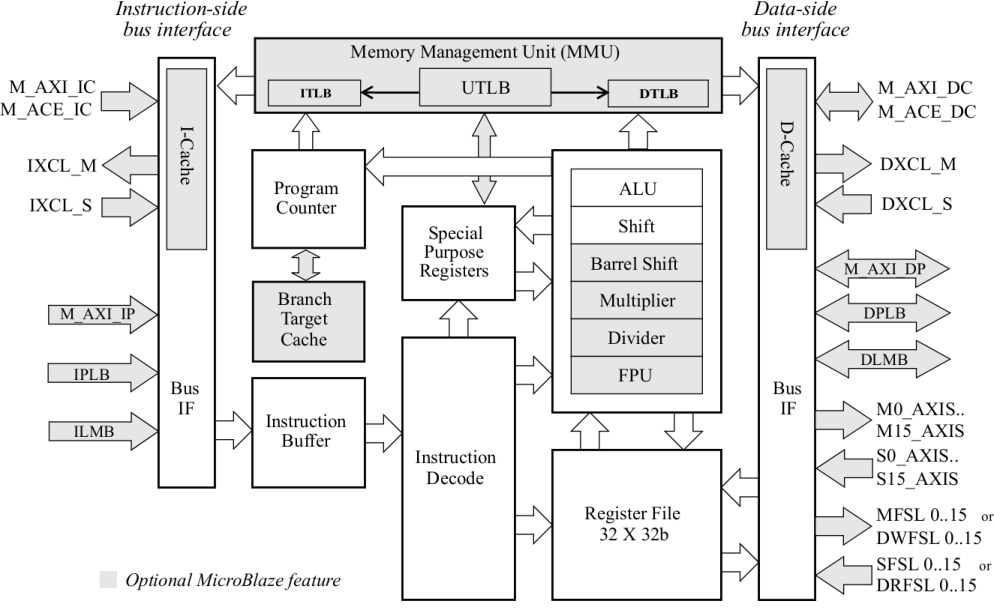
\includegraphics[width=0.75\textwidth]{fig/c3_desenvolvimento/ex2/MicroBlaze_Core.pdf}
\caption{Diagrama de blocos do MicroBlaze.}
\label{fig:ex3:microblazecore}
\end{figure}

O MicroBlaze permite o uso de diversas interfaces para comunicação com seus diversos periféricos, dentre elas a PLB, a LMB, a AXI e a ACE \cite{ug081}.
A interface mais atual suportada, e que foi utilizada neste experimento, é a Advanced eXtensible Interface 4 (AXI4) \cite{ug081, ug761}.
A AXI4 é uma interface mapeada em memória que oferece produtividade, flexibilidade e disponibilidade.
Ela possui três tipos de interfaces, a AXI4, a AXI4-Lite e a AXI4-Stream, onde as duas primeiras são compostam de 5 canais de comunicação: de leitura de endereço, de escrita de endereço, de leitura de dados, de escrita de dados e de escrita de resposta.

\subsubsection{XPS}
Para começar, deve-se abrir o programa e criar um novo projeto usando o \textit{Base System Builder} (BSB), opção que corresponde ao item superior esquerdo do menu da tela inicial.
Na janela que aparece, escolheu-se a placa de desenvolvimento Kintex-7 KC705 \textit{Evaluation Platform}, \textit{Board Revision} C, e a opção de um só processador no sistema, para simplificar o projeto.
Dando prosseguimento, escolheu-se os periféricos desejados segundo a figura \ref{fig:ex2:bsb_prerifericos} e o tamanho das memórias local, de intrução e de dados, quiça 64 KB.
Modificou-se ainda, como pode-se ver na figura \ref{fig:ex2:bsb_prerifericos}, o \textit{Baud Rate} da interface UART para 115200 bits/s e o C\_SPI\_MODE da QSPI\_FLASH para \qti{Quad SPI Mode}.

\begin{figure}[htp]
\centering
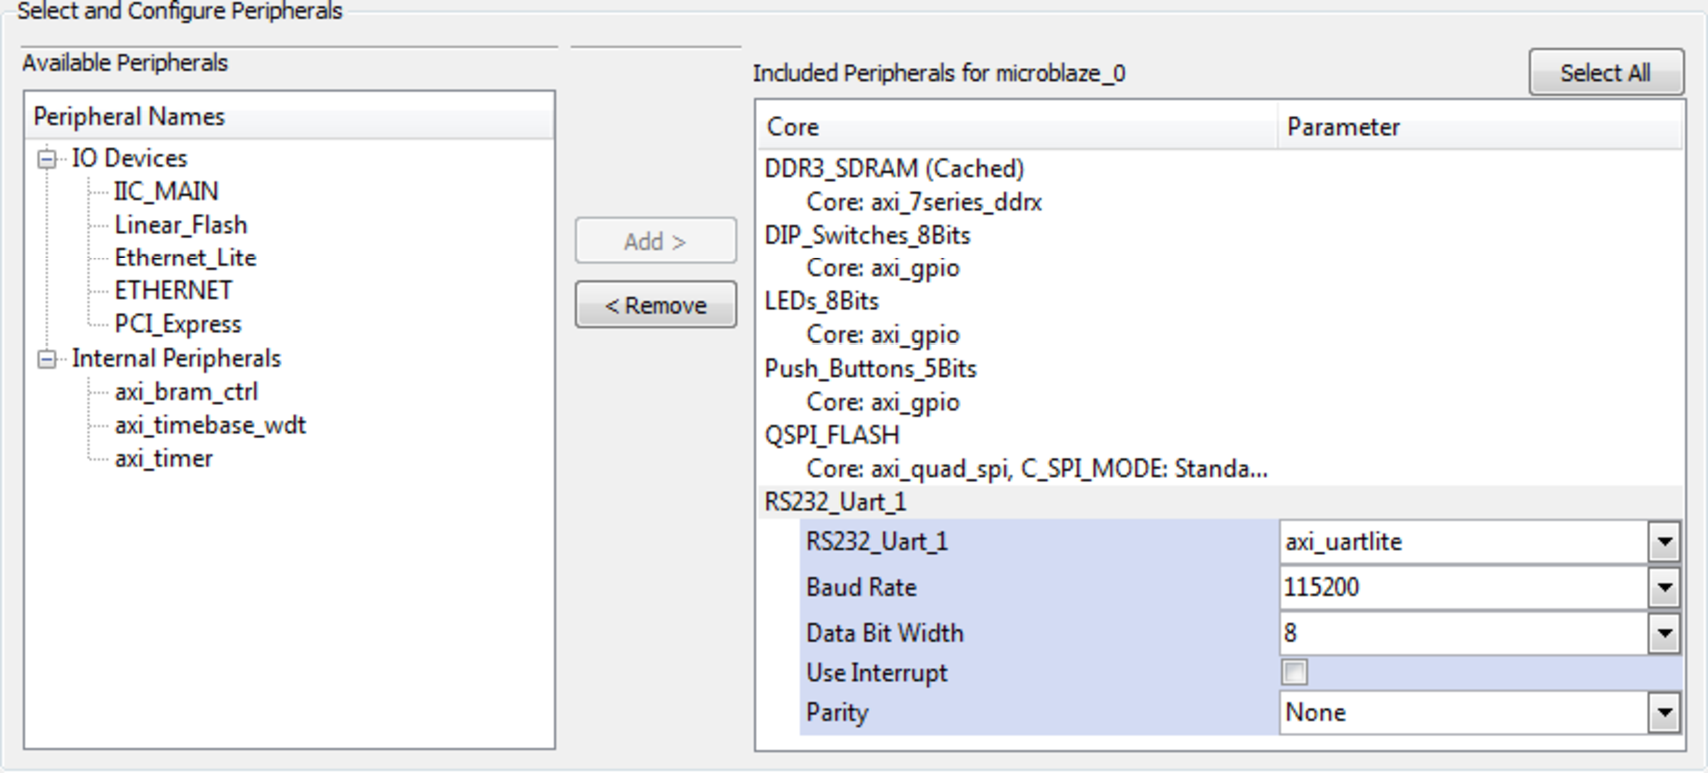
\includegraphics[width=0.9\textwidth]{fig/c3_desenvolvimento/ex2/BSB_AXI_flow.pdf}
\caption{Escolha dos periféricos no BSB do XPS.}
\label{fig:ex2:bsb_prerifericos}
\end{figure}

Antes de concluir o a construção do sistema, precisa-se ajustar os tamanhos das memórias e seus endereços, de forma que estes novos tamanhos possam ser corretamente acessados.
Isto pode ser feito na aba \textit{Addresses} do painel \textit{System Assembly View}.
Muda-se então o tamanho da memória SPI Flash para 128M, seu endereço base para 0x80000000, o tamanho da memória DDR3 para 1G e seu endereço base para 0xC0000000, conforme a figura \ref{fig:ex2:xps_enderecos}.
Note que o endereço-base da memória SPI Flash tem como única restrição de os 28 bits menos significativos iguais a zero e que o endereço-base da memória DDR3 tem esta mesma restrição para os 30 bits menos significativos.
Estas restrições são devido aos tamanhos das memórias e o alinhamento dos espaços de dados na memória.

\begin{figure}[htp]
\centering
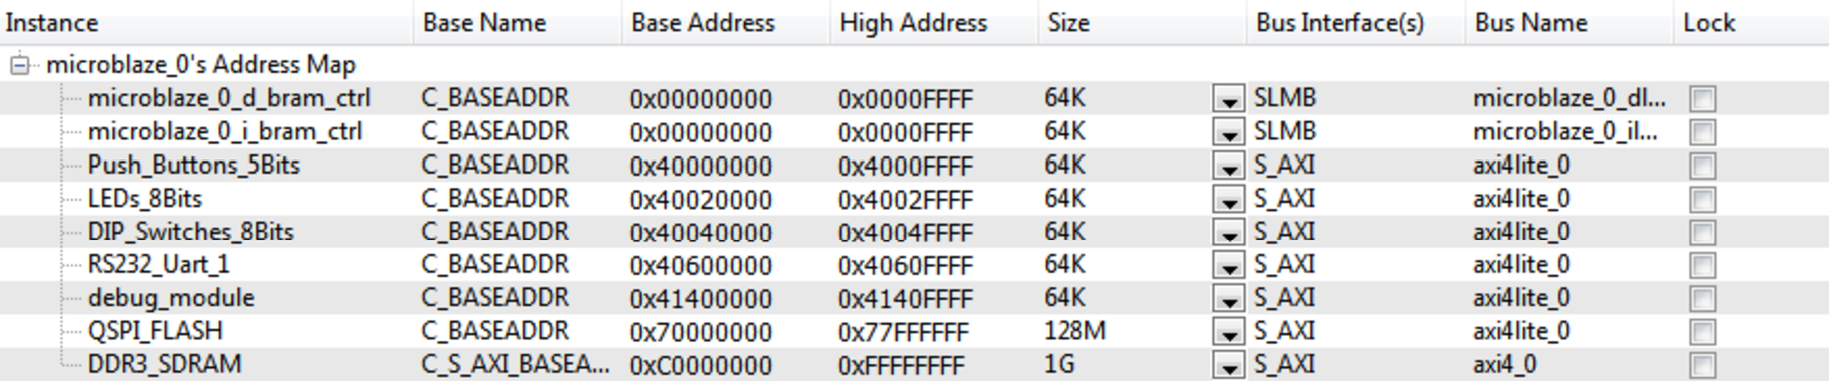
\includegraphics[width=0.8\textwidth]{fig/c3_desenvolvimento/ex2/xps_address.pdf}
\caption{Aba \textit{Addresses} do \textit{System Assembly View} indicando os ajustes dos endereços e tamanhos das memórias.}
\label{fig:ex2:xps_enderecos}
\end{figure}

Precisa-se agora modificar as posições de memória cobertas pela memória \textit{cache}.
Isto é feito clicando-se duas vezes sobre \qt{microblaze\_0} na aba \qt{\textit{Bus Interfaces}} do painel \qt{\textit{System Assembly View}}.
Na janela que se abre, clica-se  \qt{\textit{Next}} 3 vezes para chegar página sobre \textit{caches}.
Modifique os endereços nas duas colunas para 0xc0000000 e 0xffffffff, indicando que a memória de instruções e memória de dados podem acessar os endereços da memória DDR3.
Apenas os endereços contidos neste intervalo da memória de dados podem ser escritos.
Note que o sistema reserva para uso próprio os primeiros 64K endereços das memórias, que correspondem às posições com finais entre 0x0000 a 0x3fff.
A tentativa de uso destes endereços comprometerá o correto funcionamento do sistema.

Algumas outras configurações também podem ser ajustadas, mas não sao estritamente necessárias para este experimento.

O projeto pode ser sintetizado através do botão \qt{\textit{Generate Netlist}} localizado no menu a esquerda e no menu \qt{\textit{Hardware}} da barra de menus.
Este processo é demorado.
Quando terminado, pode-se exportar o projeto através do botão \qt{\textit{Export Design}} para abrir o SDK com as informações deste processador.
Na janela que aparecer, marque \qt{\textit{Include bitstream and BMM file}} e clique em \qt{\textit{Export \& Launch SDK}}.
Após a implementação do arquivo binário, a ferramenta SDK será aberta.

\subsubsection{SDK}
Quando a janela do SDK aparecer, ela perguntará onde se quer colocar o \textit{workspace}.
Uma boa opção é a pasta SDK criada dentro da pasta do projeto do sistema durante sua exportação, apesar desta escolha ser completamente arbitrária.
Escolhida a pasta, o ambiente de trabalho é aberto.

Começa-se o processo criando um projeto do tipo \qt{\textit{Board Support Package}}.
Este projeto compila automaticamente os drivers disponíveis para o projeto segundo as características do microcontrolador.
Em seguida, pode-se criar os projetos dos \textit{softwares} que irão embarcados.
Para isto, cria-se um projeto do tipo \qt{\textit{Application Project}}.
Na janela que se abre, nomeie o projeto e selecione a \qt{\textit{Board Support Package}} no \textit{dropdown} do item \qt{\textit{Board Support Package}}.
Na página seguinte, escolhe-se \qt{\textit{Empty Project}}.

Adiciona-se arquivos ao projeto tanto arrastando os códigos para ele quanto selecionando a opção \qt{\textit{New/Source File}} do menu que aparece quando se clica no projeto com o botão direito.
Note que o acesso a memória é feito simplesmente dereferenciando um ponteiro para a posição de memória desejada.
A escrita é feita do mesmo modo.
Encontra-se em anexo códigos-exemplo para o teste das memórias DDR3 e SPI Flash.

Antes de executar o programa, é interessante habilitar a opção de debugação.
Isto é feito através do menu \qt{\textit{Run}}, na opção \qt{\textit{Run Configurations...}}.
Na janela que aparece, na aba \qt{\textit{STDIO Connection}}, habilita-se a conexão do STDIO com o console e modifica-se o \qt{\textit{Baud Rate}} para 115200.
Clica-se então em \qt{\textit{Apply}} e em seguida \qt{\textit{Close}}.

A programação do FPGA pode ser feita através do menu \qt{\textit{Xilinx Tools}}, na opção \qt{\textit{Program FPGA}}.
Na janela que se abre, é padrão que as informações já estejam pré-preenchidas, mas caso isto não aconteça, procura-se pelos arquivos \qt{system.bit} e \qt{system\_bd.bmm} na pasta \qt{\textit{implementations}} na raíz do projeto do processador.
Clica-se em \qt{\textit{Program}} para inciar a programação.

Para se transferir o programa criado com o auxílio do SDK, seleciona-se o projeto deste programa, clica-se com o botão direito, seleciona-se o submenu \qt{\textit{Run As...}} e escolhe-se a opção \qt{\textit{1 Launch on Hardware (GDB)}}.
No caso dos códigos-exemplo, algumas informações são imprimidas no console caso tudo tenha ocorrido confome o esperado.

\subsection{Conclusão}
Conclui-se assim o experimento para o teste de programação das memórias.
Notou-se que existe muita pouca literatura no assunto, forçando o programador a fazer uso dos forúns de discussão e conhecimentos gerais de programação embarcada.
Apesar disso, o objetivo do experimento, quiça conseguir ler/escrever de/em endereços das memória DDR3 e SPI Flash específicos, foi atingido com sucesso.

\section{Experimento 3 - Teste do \textit{Bootloader}}
O \textit{bootloader}, como mencionado acima, é um sistema que carrega as informações de uma memória lenta, a SPI Flash foi escolhida, para uma memória rápida, a memória DDR3.
Usou-se um microcontrolador MicroBlaze com interfaces para as memórias SPI Flash e DDR3.
O experimento 2 foi dedicado a aprender a utilizar estas memórias.
Neste experimento, espera-se entender como é formado o arquivo binário para assim carregá-lo e interpretá-lo enquanto o transferindo para a memória DDR3.

Utilizará-se também o GPIO, que dá acesso aos pinos da placa, visto que é interessante que este subsistema possa sinalizar para os demais que o carregamento foi completado e informar algumas informações dos elementos transferidos, tais como tamanhos e posições iniciais.

\begin{figure}[htp]
\centering
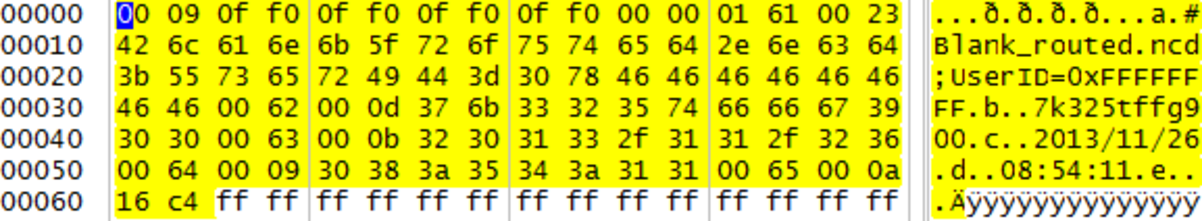
\includegraphics[width=0.8\textwidth]{fig/c3_desenvolvimento/ex3/hex_blank.pdf}
\caption{Cabeçalho do arquivo binário gerado no primeiro experimento para a configuração vazia.}
\label{fig:ex3:hex_blank}
\end{figure}

\subsection{Arquivo Binário}
O arquivo binário é formado por três partes: um cabeçalho, uma palavra para sincronia e a configuração propriamente dita \cite{ug470, xapp583}.
O cabeçalho é formado por chaves e tamanhos, indicando diversos campos deste.
Na tabela \ref{tab:ex3:hex_blank} pode-se observar os tamanhos e campos apresentados na figura \ref{fig:ex3:hex_blank}.
A figura \ref{fig:ex3:hex_blank} possui os primeiros 112 bytes, dos quais os primeiros 98 estão selecionados, da configuração parcial vazia construida no experimento 1.
O primeiro conjunto tamanho/chave indica, através da sequência de de palavras 0x0f, que a configuração é válida.
Se estas palavras fossem 0x00 indicariam que a configuração não é mais válida, e se contivessem 0xff indicariam que a configuração está vazia.

O cabeçalho descrito na tabela \ref{tab:ex3:hex_blank} contém pelo menos duas informações muito interessantes: o identificador do dispositivo alvo, que permite verificar a compatibilidade entre a configuração e o dispositivo que a está recebendo, e o tamanho da configuração, que permite que ela seja carregada de forma dinâmica sem necessidade de mais informações.

\begin{table}[htp]
\centering
\begin{tabular}{cp{4cm}p{7.5cm}}
Tamanho & Chave & Significado\\ \hline
2 bytes & 9 (0x00 09) & Tamanho em bytes do próximo campo \\ \hline
9 bytes & 0x0f f0 0f f0 0f f0 0f f0 00 & Indica que a configuração a seguir é válida. \\ \hline
2 bytes & 1 (0x00 01) & Tamanho em bytes do próximo campo\\ \hline
1 byte & "a" (0x61) & Indica que os próximos campos conterão informações sobre o projeto e sobre a configuração. \\ \hline
2 bytes & 35 (0x00 23) & Tamanho em bytes do próximo campo \\ \hline
35 bytes & Blank\_routed.ncd;\qquad UserID=0xFFFFFFFF & Apresenta o nome do \textit{netlist} e o identificador do usuário. 0x00 ao final indica o final da string. \\ \hline
1 byte & "b" (0x62) & Indica que o próximo campo é um indentificador do dispositivo-alvo. \\ \hline
2 bytes & 13 (0x00 0d) & Tamanho em bytes do próximo campo \\ \hline
13 bytes & 7k325tffg900 & Identificador do dispositivo-alvo. 0x00 ao final indica o final da string. \\ \hline
1 byte & "c" (0x63) & Indica que o próximo campo é a data de sintese da configuração. \\ \hline
2 bytes & 11 bytes (0x00 0b) & Tamanho em bytes do próximo campo \\ \hline
11 bytes & 2013/11/26 & Data da síntese da configuração. \\ \hline
1 byte & "d" (0x64) & Indica que o próximo campo é a hora de síntese da configuração. \\ \hline
2 bytes & 9 bytes (0x00 09) & Tamanho em bytes do próximo campo \\ \hline
9 bytes & 08:54:11 & Hora de síntese da configuração. \\ \hline
1 byte & "e" (0x65) & Indica que os próximos 8 bytes contém o tamanho da configuração. \\ \hline
4 bytes & 661188 (0x00 0a 16 c4) & Tamanho em bytes da configuração a partir desta posição. \\\hline
\end{tabular}
\caption{Descrição do cabeçalho dos arquivos binários.}
\label{tab:ex3:hex_blank}
\end{table}

Ainda no cabeçalho, tem-se um 32 bytes de espaçamento preenchidos por com \qt{0xff}.
Em seguida, tem-se os bytes para autodetecção de largura de banda \cite{ug470, xapp583}.
Estes bytes (\qt{0x00 00 00 bb 11 22 00 44}) são usados no modo de configuração paralelo para detectar automaticamente a largura de banda do arquivo de configuração.
O modo serial ignora todos os bits anteriores a palavra de sincronia \cite{xapp583}.
Estes bits são então usados apenas para pré-processamento do arquivo binário.

A palavra de sincronia (\qt{0xaa 99 ff 66}), encontrada a seguida, serve para indicar o inicio da configuração proprimamente dita e para alinhar o fluxo de dados nos registradores internos.

\paragraph{Inversão dos bytes} A interface ICAP e a ICAPE2, similares a interface SelectMAP \cite{wp374}, precisa de uma inversão na ordem dos bits nos bytes da configuração, incluindo a palavra de sincronia \cite{xapp502}.
Esta inversão é necessária apenas no uso destas três interfaces.
Note que alguns tipos de arquivos sintetisados, como o MCS e o HEX, já podem ter estes bytes invertidos não sendo necessário invertê-los novamente \cite{ug470}.

\subsection{Inicialização da Memória SPI Flash}
A memória SPI Flash, assim como todas as outras, precisa de um procedimento especial para poder ser inicializada com informações arbitrárias \cite{xapp694}.
Em geral, as únicas informações que podem ser gravadas nas memórias não-voláteis são configurações para o FPGA e programas para algum MicroBlaze embarcado \cite{ug111}.
Este processo é conhecido como programação indireta da memória Flash \cite{xapp586}.

\subsubsection{Compilação} Para a realização da programação indireta, o arquivo binário precisa ser compilado de forma a gerar um padrão de bits compatível.
Este procedimento é realizado na etapa de construção do processador.
Quando não especificado, o arquivo binário gerado utiliza a interface QSPI x1, que possui banda de transferência de 1 bit por leitura/escrita,  e relógio de frequência 3 MHz.
Com estas configurações, a programação do sistema demora apenas 1 minutos e 30 segundos \cite{xapp586}, mas pode ser ainda mais reduzido.

No PlanAhead, as configurações de compilação podem ser modificadas através do arquivo \qt{bitgen.ut} localizado na pasta \qt{etc} do projeto.
Através da opção \qt{-g SPI\_buswidth:X}, onde X pode ser 1, 2 ou 4, pode-se alterar a interface utilizada neste tipo de programação \cite{ug628, xapp576}, sendo a x4 a mais eficiente.
Pode-se ainda forçar a opção \qt{-g ConfigRate\_en:Y}, onde Y pode ser 3, 6, 9, 12, 16, 22, 26, 33, 40, 50 ou 66, para se utilizar de relógios de variadas frequências e obter assim o modo de configuração mais adequado para a memória em questão \cite{xapp586, ug628, ug810}.
Existe também a opção \qt{-g SPI\_Fall\_Edge:Yes}, que permite melhora margens de tempo e pode aumentar as taxas de leitura para configurações \cite{ug628, ug586}.
Uma opção alternativa é utilizar um relógio externo através da opção \qt{-g ExtMasterCclk\_en:Z}, onde Z pode ser \qt{Disable}, \qt{div-8}, \qt{div-4}, \qt{div-2} e \qt{div-1}.

\subsubsection{Arquivo de Memória PROM}
Após compilado o projeto, seu arquivo binário e qualquer outra informação a ser programada na memória Flash precisa ser adicionada a um arquivo do tipo MCS.
Este processo é necessário para que o iMPACT consiga carregar e programar a memória Flash de forma correta.

Pode-se construir este arquivo de memória PROM através do iMPACT.
No momento da criação do novo projeto do iMPACT, seleciona-se a opção \qt{\textit{Prepare a PROM File}}.
Na janela seguinte, seleciona-se \qti{SPI Flash/Configure Single FPGA} no primeiro painel e \qt{128M} no segundo e modifica-se \qti{Add Non-Configuration Data Files} para \qt{Yes}, conforme mostrado na figura \ref{fig:ex3:prom_file}.

\begin{figure}[htp]
\centering
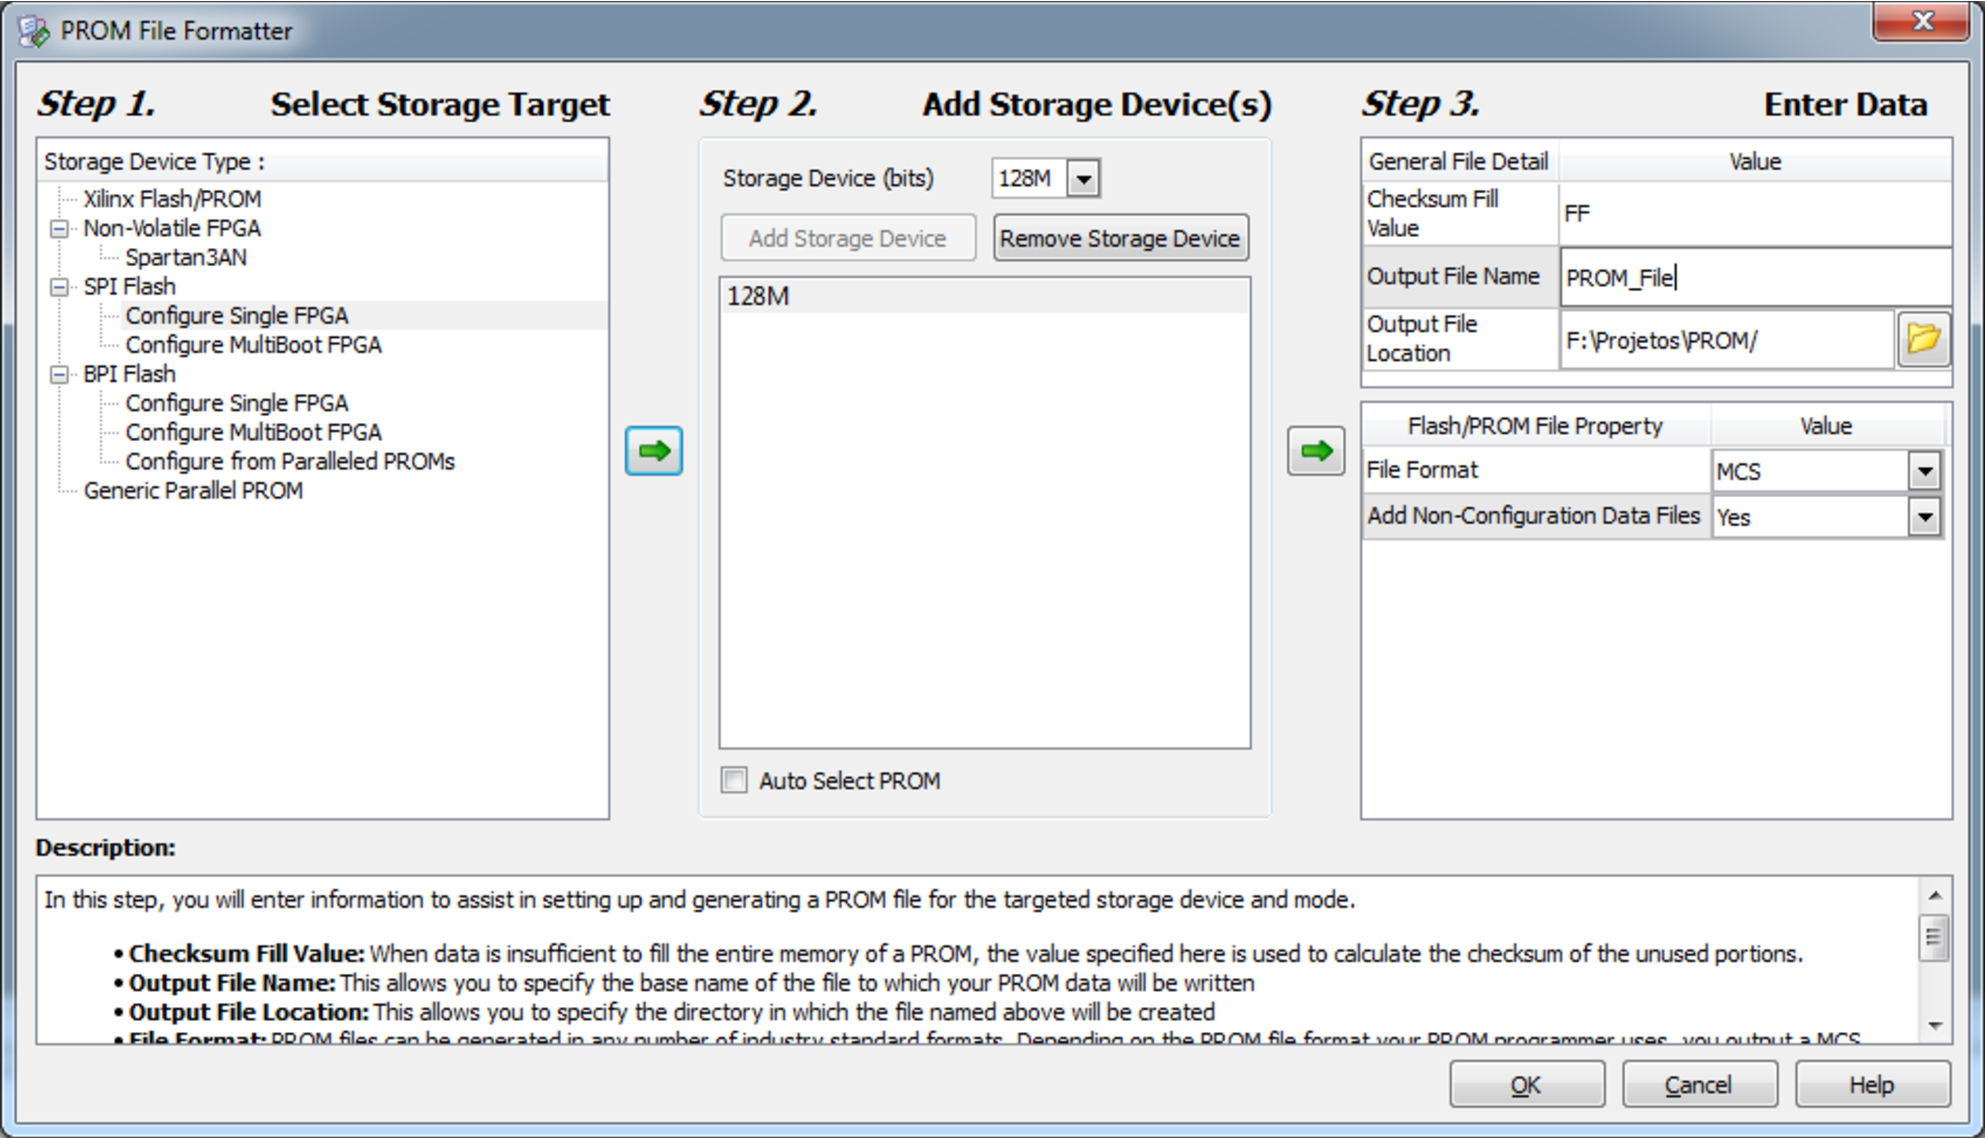
\includegraphics[width=0.9\textwidth]{fig/c3_desenvolvimento/ex3/PROM_File.pdf}
\caption{Janela para criação de um arquivo de memória PROM com as configurações devidamente ajustadas.}
\label{fig:ex3:prom_file}
\end{figure}

Em seguida, adicionam-se os arquivos binários que se deseja programar na memória Flash.
O primeiro arquivo a se adicionar é o de configuração total.
Este arquivo é carregado durante o procedimento de inicio do FPGA.
Apenas um arquivo deste tipo precisa ser carregado neste experimento, apesar de ser possível realizar um projeto com diversas revisões de configurações ou múltiplas possibilidades de configurações de \textit{boot} \cite{xapp468, xapp1100}.
Para rejeitar a adicão de outras configurações, deve-se clicar em \qti{No} na mensagem de título \qti{Add Device}.

\begin{figure}[htp]
\centering
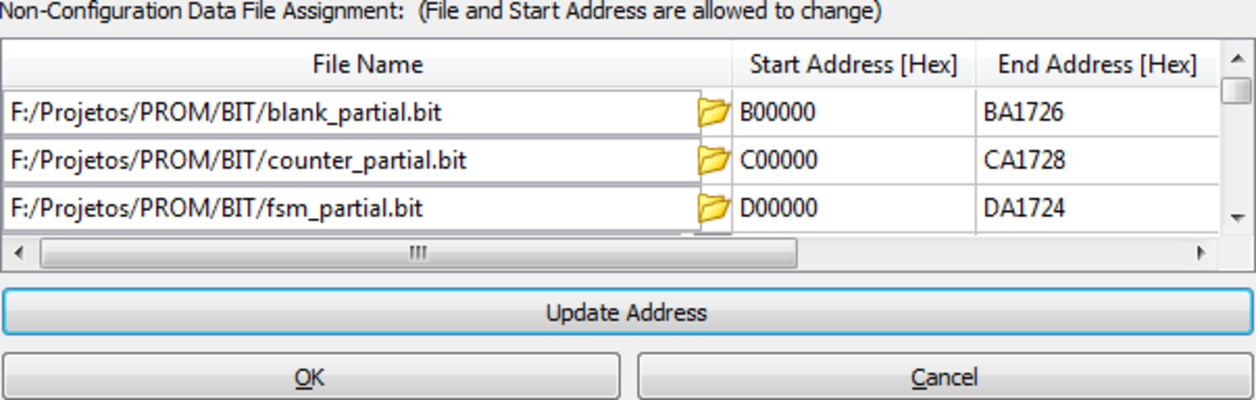
\includegraphics[width=0.75\textwidth]{fig/c3_desenvolvimento/ex3/PROM_Addr.pdf}
\caption{Janela para criação de um arquivo de memória PROM com as configurações devidamente ajustadas.}
\label{fig:ex3:prom_addr}
\end{figure}

A mensagem seguinte, \qti{Add Data File}, faz referência a adição de arquivos de dados neste projeto.
Clicando-se em \qti{Yes}, uma janela aparece com informações de endereçamento.
Pode-se aceitar os valores iniciais.
Estes arquivos podem ter qualquer conteúdo, mas o programa espera arquivos gerados pelo SDK, sendo necessário mudar a configuração de arquivos apresentados para \qti{All Files (*.*)}.
Após adicionar-se todos os arquivos, deve-se clicar em \qti{No} na janela de inclusão de novos arquivos de dados.
Ao se fazer isto, uma janela para indicação dos endereços é mostrada.
Recomenda-se mudar os endereços de início (\qti{Start Address}) para valores arredondados, como 0xB00000, 0xC00000 e 0xD00000, obedecendo os endereços das revisões, de forma a facilitar o trabalho de programação do sistema embarcado.
O botão \qti{Update Address} deve ser clicado para ajustar os endereços de fim (\qti{End Address}) antes de se prosseguir, obtendo-se algo similar a figura \ref{fig:ex3:prom_addr}.

O último passo é gerar o arquivo, o que pode ser feito através do menu \qti{Operations} ou do painel \qti{iMPACT Processes}, selecionando-se a opção \qti{Generate File...}.
Este processo é rapido e resulta em um arquivo MCS gerado na pasta destino definida no passo da figura \ref{fig:ex3:prom_file}.

\subsection{Teste}
O teste deste experimento compreende a construção de um sistema microprocessado que carregue os arquivos binários da memória SPI Flash para a memória DDR3.
Este experimento contribuirá para a compreenção do processo de inicialização de memórias não-voláteis e do tratamento do cabeçalho dos arquivos binários.
Usará-se os programas XPS, SDK, que fazem parte do Embedded Development Kit (EDK), data2mem e iMPACT.

\subsubsection{XPS}
Utilizou-se o mesmo microcontrolador MicroBlaze construido no experimento passado, não sendo necessária nenhuma modificação.
A interface SPI utilizada aqui foi a padrão, x1, por motivos de simplificação do projeto.
O uso de uma interface x4 diminuiria o tempo de programação em 4 vezes, o que não é fator crítico para este experimento, mas acarretaria na necessidade de recompilar todos os projetos desenvolvidos até agora.

\subsubsection{SDK}
Logo após a construção do microcontrolador, recomenda-se construir o projeto do programa embarcado.
O procedimento para o SDK nesse caso é bem semelhante ao dos experimentos anteriores.
Apenas as diferenças serão citadas a seguir.

Desta vez, tem-se como objetivo fazer com que o sistema se carregue e entre em funcionamento de forma autônoma.
Para isto, precisa-se, depois da inclusão dos devidos arquivos, presentes no anexo, gerar o \textit{linker script}.
Este arquivo descreve como o arquivo binário do \textit{bootloader} deve ser armazenado na memória interna do FPGA para execução.
Este \textit{script} pode ser gerado clicando-se com o botão direito sobre o projeto do prgrama embarcado e selecionando-se a opção \qti{Generate Linker Script...} ou selecionando-se o projeto, abrindo-se o menu \qti{Xilinx Tools} e selecionando-se a opção do mesmo nome.
Para o escopo deste experimento, as configurações apresentadas na janela que se abre são suficientes, bastando clicar em \qti{Generate}.
A criação deste \textit{script} permite agora que se utilize o programa \qt{data2mem} para construir um arquivo binário de configuração com um programa embarcado pré-programado.

\subsubsection{data2mem}


\subsubsection{Arquivo de Memória PROM}
Para a construção de um arquivo de memória PROM como descrito anteriormente, faz-se necessário que todos os elementos sejam compilados para uma mesma interface SPI.
O uso de interfaces diferentes pode gerar erros na programação da memória Flash.

\subsection{Conclusão}


\todo{Explicar como fui para o próximo experimento}
\section{Experimento 4 - Teste da Autoreconfiguração com \textit{Bootloader} Dedicado}
\todo{Descrever o experimento 4}

\subsubsection{Registrador de \textit{Status}}
Este registrador, acessado através de uma sequência predefinida de comandos pela interface ICAPE2 \cite{ug470 - pp108}, informa 

\todo{Explicar como fui para o próximo experimento}
\section{Experimento 5 - Teste da Autoreconfiguração}
\todo{Descrever o experimento 5}
\todo{Explicar como fui para o próximo experimento}

\ifx\compilewholereport\undefined
	\bibliographystyle{plain} 
	%\bibliography{bibliografia.bib}
	\newsavebox\mytempbib\savebox\mytempbib{\parbox{\textwidth}{\bibliography{bibliografia}}}

	\end{document}
\fi 

\part{Resultados e Conclusões}
% *** Resultados Experimentais ***
%TCIDATA{LaTeXparent=0,0,relatorio.tex}
\ifx\compilewholereport\undefined  
	\documentclass[11pt,a4paper,oneside]{book}
	
	% Escolher um dos seguintes formatos:
	\usepackage{ft2unb} % segue padrão de fontes do Latex
	
	% Pacotes
	\usepackage{graphicx}
	\usepackage{amsfonts}
	\usepackage{amsmath}
	\usepackage{amssymb}
	\usepackage[thmmarks,amsmath]{ntheorem}
	\usepackage{boxedminipage}
	\usepackage{theorem}
	\usepackage{fancybox}
	\usepackage{fancyhdr}
	\usepackage{url}
	\usepackage{afterpage}
	\usepackage{xcolor}
	\usepackage{rotating}
	\usepackage{makeidx}
	\usepackage{indentfirst}
	\usepackage{subcaption}
	\usepackage{todonotes}
	\usepackage{listings}
	\presetkeys{todonotes}{inline}{} 
	
	\begin{document}
	\frontmatter
	\tableofcontents
	\mainmatter 
	
	%%%%%%%%%%%%%%%%%%%%%%%%%%%%
	%%%%%%%% Apagar coisas acima
	%%%%%%%%%%%%%%%%%%%%%%%%%%%%
	\newcommand\qt[1]{\lq\lq{}#1\rq\rq{}}
	\newcommand\qti[1]{\lq\lq{}\textit{#1}\rq\rq{}}
\fi
                      
\chapter{Resultados}\label{CapExperimentos}

% Resumo opcional. Comentar se não usar.
\resumodocapitulo{Este capítulo tem como objetivo apresentar um resumo dos resultados alcançados pelos vários experimentos realizados, uma vez que os resultados específicos estão contidos nos capítulos dos respectivos experimentos.}
\vspace{0.8cm}

Os experimentos realizados neste trabalhos serviram para construir um conhecimento profundo em torno do desenvolvimento de aplicações reconfiguráveis baseadas em FPGAs.
Entende-se que as partes mais importantes deste conhecimento, além da capacidade de resolução de problemas relacionados, é o entendimento do fluxo de desenvolvimento necessário.
Este fluxo, resumido na figura \ref{fig:res:prfileflow}, não é descrito claramente na literatura, tornando esta tecnologia complicada de se estudar e utilizar.
O que buscou-se fazer com os experimentos foi determinar uma linha de pensamento sólida e lógica, que ajudasse a determinar este fluxo mais facilmente.

\begin{figure}[htp]
\centering
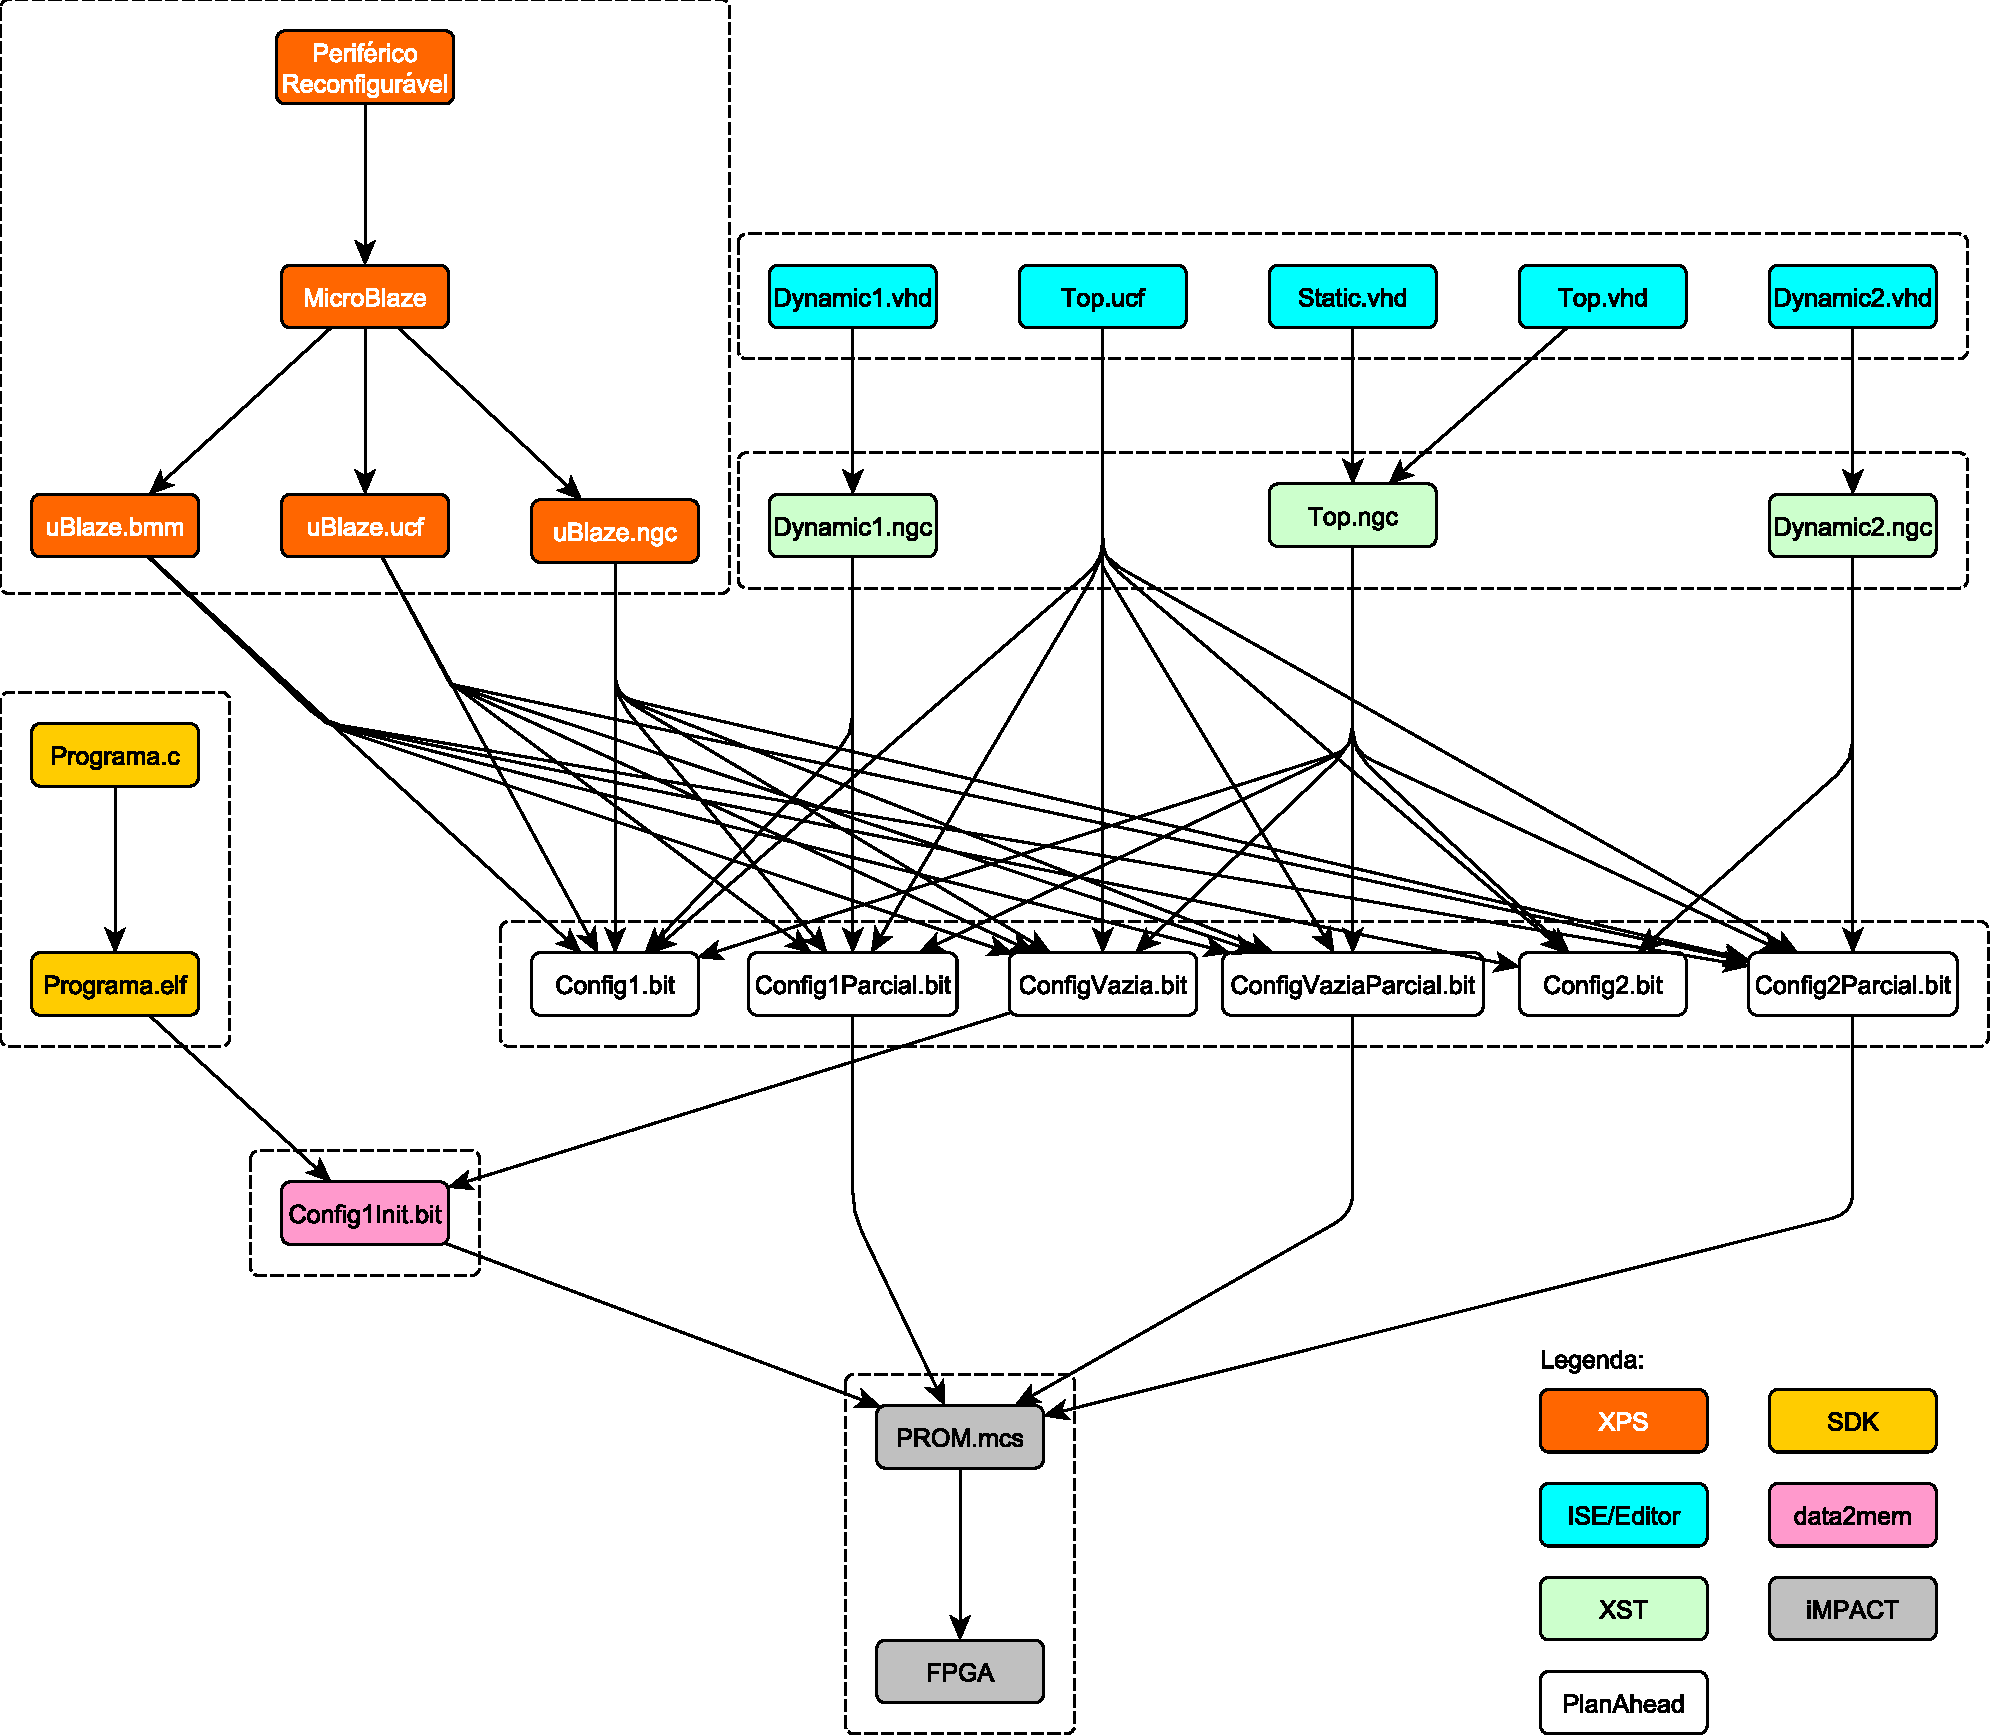
\includegraphics[width=\textwidth]{fig/resultados/prfileflow.pdf}
\caption{Fluxo de projeto para aplicações reconfiguráveis usando as ferramentas da Xilinx. Cada bloco representa um arquivo gerado com o auxílio de alguma ferramentas. As arestas indicam que tal arquivo foi utilizado para gerar o seguinte. Arquivos gerados pelas mesmas ferramentas estão agrupados com uma linha contínuo, no caso de um arquivo de construção obrigatória, ou com uma linha tracejada, no caso de arquivos cuja construção depende dos requisitos do projeto. Estão indicados ainda os tempos, incluindo os tempos das interações necessárias com o usuário, estimados para a construção de cada arquivo. Note que este fluxo é apenas o indicado para a maioria dos projetos, mas que existem projetos que seguem fluxos diferentes, seja por opção ou necessidade.}
\label{fig:res:prfileflow}
\end{figure}

Devido ao caráter de estudo de um tecnologia, não se faz necessária a inclusão de relatórios de utilização ou desempenho.
Estes elementos podem ser estudados mais a fundo de forma separada.
Sua inclusão neste trabalho poderia acarretar na perda do foco principal, quiça autorreconfiguração.

É interessante notar que um dos experimentos, especificamente o quarto, teve de ser reavaliado, tendo sido considerado mal sucedido.
O motivo para tal foi o encontro de diversos problemas graves que desaceleraram o desenvolvimento, comprometendo a realização deste trabalho.
Estes problemas foram causados em parte pela má integração entre as diversas ferramentas da Xilinx, mas em maior parte por problemas relacionados a memória DDR3 e seus requisitos de temporização.
Apesar disso, conseguiu-se perceber este impasse a tempo e reformular este experimento de tal forma que ele fosse alcançavel.

Através da realização dos experimentos de 1 a 4, juntou-se o conhecimento necessário que culminou na realização do experimento 5.
Este por sua vez, serviu para clarificar alguns detalhes referentes a integração de projetos do XPS e do PlanAhead, abrindo um leque de possibilidades de continuação deste trabalho.

\section{Análise de Tempo}
O fator mais explicitamente influenciador dos resultados deste projeto foi o tempo, especialmente quando aliado ao caráter experimental deste projeto.
Pode-se observar da figura \ref{fig:res:prfileflow} que cada ferramenta possui um tempo máximo e mínimo necessários para seu uso.
Estes tempos foram estimados com base nos tempos gastos nos experimentos, considerando-se que nenhum erro grave tenha acontecido.

A figura \ref{fig:res:prtimeflow} possui uma representação alternativa, que mostra a construção do projeto como um \textit{pipeline}.
As informações acima deste grafo direcionado representam os tempos, máximo e mínimo, gastos em cada etapa e as informações abaixo mostram o tempo gasto acumulado, máximo e mínimo, desde o início do projeto.
Note que, mesmo desconsiderando-se os tempos de desenvolvimento de periféricos, programas embarcados e comportamento do \textit{hardware}, leva-se no mínimo 1 hora e 47 minutos.
Considerando-se ainda que a maior parte dos erros é apresentada na etapa final da ferramenta PlanAhead, pode-se observar que gastou-se pelo menos 1 hora e 30 minutos por tentativa de implementação.

\begin{figure}[htp]
\centering
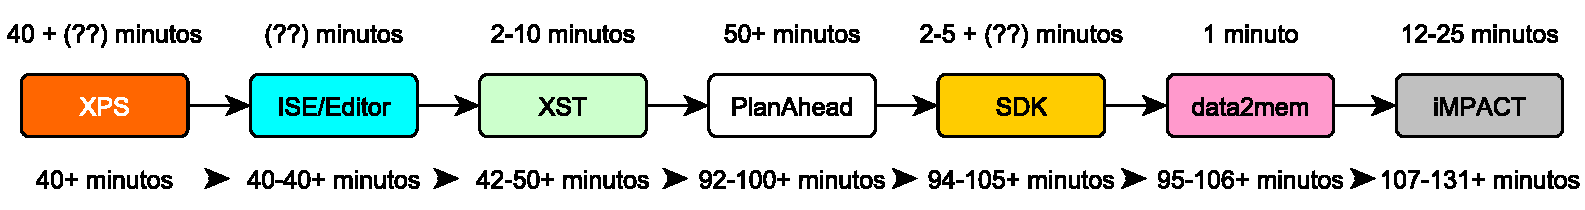
\includegraphics[width=\textwidth]{fig/resultados/prtimeflow.pdf}
\caption{Representação do fluxo de projeto através de um \textit{pipeline}. As informações acima dele indicam o tempo mínimo e máximo gasto em cada etapa, sendo que as etapas que possuem alguma fase de desenvolvimento apresentam um \lq\lq{}(??)\rq\rq{} para indicar que não tem como estimar o tempo gasto. As informações abaixo indicam o tempo mínimo e máximo gasto acumulado desde o início do projeto. A presença do sinal \lq\lq{}+\rq\rq{} indica que o valor apresentado é apenas uma estimativa empírica do valor máximo, podendo este ser ainda maior.}
\label{fig:res:prtimeflow}
\end{figure}

\ifx\compilewholereport\undefined
	\bibliographystyle{plain}
	\newsavebox\mytempbib\savebox\mytempbib{\parbox{\textwidth}{\bibliography{bibliografia}}}

	\listoftodos
	\end{document}
\fi

% *** Conclusões
%TCIDATA{LaTeXparent=0,0,relatorio.tex}
                      

\chapter{Conclus\~{o}es}\label{CapConclusoes}
No decorrer do desenvolvimento deste trabalho, pode-se observar a forma correta de se realizar projetos para autorrenconfiguração.
Por causa disso, considera-se que o trabalho foi bem sucedido.

O experimento 1 mostra e explica como realizar a reconfiguração dinâmica através de um computador.
Este experimento foi importante para comprovar o conceito e a capacidade do kit de suportar esta tecnologia.
O experimento 2 aborda o desenvolvimento de um microcontrolador MicroBlaze com periféricos para o controle de memórias QSPI Flash e DDR3.
Como foi explicado, memórias apresentam um papel extremamente importante na autorreconfiguração uma vez que nela a placa deve usar apenas recursos próprios para tudo.
O experimento 3 apresenta um estudo sobre o arquivo binário carregado pelas interfaces de reconfiguração, bem como o desenvolvimento de um programa capaz de interpretá-lo.
Este experimento permitiu ainda um maior entendimento sobre a inicialização da memória Flash para que ela fosse acessada em execuções subsequêntes.
O experimento 4, o único que fracassou, foi uma tentiva de se construir um sistema que carregasse as configurações da memória Flash para a memória DDR3 para então transmití-la as interfaces de reconfiguração.
Diversos problemas surgiram com relação a memória DDR3, forçando a removê-la do sistema, e algumas dúvidas surgiram com relação a inicialização arquivo binário final com o programa embarcado.
No experimento 5, conseguiu-se solucionar o problema da inicialização do arquivo binário, obtendo-se ao final um sistema autenticamente autorreconfigurável.
O módulo reconfigurável, porém, fazia parte do microcontrolador, interagindo com ele através da interface AXI Lite.

Sabe-se que existem formas mais eficientes e interessantes de se implementar a autorreconfiguração.
Um exemplo é a repetição do experimento 5 onde o módulo reconfigurável não esteja atrelado ao microcontrolador, mas apenas a um componente de interfaceamento \lq\lq{}Top\rq\rq{}.
Outra possibilidade é a implementação do microcontrolador com controladores para a memória DDR3 dentro de uma partição reconfigurável.
Sendo assim, durante o início do sistema, o microcontrolador poderia carregar e interpretar as configurações da memória Flash para a memória DDR3 e sinalizar o término para um controlador externo, que então reconfiguraria o microcontrolador para um controlador de memória DDR3, permitindo que as configurações fossem lidas pelo \textit{hardware}.
Observa-se que ainda é possível construir um sistema totalmente independente de microcontroladores, apesar de isto aumentar muito a complexidade do projeto.

%%%%%%%%%%%%%%%%%%%%%%%%%%%%%%%%%%%%%%%%%%%%%%%%%%%%%%%%%%%%%%%%%%%%%%%%%
% Referências bibliográficas
%%%%%%%%%%%%%%%%%%%%%%%%%%%%%%%%%%%%%%%%%%%%%%%%%%%%%%%%%%%%%%%%%%%%%%%%%
%\bibliographystyle{abnt-num} % use este estilo para ABNT numérico
%\bibliographystyle{abnt-alf} % use este estilo para ABNT alfa-numérico
\renewcommand{\bibname}{REFERÊNCIAS BIBLIOGRÁFICAS}
\addcontentsline{toc}{chapter}{REFERÊNCIAS BIBLIOGRÁFICAS}
\bibliography{bibliografia}
%
%%%%%%%%%%%%%%%%%%%%%%%%%%%%%%%%%%%%%%%%%%%%%%%%%%%%%%%%%%%%%%%%%%%%%%%%%%
%% Anexos
%%%%%%%%%%%%%%%%%%%%%%%%%%%%%%%%%%%%%%%%%%%%%%%%%%%%%%%%%%%%%%%%%%%%%%%%%%
%\anexos
%\makeatletter % não retirar estes comandos
%\renewcommand{\@makechapterhead}[1]{%
%  {\parindent \z@ \raggedleft \setfontarial\bfseries 
%        \LARGE \thechapter. \space\space  
%    \uppercase{#1}\par
%    \vskip 40\p@
%  }
%}
%\makeatother

%% *** Anexo I: Diagramas esquemáticos ***
%%TCIDATA{LaTeXparent=0,0,relatorio.tex}

\chapter{Diagramas Esquemáticos}\label{AnEsquematicos}


%\refstepcounter{noAnexo}
%
%% *** Anexo II: Descrição do CD ***
%%TCIDATA{LaTeXparent=0,0,relatorio.tex}

\chapter{Descrição do conteúdo do CD}\label{AnCD}

%\refstepcounter{noAnexo}

% Acrescente mais anexos conforme julgar necessário.
\end{document}

